% b6c_sizing_theory.tex
% Theory companion of the B6C sizing formula sheet (b6c_sizing_formulas.tex, Rev. 01): derivation of the sizing relations,
% overlap and its compensation, reverse recovery and Qrr, RC snubber criteria, fuses, LC filter, iteration loops.
% pwr-control template (AAA_template_latex_settings). Figure data: b6c_theory_figs.py; numbers of the example: b6c_example_calc.py.
% Compile: pdflatex b6c_sizing_theory.tex  (twice, for references)
% Rev. 00 - 2026-10-03 - first issue
\documentclass[10pt,a4paper]{scrartcl}
% ===================== PACKAGES =====================
\usepackage[british]{babel}
\usepackage[tmargin=1in, bmargin=1in, lmargin=0.75in, rmargin=0.75in]{geometry}
\usepackage[dvipsnames,table]{xcolor}  % prima di tikz, listings, ecc.

\usepackage{tikz}
\usepackage{graphicx}
\usepackage{pgfplots}
\pgfplotsset{width=12cm, compat=1.9}
\usepackage{setspace}
\usepackage{chemmacros}
\usepackage{chemfig}
\usepackage{esint}
\usepackage{tabularray}
\usepackage{makeidx}
\usepackage{epstopdf}
\usepackage{amssymb}
\usepackage{mathrsfs}
\usepackage{bm}
\usepackage{amsmath}
\usepackage{enumitem}
\usepackage[english]{varioref}
\usepackage{lipsum}
\usepackage{fancyhdr}
\usepackage{float}
\usepackage{empheq}
\usepackage[framemethod=tikz]{mdframed}
\numberwithin{equation}{section}
\usepackage{eso-pic}
\usepackage{calc}
\usepackage{nccmath}
\usepackage{caption}
\usepackage{subcaption}
\usepackage{gensymb}
\usepackage{amsfonts, amsthm, epsfig, epstopdf, titling, url, array}
\usepackage{tabularx}
\usepackage{makecell}
\usepackage{booktabs}
\usepackage{array}
\usepackage{siunitx}
\sisetup{input-digits=0123456789\pi}
\usepackage[symbol]{footmisc}
\usepackage{multicol}
\usepackage{boondox-cal}
\usepackage{blindtext}
\usepackage{changepage}
\usepackage{nomencl}
\usepackage{hyperref}
\usepackage{xurl}
\usepackage{ragged2e}
\usepackage[version=4]{mhchem}  % ← conflitto di opzioni
\usepackage{longtable}
\usepackage{chemformula}
\usetikzlibrary{arrows.meta,positioning,calc}

% ===================== SI UNITS =====================
\DeclareSIUnit\atm{atm}
\DeclareSIUnit{\var}{var}
\DeclareSIUnit{\pu}{p.u.}


% ===================== MATH OPERATORS =====================
\DeclareMathOperator{\rank}{rank}
\DeclareMathOperator{\atantwo}{atan2}
\DeclareMathOperator{\spn}{span}

% ===================== COMMANDS =====================
\newcommand{\abs}[1]{\left|#1\right|}
\newcommand{\sign}{\text{sign}}
\newcommand{\centered}[1]{\begin{tabular}{@{}l@{}} #1 \end{tabular}}

% ===================== COLORS =====================
\definecolor{mycolor1}{rgb}{0.97, 0.97, 0.97}
\definecolor{mycolor2}{rgb}{0.97, 0.97, 0.97}
\definecolor{tableShade}{gray}{0.9}

% ===================== THEOREM ENVIRONMENTS =====================
\theoremstyle{it}
\newtheorem{defn}{Definition}[section]
\newtheorem{assumption}{Assumption}[section]
\newtheorem{thm}{Theorem}[section]
\newtheorem{lemma}{Lemma}[section]
\newtheorem{corollary}{Corollary}[section]
\theoremstyle{definition}
\newtheorem{example}{Example}[section]

% ===================== CUSTOM ENVIRONMENTS =====================
\newenvironment{myitemize_1}{
	\begin{itemize}[topsep=0pt]
		\setlength{\topsep}{2pt}
		\setlength{\itemsep}{2pt}
		\setlength{\parskip}{2pt}
		\setlength{\parsep}{2pt}
	}{\end{itemize}}

\newmdenv[
innerlinewidth=0.5pt,
roundcorner=4pt,
backgroundcolor=mycolor2,
linecolor=mycolor1,
innerleftmargin=6pt,
innerrightmargin=6pt,
innertopmargin=6pt,
innerbottommargin=6pt
]{mybox}

% ===================== TABLE COLUMN TYPES =====================
\newcolumntype{Y}{>{\hsize=2\hsize}X}
\newcolumntype{Z}{>{\centering\arraybackslash\hsize=0.857\hsize}X}

% ===================== SECTION DEPTH =====================
\setcounter{secnumdepth}{3}
\setcounter{tocdepth}{3}

% ===================== PAGE STYLE =====================
\setlength{\headheight}{20pt}
\setlength{\headsep}{20pt}

\pagestyle{fancy}
\fancypagestyle{firstpage}{\rhead{}}
\fancyhead[L]{\slshape\nouppercase{\leftmark}}
\chead{}
\rhead{\includegraphics[height=0.75cm]{../../AAA_template_latex_settings/pwr-control_logo_doc.png}}
\lfoot{\href{http://www.pwr-control.com}{pwr-control.com}}
\cfoot{-\ \thepage\ -}
\rfoot{\textit{}}
\renewcommand{\headrulewidth}{0.4pt}
\renewcommand{\footrulewidth}{0.4pt}


\geometry{
	a4paper,
	top    = 2.5cm,
	bottom = 3.0cm,
	left   = 2.5cm,
	right  = 2.5cm
}

\hypersetup{
	colorlinks = true,
	urlcolor   = blue,
	linkcolor  = black,
	citecolor  = black
}

\pagenumbering{gobble}
% the document sits three levels below the repository root: logo path of settings.tex corrected here
\rhead{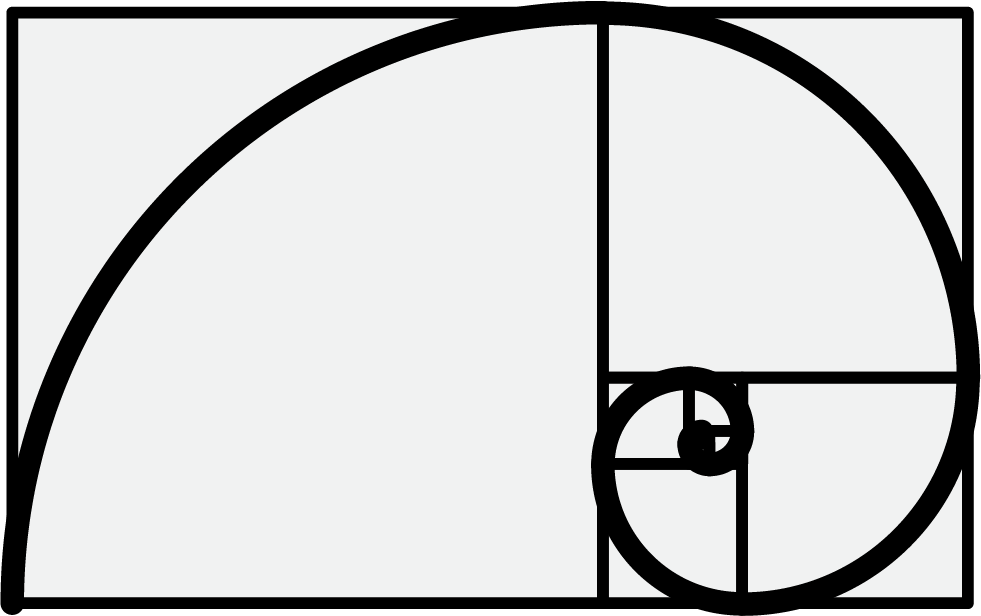
\includegraphics[height=0.75cm]{../../../AAA_template_latex_settings/pwr-control_logo_doc.png}}
\rfoot{\small Rev.~00}
% same text width as the formula sheet (17 cm)
\geometry{left=2.0cm, right=2.0cm}
\usepgfplotslibrary{groupplots}
\setcounter{tocdepth}{1}
\sisetup{per-mode=symbol,range-phrase={\text{--}},range-units=single}
\setlist{itemsep=2pt,topsep=3pt,parsep=0pt}
\setlength{\parindent}{0pt}
\setlength{\parskip}{4pt}
\allowdisplaybreaks

% --- shorthand (same as b6c_sizing_formulas.tex) ---
\newcommand{\Vdo}{V_{d0}}
\newcommand{\Vd}{V_{d}}
\newcommand{\Id}{I_{d}}
\newcommand{\Vll}{V_{2}}
\newcommand{\Xk}{X_{k}}
\newcommand{\Lk}{L_{k}}
\newcommand{\Rk}{R_{k}}
\newcommand{\uk}{u_{k}}
\newcommand{\ur}{u_{r}}
\newcommand{\Dx}{D_{x}}
\newcommand{\Dr}{D_{r}}
\newcommand{\Dt}{D_{t}}
\newcommand{\ITav}{I_{T\mathrm{(AV)}}}
\newcommand{\ITrms}{I_{T\mathrm{(RMS)}}}
\newcommand{\ITSM}{I_{TSM}}
\newcommand{\VRRM}{V_{RRM}}
\newcommand{\VRSM}{V_{RSM}}
\newcommand{\VDRM}{V_{DRM}}
\newcommand{\iit}{I^{2}t}
\newcommand{\Tj}{T_{j}}
% --- references to the formula sheet (FS), Rev. 01 numbering ---
\newcommand{\fs}[1]{\textsf{FS}\,(#1)}
\newcommand{\fsS}[1]{\textsf{FS}\,#1}
\newcommand{\fssec}[1]{\textsf{FS}\,Sec.~#1}
\newcommand{\fstab}[1]{\textsf{FS}\,Table~#1}
\newcommand{\fsfig}[1]{\textsf{FS}\,Fig.~#1}

% =============================================================
%  DOCUMENT DATA (title page: AAA_template_latex_settings/titlepage.tex)
% =============================================================
\newcommand{\DocCategory}{Technical Note}
\newcommand{\DocField}{Power Electronics and Control Systems}
\newcommand{\DocTitle}{%
	{\fontsize{20}{24}\selectfont\bfseries Six-Pulse Thyristor Bridge (B6C)} \\[16pt]
	{\fontsize{16}{20}\selectfont\bfseries Theory and Derivation of the Sizing Relations}
}
\newcommand{\DocSubtitle}{Companion to the sizing formula sheet and design path (Rev.~01)}
\newcommand{\DocAuthor}{Davide Bagnara}
\newcommand{\DocRevision}{00}
\newcommand{\DocDate}{October 2026}
\newcommand{\DocAbstract}{%
Theory companion of the sizing formula sheet \emph{Six-Pulse Thyristor Bridge (B6C) with Arm Fuses, RC Snubbers and DC LC Filter}, Rev.~01. It derives the relations the sheet quotes and explains the mechanisms behind them: the ideal six-pulse waveforms and the cosine law; where the commutation overlap comes from, the voltage lost to it and how it is compensated in the sizing and in the control; the thyristor voltage, loss, thermal and surge relations; the reverse recovery, the quantities that move the recovered charge $Q_{rr}$ and why the turn-off at $\alpha+\mu\to\SI{90}{\degree}$ is the design point; the snap-off transient of the RC snubber, its normalisation $F(\zeta_s,\chi)$, the seven sizing criteria and the bridge-level protection; the fault currents, the fuse quantities and the $I^2t$ coordination; the harmonics of the output voltage and the LC filter with its damping; and the couplings that make the sizing path iterative. The worked example of the sheet is traced step by step. Every section states which equations and steps of the sheet it supports.
}
\newcommand{\RevisionHistory}{%
	00 & October 2026 & First issue, companion of the formula sheet Rev.~01. & \DocAuthor \\
}
\newcommand{\MetaLabelA}{Project Repository}
\newcommand{\MetaValueAUrl}{https://github.com/pwr-control/repositories-documentation.git}
\newcommand{\MetaValueALabel}{repositories-documentation.git}
\newcommand{\MetaLabelB}{Calculation}
\newcommand{\MetaValueB}{Python 3 / NumPy (\texttt{b6c\_example\_calc.py}, \texttt{b6c\_theory\_figs.py})}

\begin{document}
% =============================================================
%  pwr-control LaTeX template - FRONTESPIZIO
%
%  Da richiamare come prima istruzione dopo \begin{document}:
%      \input{../../AAA_template_latex_settings/titlepage}
%
%  Il documento deve definire prima di \begin{document}:
%      \DocCategory   categoria del documento
%      \DocField      area tecnica
%      \DocTitle      titolo (una o due righe)
%      \DocSubtitle   sottotitolo
%      \DocAuthor     autore/i, separati da virgola
%      \DocRevision   numero di revisione corrente (es. 00)
%      \DocDate       data della revisione corrente
%      \DocAbstract   abstract
%      \RevisionHistory  righe della tabella di revisione, nel formato
%                        Rev. & Date & Description & Authors \\
%      \MetaLabelA \MetaValueAUrl \MetaValueALabel
%      \MetaLabelB \MetaValueB
% =============================================================

\providecommand{\DocCategory}{Technical Research Report}
\providecommand{\DocField}{Power Electronics and Control Systems}
\providecommand{\DocSubtitle}{}
\providecommand{\DocRevision}{00}
\providecommand{\DocAbstract}{}
\providecommand{\RevisionHistory}{%
	\DocRevision & \DocDate & First issue. & \DocAuthor \\
}

\titlepage

% ---- Intestazione centrata ----
\begin{center}
	{\Large\scshape \DocCategory}\\[8pt]
	{\large\scshape \DocField}
\end{center}

\vspace{30pt plus 4pt minus 14pt}
\noindent\rule{\linewidth}{0.8pt}

% ---- Titolo ----
\begin{center}
	\DocTitle
\end{center}

\vspace{4pt}
\noindent\rule{\linewidth}{2.2pt}

% ---- Sottotitolo ----
\begin{center}
	\begin{onehalfspace}
		{\large\itshape \DocSubtitle}
	\end{onehalfspace}
\end{center}

% ---- Authors / Revision / Date ----
\vspace{30pt plus 4pt minus 14pt}

\noindent
\begin{minipage}[t]{0.46\linewidth}
	\raggedright
	\textbf{Authors:}\\[2pt]
	\DocAuthor
\end{minipage}%
\hfill
\begin{minipage}[t]{0.22\linewidth}
	\centering
	\textbf{Revision:}\\[2pt]
	\DocRevision
\end{minipage}%
\hfill
\begin{minipage}[t]{0.30\linewidth}
	\raggedleft
	\textbf{Date:}\\[2pt]
	\DocDate
\end{minipage}

\vspace{10pt}
\noindent\rule{\linewidth}{0.8pt}

% ---- Abstract ----
\vspace{24pt plus 4pt minus 12pt}

\begin{center}
	\begin{minipage}{0.88\linewidth}
		\footnotesize
		\begin{onehalfspace}
			\textbf{Abstract:} \DocAbstract
		\end{onehalfspace}
	\end{minipage}
\end{center}

\vfill

% ---- Revision history ----
\begin{center}
	\begin{minipage}{0.96\linewidth}
		\centering
		{\footnotesize\scshape Revision history}\\[6pt]
		{\footnotesize
			\begin{tabular}{@{}cl>{\raggedright\arraybackslash}p{0.36\linewidth}>{\raggedright\arraybackslash}p{0.28\linewidth}@{}}
				\toprule
				\textbf{Rev.} & \textbf{Date} & \textbf{Description} & \textbf{Authors} \\
				\midrule
				\RevisionHistory
				\bottomrule
			\end{tabular}}
	\end{minipage}
\end{center}

\vspace{18pt plus 4pt minus 10pt}

% ---- Metadati in fondo ----
\noindent
\begin{tabular}{@{} r @{\quad} l @{}}
	\textsc{\MetaLabelA:} & {\href{\MetaValueAUrl}{\MetaValueALabel}} \\[3pt]
	\textsc{\MetaLabelB:} & {\MetaValueB}       \\[3pt]
\end{tabular}

% =============================================================
%  Fine frontespizio
% =============================================================
\newpage
\pagenumbering{arabic}
\setcounter{page}{1}

\tableofcontents
\newpage

\section*{Scope}
This note is the theory companion of the formula sheet \emph{Six-Pulse Thyristor Bridge (B6C) with Arm Fuses, RC Snubbers and DC LC Filter -- Sizing formula sheet and design path}, Rev.~01 \cite{fs}. The sheet quotes the sizing relations without derivation and organises them in the fourteen-step path S1--S14; this note explains where each relation comes from, which physical mechanism it describes, which assumptions it carries and why the design path has to iterate. Nothing here is needed to run the path; everything here is needed to know when the path can be trusted and how to adapt it.

The notation is that of the sheet. Equations of the sheet are cited as \fs{2.3}, its steps as \fsS{S8}, its sections, table and figure as \fssec{5}, \fstab{1}, \fsfig{2}; the numbers refer to Rev.~01. Equation numbers without prefix are those of this note. The six thyristors are numbered in firing order (Fig.~\ref{fig:bridge}): T1, T3, T5 form the common-cathode group on phases $a$, $b$, $c$ (rail $p$); T4, T6, T2 the common-anode group (rail $n$). Phase EMFs $e_a, e_b, e_c$ have peak $\hat V_{ph} = \sqrt2\,\Vll/\sqrt3$; line voltages have peak $\hat V_2 = \sqrt2\,\Vll$. The angle $\theta = \omega t$ is counted, for each commutation, from the natural commutation instant, i.e.\ the crossing of the two phase voltages involved. The worked example of the sheet (\SI{440}{V}, \SI{1000}{A}, $\uk = \SI{6}{\percent}$, \SI{1600}{V} class) is used throughout for orders of magnitude; its numbers come from \texttt{b6c\_example\_calc.py}, the figure data of this note from \texttt{b6c\_theory\_figs.py}.

\begin{table}[htb]
\centering\footnotesize
\caption{Reading guide: where each part of the sheet is derived.}
\label{tab:map}
\begin{tabular}{@{}p{7.2cm}p{6.8cm}p{1.8cm}@{}}
\toprule
This note & Sheet & Steps \\
\midrule
Sec.~\ref{sec:ideal} Ideal bridge: $\Vdo$, $\cos\alpha$ law, currents, transformer rating & \fssec{2}, \fssec{8}: \fs{2.1}, \fs{2.7}, \fs{8.1}, \fs{8.2} & S2, S3, S14 \\
Sec.~\ref{sec:overlap} Commutation, overlap, drops, their compensation, power factor & \fssec{2}, \fssec{3}: \fs{2.2}--\fs{2.6}, \fs{3.1}--\fs{3.6} & S2--S4, S7 \\
Sec.~\ref{sec:thy} Thyristor voltage, losses, thermal chain, surge, $\iit$ & \fssec{4}: \fs{4.1}--\fs{4.8} & S5--S7 \\
Sec.~\ref{sec:rr} Reverse recovery: $Q_{rr}$, what moves it, the turn-off point of the B6C & \fssec{5.2}: \fs{5.1}--\fs{5.3} & S7, S8 \\
Sec.~\ref{sec:snub} RC snubber: snap-off transient, $F(\zeta_s,\chi)$, criteria C1--C7, bridge level & \fssec{5}: \fs{5.4}--\fs{5.15}, \fstab{1}, \fsfig{2} & S5, S8 \\
Sec.~\ref{sec:fuse} Fault currents, fuse quantities, $\iit$ coordination & \fssec{6}: \fs{6.1}--\fs{6.13} & S9--S11 \\
Sec.~\ref{sec:filter} Output voltage harmonics, LC filter, damping, ratings & \fssec{7}: \fs{7.1}--\fs{7.17} & S12, S13 \\
Sec.~\ref{sec:loops} Why the path iterates & \fssec{1}, \fsfig{1} & all \\
Sec.~\ref{sec:example} The worked example traced & \fssec{10} & all \\
\bottomrule
\end{tabular}
\end{table}

%=====================================================================
\section{The ideal bridge}\label{sec:ideal}
\subsection{Topology and conduction sequence}
Figure~\ref{fig:bridge} shows the circuit the sheet sizes. The transformer (with the line reactor and the grid, if any) is reduced to three EMFs behind one commutation inductance $\Lk$ and resistance $\Rk$ per phase, referred to the bridge terminals. Each arm has a thyristor, a fuse in series and an RC snubber across the thyristor; the output feeds an LC filter and the load. With ideal commutation ($\Lk = 0$) and continuous DC current, exactly one device of each group conducts at any instant: in the common-cathode group the device connected to the most positive phase, in the common-anode group the one connected to the most negative phase. The output voltage is therefore the line-to-line voltage between those two phases, and it changes every \SI{60}{\degree}: six segments per cycle, hence six-pulse. Each thyristor conducts for \SI{120}{\degree}; the firings follow the order T1, T2, \ldots, T6 at \SI{60}{\degree} intervals, so that two devices (one per group) are always on and the pairs (T1,T2), (T2,T3), \ldots\ conduct for \SI{60}{\degree} each.

\begin{figure}[htb]
\centering
\begin{tikzpicture}[x=0.95cm,y=0.95cm,line width=0.6pt,>=latex]
% thyristor: anode at bottom, cathode at top (current flows upwards, from n to p), gate to the left. #1 label, #2 centre
\newcommand{\thy}[2]{%
  \begin{scope}[shift={#2}]
    \draw (0,0.55) -- (0,0.1);
    \draw (-0.25,0.1) -- (0.25,0.1);
    \draw[fill=white] (-0.25,-0.28) -- (0.25,-0.28) -- (0,0.1) -- cycle;
    \draw (0,-0.28) -- (0,-0.55);
    \draw (-0.22,0.1) -- (-0.45,0.32);
    \node[font=\scriptsize,anchor=east] at (-0.3,-0.2) {#1};
  \end{scope}}
% fuse: vertical, #1 centre
\newcommand{\fuse}[1]{%
  \begin{scope}[shift={#1}]
    \draw (0,0.35) -- (0,-0.35);
    \draw[fill=white] (-0.14,0.25) rectangle (0.14,-0.25);
  \end{scope}}
% RC snubber across the thyristor: #1 x of the arm, #2 y of the thyristor centre
\newcommand{\snub}[2]{%
  \begin{scope}[shift={(#1,#2)}]
    \draw (0,0.55) -- (0.75,0.55) -- (0.75,0.3);
    \draw[fill=white] (0.65,0.3) rectangle (0.85,-0.05);
    \draw (0.75,-0.05) -- (0.75,-0.22);
    \draw (0.6,-0.22) -- (0.9,-0.22);
    \draw (0.6,-0.32) -- (0.9,-0.32);
    \draw (0.75,-0.32) -- (0.75,-0.55) -- (0,-0.55);
    \node[font=\tiny,anchor=west] at (0.88,0.13) {$R_s$};
    \node[font=\tiny,anchor=west] at (0.92,-0.27) {$C_s$};
  \end{scope}}
% rails
\draw (0.6,3.0) -- (9.2,3.0) node[right,font=\small] {$p$};
\draw (0.6,-3.0) -- (9.2,-3.0) node[right,font=\small] {$n$};
% arms at x = 1.5, 4.0, 6.5; AC connection heights 0.4, 0, -0.4
\foreach \x/\tu/\tl/\ya in {1.5/T1/T4/0.5, 4.0/T3/T6/0, 6.5/T5/T2/-0.5}{
  \draw (\x,3.0) -- (\x,2.65);
  \fuse{(\x,2.3)}
  \draw (\x,1.95) -- (\x,1.75);
  \thy{\tu}{(\x,1.2)}
  \draw (\x,0.65) -- (\x,-0.65);
  \snub{\x}{1.2}
  \thy{\tl}{(\x,-1.2)}
  \snub{\x}{-1.2}
  \draw (\x,-1.75) -- (\x,-1.95);
  \fuse{(\x,-2.3)}
  \draw (\x,-2.65) -- (\x,-3.0);
  \fill (\x,\ya) circle (1.3pt);
}
% AC feeders: phase a at y = 0.4, b at 0, c at -0.4 (crossings without dot are not connected)
\foreach \y/\ph/\xe in {0.5/a/1.5, 0/b/4.0, -0.5/c/6.5}{
  \draw (-0.4,\y) -- (\xe,\y);
  \draw[fill=white] (-1.0,\y+0.1) rectangle (-0.4,\y-0.1);
  \draw (-1.0,\y) -- (-1.2,\y);
  \draw (-1.8,\y) arc (180:0:0.1) arc (180:0:0.1) arc (180:0:0.1);
  \draw (-1.8,\y) -- (-2.12,\y);
  \draw (-2.3,\y) circle (0.18);
  \node[font=\tiny] at (-2.3,\y) {$e_\ph$};
  \draw (-2.48,\y) -- (-2.9,\y);
}
\node[font=\scriptsize,above] at (-0.7,0.6) {$\Rk$};
\node[font=\scriptsize,above] at (-1.5,0.65) {$\Lk$};
\node[font=\scriptsize,above] at (0.3,0.52) {$a$};
\node[font=\scriptsize,above] at (2.6,0.02) {$b$};
\node[font=\scriptsize,above] at (5.1,-0.48) {$c$};
\draw (-2.9,0.5) -- (-2.9,-0.5);
\fill (-2.9,0) circle (1.2pt);
\node[font=\scriptsize,left] at (-2.9,0) {$N$};
% DC side: L, C, load
\draw (9.2,3.0) -- (9.6,3.0);
\draw[fill=white] (9.6,3.12) rectangle (10.2,2.88);
\draw (10.2,3.0) -- (11.4,3.0) -- (11.4,0.25);
\draw (11.1,0.25) -- (11.7,0.25);
\draw (11.1,0.05) -- (11.7,0.05);
\draw (11.4,0.05) -- (11.4,-3.0) -- (9.2,-3.0);
\draw (11.4,3.0) -- (12.6,3.0) -- (12.6,0.6);
\draw[fill=white] (12.45,0.6) rectangle (12.75,-0.6);
\draw (12.6,-0.6) -- (12.6,-3.0) -- (11.4,-3.0);
\fill (11.4,3.0) circle (1.2pt);
\fill (11.4,-3.0) circle (1.2pt);
\node[font=\scriptsize,above] at (9.9,3.12) {$L$};
\node[font=\scriptsize,right] at (11.7,0.15) {$C$};
\node[font=\scriptsize,right] at (12.75,0) {load};
\draw[->] (10.4,3.3) -- (11.0,3.3) node[midway,above,font=\scriptsize] {$\Id$};
\draw[<->] (13.3,2.6) -- (13.3,-2.6) node[midway,right,font=\scriptsize] {$\Vd$};
\end{tikzpicture}
\caption{B6C with arm fuses, RC snubbers across the thyristors and LC output filter. The AC source is the Th\'evenin equivalent seen from the bridge terminals: EMF, commutation inductance $\Lk$ and resistance $\Rk$ per phase. Crossing wires are not connected.}
\label{fig:bridge}
\end{figure}

\subsection{No-load voltage and the cosine law}
Take the $\SI{60}{\degree}$ segment during which the output follows one line voltage, and count $\theta$ from the centre of the segment, where that line voltage has its peak $\hat V_2 = \sqrt2\,\Vll$. With ideal commutation and firing at the natural instant ($\alpha = 0$) the segment runs from $-\pi/6$ to $+\pi/6$ and the mean output voltage is
\begin{equation}
\Vdo = \frac{1}{\pi/3}\int_{-\pi/6}^{\pi/6}\hat V_2\cos\theta\,d\theta = \frac{3}{\pi}\hat V_2\cdot2\sin\frac{\pi}{6} = \frac{3}{\pi}\sqrt2\,\Vll = 1.350\,\Vll ,
\label{eq:Vdo}
\end{equation}
which is \fs{2.1}. A firing delay $\alpha$ shifts the segment to $(-\pi/6+\alpha,\ \pi/6+\alpha)$ without changing its length, because the next firing is delayed by the same $\alpha$:
\begin{equation}
\Vd(\alpha) = \frac{3}{\pi}\int_{-\pi/6+\alpha}^{\pi/6+\alpha}\hat V_2\cos\theta\,d\theta = \frac{3}{\pi}\hat V_2\left[\sin\!\left(\tfrac{\pi}{6}+\alpha\right)-\sin\!\left(\alpha-\tfrac{\pi}{6}\right)\right] = \frac{3}{\pi}\hat V_2\cdot2\cos\alpha\sin\frac{\pi}{6} = \Vdo\cos\alpha .
\label{eq:cosalpha}
\end{equation}
Two conditions are built into \eqref{eq:cosalpha}. First, the thyristor can be fired only when it is forward biased, i.e.\ after its phase voltage has exceeded that of the conducting phase; the delay is therefore counted from the natural crossing and $0 \le \alpha < \pi$. Second, the DC current never falls to zero (continuous conduction, Sec.~\ref{sec:lmin}); in discontinuous conduction the output follows the line voltage only while current flows, the mean rises above $\Vdo\cos\alpha$ and the control gain changes. For $\alpha > \SI{90}{\degree}$ the mean is negative: with a current that can only flow in one direction, power flows back to the grid (inverter operation), which the unipolar filter capacitor of this design excludes (\fs{3.5} and Sec.~\ref{sec:gamma}).

\subsection{Currents, harmonics and transformer rating}\label{sec:currents}
With smooth $\Id$ each thyristor carries a rectangular block of amplitude $\Id$ and width \SI{120}{\degree}:
\begin{equation}
\ITav = \frac{1}{2\pi}\int_0^{2\pi/3}\Id\,d\theta = \frac{\Id}{3}, \qquad
\ITrms = \sqrt{\frac{1}{2\pi}\int_0^{2\pi/3}\Id^2\,d\theta} = \frac{\Id}{\sqrt3}, \qquad
\frac{\ITrms}{\ITav} = \sqrt3 ,
\label{eq:ITderiv}
\end{equation}
which is \fs{4.3}. A secondary phase carries $+\Id$ for \SI{120}{\degree} (through its upper device) and $-\Id$ for \SI{120}{\degree} (through its lower device), hence $I_2 = \sqrt{2/3}\,\Id$ in \fs{2.7} and \fs{8.1}. The Fourier series of this quasi-square wave, odd about the centre of the positive block, has only sine terms,
\begin{equation}
b_h = \frac{2}{\pi}\int_{\pi/6}^{5\pi/6}\Id\sin h\theta\,d\theta = \frac{2\Id}{h\pi}\left[\cos\frac{h\pi}{6}-\cos\frac{5h\pi}{6}\right] =
\begin{cases}
\pm\dfrac{2\sqrt3}{h\pi}\Id & h = 6k\pm1,\\[6pt]
0 & h \ \text{even or multiple of 3},
\end{cases}
\label{eq:fourierI}
\end{equation}
so the fundamental is $I_1 = b_1/\sqrt2 = (\sqrt6/\pi)\Id = 0.780\,\Id$ and every characteristic harmonic obeys $I_h = I_1/h$ \fs{8.1}. The triplen harmonics cancel because the three blocks are \SI{120}{\degree} apart, the even ones because of the half-wave symmetry; this is why a six-pulse bridge injects $5, 7, 11, 13, \ldots$ and nothing else as long as the firing is symmetric and the grid balanced. The total harmonic distortion follows from the ratio of the RMS values,
\begin{equation}
THD_i = \sqrt{\frac{I_2^2}{I_1^2}-1} = \sqrt{\frac{2/3}{6/\pi^2}-1} = \sqrt{\frac{\pi^2}{9}-1} = 0.311 ,
\qquad \frac{I_1}{I_2} = \frac{3}{\pi} = 0.955 ,
\label{eq:THDderiv}
\end{equation}
\fs{8.2}; $3/\pi$ is the distortion factor that turns the displacement factor $\cos\varphi_1$ into the power factor $\lambda$ of \fs{3.3}. The transformer rating uses the RMS secondary current, not the mean of the output:
\begin{equation}
S_T = \sqrt3\,\Vll I_2 = \sqrt3\cdot\frac{\pi}{3\sqrt2}\Vdo\cdot\sqrt{\frac23}\,\Id = \frac{\pi}{3}\Vdo\Id = 1.047\,P_{d0} ,
\label{eq:STderiv}
\end{equation}
\fs{2.7}. The \SI{4.7}{\percent} excess over the DC power is the price of the harmonic content of the winding current. In the B6 connection the secondary current has no DC component, so primary and secondary windings have the same rating (unlike the three-pulse M3, where the DC magnetisation forces a larger core). Overlap rounds the edges of the current blocks and reduces the high-order harmonics; a ripple current on the DC side adds mainly to the 5th and 7th (Sec.~\ref{sec:gridh}).

%=====================================================================
\section{Commutation and overlap}\label{sec:overlap}
\subsection{Where the overlap comes from}
The current in an inductance cannot jump. When T3 is fired while T1 carries $\Id$, the current cannot leave phase $a$ and enter phase $b$ instantaneously: for a while both devices conduct, the two phases are short-circuited through the bridge, and the line voltage $e_b - e_a$ drives the transfer of current around the loop $\Lk$--T1--T3--$\Lk$ (Fig.~\ref{fig:commloop}). Writing the two branch equations with $\Rk$ neglected, the common cathode voltage $v_p$ and the constraint $i_a + i_b = \Id$ (the DC inductance holds $\Id$ constant over the few hundred microseconds of a commutation),
\begin{equation}
e_a - \Lk\frac{di_a}{dt} = v_p = e_b - \Lk\frac{di_b}{dt}, \qquad \frac{di_a}{dt} = -\frac{di_b}{dt}
\quad\Rightarrow\quad
e_b - e_a = 2\Lk\frac{di_b}{dt}, \qquad v_p = \frac{e_a+e_b}{2} .
\label{eq:commKVL}
\end{equation}
Two facts follow at once: the loop inductance is $2\Lk$ (both phases are in the path, which is why $2\Lk$ appears in every turn-off and snubber formula of the sheet), and during the overlap the rail is held at the mean of the two phase voltages, not at the incoming one. Counting $\theta$ from the natural crossing, $e_b - e_a = \hat V_2\sin\theta$ and integration from the firing instant $\theta = \alpha$ gives the incoming current
\begin{equation}
i_b(\theta) = \frac{\hat V_2}{2\omega\Lk}\left(\cos\alpha - \cos\theta\right), \qquad \alpha\le\theta\le\alpha+\mu .
\label{eq:ib}
\end{equation}
The commutation ends when $i_b$ reaches $\Id$, which defines the overlap angle $\mu$:
\begin{equation}
\cos\alpha - \cos(\alpha+\mu) = \frac{2\omega\Lk\Id}{\hat V_2} = \frac{\sqrt2\,\Xk\Id}{\Vll} ,
\label{eq:muderiv}
\end{equation}
which is \fs{3.1}. The right-hand side is a property of the installation (reactance and current); the left-hand side says how much of the line voltage is available to push the current: near $\alpha = 0$ the driving voltage starts from zero and $\mu$ is largest, around $\alpha = \SI{90}{\degree}$ the voltage is at its peak and $\mu$ is smallest, towards $\alpha\to\SI{180}{\degree}$ it shrinks again, which is the inverter-mode problem of Sec.~\ref{sec:gamma}. In the example $\mu$ goes from \SI{13.3}{\degree} at $\alpha = \SI{10}{\degree}$ to \SI{5.0}{\degree} at \SI{36}{\degree} (\fsS{S4}).

\begin{figure}[htb]
\centering
\begin{tikzpicture}[x=1cm,y=1cm,line width=0.6pt,>=latex]
% two phases, two Lk, two thyristors to a common cathode, DC current source
\foreach \y/\ph/\T in {1.2/a/T1, -1.2/b/T3}{
  \draw (0,\y) circle (0.22);
  \node[font=\scriptsize,left] at (-0.25,\y) {$e_\ph$};
  \draw (0.22,\y) -- (0.7,\y);
  \draw (0.7,\y) \foreach \i in {0,1,2,3} { arc (180:0:0.1) };
  \node[font=\scriptsize,above] at (1.1,\y+0.12) {$\Lk$};
  \draw (1.5,\y) -- (2.6,\y);
  % thyristor horizontal: anode left
  \draw[fill=white] (2.6,\y+0.22) -- (2.6,\y-0.22) -- (3.0,\y) -- cycle;
  \draw (3.0,\y+0.22) -- (3.0,\y-0.22);
  \draw (3.0,\y) -- (4.2,\y);
  \node[font=\scriptsize,above] at (2.8,\y+0.25) {\T};
}
\draw (-0.22,1.2) -- (-0.6,1.2) -- (-0.6,-1.2) -- (-0.22,-1.2);
\draw (4.2,1.2) -- (4.2,-1.2);
\fill (4.2,0) circle (1.2pt);
\node[font=\scriptsize,above right] at (4.2,0.05) {$p$};
% current source to the right, returning to N
\draw (4.2,0) -- (5.4,0);
\draw (5.4,0) circle (0.3);
\draw[->] (5.4,0.3) -- (5.4,-0.3);
\node[font=\scriptsize,right] at (5.75,0) {$\Id$};
\draw (5.4,-0.3) -- (5.4,-2.0) -- (-0.6,-2.0) -- (-0.6,-1.2);
\node[font=\scriptsize,below] at (2.4,-2.0) {return through the conducting device of the other group};
% currents
\draw[->,red!70!black] (1.8,1.5) -- (2.4,1.5) node[midway,above,font=\scriptsize] {$i_a = \Id - i_b$};
\draw[->,blue!70!black] (1.8,-0.9) -- (2.4,-0.9) node[midway,above,font=\scriptsize] {$i_b$};
% loop arrow
\draw[->,thick,gray] (1.0,0.6) arc (120:-120:0.6) ;
\node[font=\scriptsize,gray] at (2.1,0) {$e_b - e_a = 2\Lk\,di_b/dt$};
\end{tikzpicture}
\caption{Commutation loop T1$\to$T3. Both phase inductances are in the loop; the rail $p$ sits at the mean of $e_a$ and $e_b$ while both devices conduct.}
\label{fig:commloop}
\end{figure}

\subsection{The voltage lost to commutation}\label{sec:Dx}
While the rail is held at $(e_a+e_b)/2$ instead of $e_b$, the output loses $(e_b-e_a)/2 = \Lk\,di_b/dt$. The volt-seconds lost in one commutation are therefore
\begin{equation}
\int_{t_\alpha}^{t_{\alpha+\mu}}\frac{e_b-e_a}{2}\,dt = \Lk\int_0^{\Id}di_b = \Lk\Id ,
\label{eq:voltsec}
\end{equation}
independent of $\alpha$ and of the shape of the voltage during the overlap. There are six commutations per cycle, one every $T/6$, so the mean voltage lost is
\begin{equation}
\Dx = \frac{\Lk\Id}{T/6} = 6f\Lk\Id = \frac{3}{\pi}\omega\Lk\Id = \frac{3}{\pi}\Xk\Id ,
\label{eq:Dxderiv}
\end{equation}
which is \fs{2.3}. The output characteristic $\Vd = \Vdo\cos\alpha - (3/\pi)\Xk\Id$ looks like a source with an internal resistance $R_c = (3/\pi)\Xk$, but $R_c$ dissipates nothing: the lost volt-seconds are reactive power exchanged with the AC side, not heat. The same result can be written with \eqref{eq:muderiv}, since $\Dx = \tfrac{3}{\pi}\cdot\tfrac{\hat V_2}{2}[\cos\alpha-\cos(\alpha+\mu)] = \tfrac{\Vdo}{2}[\cos\alpha-\cos(\alpha+\mu)]$:
\begin{equation}
\Vd = \Vdo\,\frac{\cos\alpha+\cos(\alpha+\mu)}{2} - \Dr - \Dt ,
\label{eq:Vdmu}
\end{equation}
the form that makes the power factor of Sec.~\ref{sec:pf} immediate. Figure~\ref{fig:waves} shows the rail voltages, the output voltage with its notches, and the rounded phase current, computed with the model of this section for $\alpha = \SI{30}{\degree}$, $\mu = \SI{15}{\degree}$.

The resistive drop is $\Dr = 2\Rk\Id$ \fs{2.4} because, outside the overlaps, the DC current flows through two phases in series; the device drop $\Dt = 2(V_{T0}+r_T\Id)$ \fs{2.5} for the same reason. The per-unit forms of the sheet follow from the transformer definitions $\Xk = \uk\Vll^2/S_T$, $\Rk = \ur\Vll^2/S_T$ and from \eqref{eq:Vdo}, \eqref{eq:STderiv}:
\begin{equation}
d_x = \frac{\Dx}{\Vdo} = \frac{3}{\pi}\,\frac{\uk\Vll^2\Id}{S_T\Vdo} = \frac{3}{\pi}\,\frac{3}{\pi}\,\frac{\uk\Vll^2}{\Vdo^2} = \frac{9}{\pi^2}\cdot\frac{\pi^2}{18}\,\uk = \frac{\uk}{2}, \qquad
d_r = \frac{2\Rk\Id}{\Vdo} = \frac{2\cdot3}{\pi}\cdot\frac{\pi^2}{18}\,\ur = \frac{\pi}{3}\ur ,
\label{eq:dxdr}
\end{equation}
using $\Vll^2/\Vdo^2 = \pi^2/18$. Half of the transformer short-circuit voltage is lost to commutation at rated current, whatever the voltage level: this is the first-guess $d_x = \uk/2$ of \fsS{S2}. ($\ur$ is defined from the copper losses, $3\Rk I_2^2 = \ur S_T$, and $2\Rk\Id^2 = 3\Rk I_2^2$ with $I_2^2 = \tfrac23\Id^2$: the resistive drop is exactly the winding loss divided by $\Id$.)

\begin{figure}[htb]
\centering
\begin{tikzpicture}
\begin{groupplot}[group style={group size=1 by 3, vertical sep=9mm},
  width=0.76\textwidth, height=0.27\textwidth, xmin=0, xmax=360, xtick={0,60,...,360},
  grid=major, grid style={gray!25}, every axis plot/.append style={thick},
  legend pos=outer north east, legend style={font=\scriptsize}, legend cell align=left,
  tick label style={font=\scriptsize}, label style={font=\scriptsize}]
\nextgroupplot[ylabel={$v/\hat V_{ph}$}, ymin=-1.15, ymax=1.15]
\addplot[gray!60, thin, domain=0:360, samples=181] {sin(x)};
\addplot[gray!60, thin, domain=0:360, samples=181] {sin(x-120)};
\addplot[gray!60, thin, domain=0:360, samples=181] {sin(x+120)};
\addplot[red!70!black] coordinates {(0.0,0.866) (1.0,0.857) (2.0,0.848) (3.0,0.839) (4.0,0.829) (5.0,0.819) (6.0,0.809) (7.0,0.799) (8.0,0.788) (9.0,0.777) (10.0,0.766) (11.0,0.755) (12.0,0.743) (13.0,0.731) (14.0,0.719) (15.0,0.707) (16.0,0.695) (17.0,0.682) (18.0,0.669) (19.0,0.656) (20.0,0.643) (21.0,0.629) (22.0,0.616) (23.0,0.602) (24.0,0.588) (25.0,0.574) (26.0,0.559) (27.0,0.545) (28.0,0.530) (29.0,0.515) (30.0,0.500) (31.0,0.485) (32.0,0.469) (33.0,0.454) (34.0,0.438) (35.0,0.423) (36.0,0.407) (37.0,0.391) (38.0,0.375) (39.0,0.358) (40.0,0.342) (41.0,0.326) (42.0,0.309) (43.0,0.292) (44.0,0.276) (45.0,0.259) (46.0,0.242) (47.0,0.225) (48.0,0.208) (49.0,0.191) (50.0,0.174) (51.0,0.156) (52.0,0.139) (53.0,0.122) (54.0,0.105) (55.0,0.087) (56.0,0.070) (57.0,0.052) (58.0,0.035) (59.0,0.017) (60.0,0.433) (61.0,0.429) (62.0,0.424) (63.0,0.419) (64.0,0.415) (65.0,0.410) (66.0,0.405) (67.0,0.399) (68.0,0.394) (69.0,0.389) (70.0,0.383) (71.0,0.377) (72.0,0.372) (73.0,0.366) (74.0,0.360) (75.0,0.966) (76.0,0.970) (77.0,0.974) (78.0,0.978) (79.0,0.982) (80.0,0.985) (81.0,0.988) (82.0,0.990) (83.0,0.993) (84.0,0.995) (85.0,0.996) (86.0,0.998) (87.0,0.999) (88.0,0.999) (89.0,1.000) (90.0,1.000) (91.0,1.000) (92.0,0.999) (93.0,0.999) (94.0,0.998) (95.0,0.996) (96.0,0.995) (97.0,0.993) (98.0,0.990) (99.0,0.988) (100.0,0.985) (101.0,0.982) (102.0,0.978) (103.0,0.974) (104.0,0.970) (105.0,0.966) (106.0,0.961) (107.0,0.956) (108.0,0.951) (109.0,0.946) (110.0,0.940) (111.0,0.934) (112.0,0.927) (113.0,0.921) (114.0,0.914) (115.0,0.906) (116.0,0.899) (117.0,0.891) (118.0,0.883) (119.0,0.875) (120.0,0.866) (121.0,0.857) (122.0,0.848) (123.0,0.839) (124.0,0.829) (125.0,0.819) (126.0,0.809) (127.0,0.799) (128.0,0.788) (129.0,0.777) (130.0,0.766) (131.0,0.755) (132.0,0.743) (133.0,0.731) (134.0,0.719) (135.0,0.707) (136.0,0.695) (137.0,0.682) (138.0,0.669) (139.0,0.656) (140.0,0.643) (141.0,0.629) (142.0,0.616) (143.0,0.602) (144.0,0.588) (145.0,0.574) (146.0,0.559) (147.0,0.545) (148.0,0.530) (149.0,0.515) (150.0,0.500) (151.0,0.485) (152.0,0.469) (153.0,0.454) (154.0,0.438) (155.0,0.423) (156.0,0.407) (157.0,0.391) (158.0,0.375) (159.0,0.358) (160.0,0.342) (161.0,0.326) (162.0,0.309) (163.0,0.292) (164.0,0.276) (165.0,0.259) (166.0,0.242) (167.0,0.225) (168.0,0.208) (169.0,0.191) (170.0,0.174) (171.0,0.156) (172.0,0.139) (173.0,0.122) (174.0,0.105) (175.0,0.087) (176.0,0.070) (177.0,0.052) (178.0,0.035) (179.0,0.017) (180.0,0.433) (181.0,0.429) (182.0,0.424) (183.0,0.419) (184.0,0.415) (185.0,0.410) (186.0,0.405) (187.0,0.399) (188.0,0.394) (189.0,0.389) (190.0,0.383) (191.0,0.377) (192.0,0.372) (193.0,0.366) (194.0,0.360) (195.0,0.966) (196.0,0.970) (197.0,0.974) (198.0,0.978) (199.0,0.982) (200.0,0.985) (201.0,0.988) (202.0,0.990) (203.0,0.993) (204.0,0.995) (205.0,0.996) (206.0,0.998) (207.0,0.999) (208.0,0.999) (209.0,1.000) (210.0,1.000) (211.0,1.000) (212.0,0.999) (213.0,0.999) (214.0,0.998) (215.0,0.996) (216.0,0.995) (217.0,0.993) (218.0,0.990) (219.0,0.988) (220.0,0.985) (221.0,0.982) (222.0,0.978) (223.0,0.974) (224.0,0.970) (225.0,0.966) (226.0,0.961) (227.0,0.956) (228.0,0.951) (229.0,0.946) (230.0,0.940) (231.0,0.934) (232.0,0.927) (233.0,0.921) (234.0,0.914) (235.0,0.906) (236.0,0.899) (237.0,0.891) (238.0,0.883) (239.0,0.875) (240.0,0.866) (241.0,0.857) (242.0,0.848) (243.0,0.839) (244.0,0.829) (245.0,0.819) (246.0,0.809) (247.0,0.799) (248.0,0.788) (249.0,0.777) (250.0,0.766) (251.0,0.755) (252.0,0.743) (253.0,0.731) (254.0,0.719) (255.0,0.707) (256.0,0.695) (257.0,0.682) (258.0,0.669) (259.0,0.656) (260.0,0.643) (261.0,0.629) (262.0,0.616) (263.0,0.602) (264.0,0.588) (265.0,0.574) (266.0,0.559) (267.0,0.545) (268.0,0.530) (269.0,0.515) (270.0,0.500) (271.0,0.485) (272.0,0.469) (273.0,0.454) (274.0,0.438) (275.0,0.423) (276.0,0.407) (277.0,0.391) (278.0,0.375) (279.0,0.358) (280.0,0.342) (281.0,0.326) (282.0,0.309) (283.0,0.292) (284.0,0.276) (285.0,0.259) (286.0,0.242) (287.0,0.225) (288.0,0.208) (289.0,0.191) (290.0,0.174) (291.0,0.156) (292.0,0.139) (293.0,0.122) (294.0,0.105) (295.0,0.087) (296.0,0.070) (297.0,0.052) (298.0,0.035) (299.0,0.017) (300.0,0.433) (301.0,0.429) (302.0,0.424) (303.0,0.419) (304.0,0.415) (305.0,0.410) (306.0,0.405) (307.0,0.399) (308.0,0.394) (309.0,0.389) (310.0,0.383) (311.0,0.377) (312.0,0.372) (313.0,0.366) (314.0,0.360) (315.0,0.966) (316.0,0.970) (317.0,0.974) (318.0,0.978) (319.0,0.982) (320.0,0.985) (321.0,0.988) (322.0,0.990) (323.0,0.993) (324.0,0.995) (325.0,0.996) (326.0,0.998) (327.0,0.999) (328.0,0.999) (329.0,1.000) (330.0,1.000) (331.0,1.000) (332.0,0.999) (333.0,0.999) (334.0,0.998) (335.0,0.996) (336.0,0.995) (337.0,0.993) (338.0,0.990) (339.0,0.988) (340.0,0.985) (341.0,0.982) (342.0,0.978) (343.0,0.974) (344.0,0.970) (345.0,0.966) (346.0,0.961) (347.0,0.956) (348.0,0.951) (349.0,0.946) (350.0,0.940) (351.0,0.934) (352.0,0.927) (353.0,0.921) (354.0,0.914) (355.0,0.906) (356.0,0.899) (357.0,0.891) (358.0,0.883) (359.0,0.875) (360.0,0.866)};
\addplot[blue!70!black] coordinates {(0.0,-0.433) (1.0,-0.429) (2.0,-0.424) (3.0,-0.419) (4.0,-0.415) (5.0,-0.410) (6.0,-0.405) (7.0,-0.399) (8.0,-0.394) (9.0,-0.389) (10.0,-0.383) (11.0,-0.377) (12.0,-0.372) (13.0,-0.366) (14.0,-0.360) (15.0,-0.966) (16.0,-0.970) (17.0,-0.974) (18.0,-0.978) (19.0,-0.982) (20.0,-0.985) (21.0,-0.988) (22.0,-0.990) (23.0,-0.993) (24.0,-0.995) (25.0,-0.996) (26.0,-0.998) (27.0,-0.999) (28.0,-0.999) (29.0,-1.000) (30.0,-1.000) (31.0,-1.000) (32.0,-0.999) (33.0,-0.999) (34.0,-0.998) (35.0,-0.996) (36.0,-0.995) (37.0,-0.993) (38.0,-0.990) (39.0,-0.988) (40.0,-0.985) (41.0,-0.982) (42.0,-0.978) (43.0,-0.974) (44.0,-0.970) (45.0,-0.966) (46.0,-0.961) (47.0,-0.956) (48.0,-0.951) (49.0,-0.946) (50.0,-0.940) (51.0,-0.934) (52.0,-0.927) (53.0,-0.921) (54.0,-0.914) (55.0,-0.906) (56.0,-0.899) (57.0,-0.891) (58.0,-0.883) (59.0,-0.875) (60.0,-0.866) (61.0,-0.857) (62.0,-0.848) (63.0,-0.839) (64.0,-0.829) (65.0,-0.819) (66.0,-0.809) (67.0,-0.799) (68.0,-0.788) (69.0,-0.777) (70.0,-0.766) (71.0,-0.755) (72.0,-0.743) (73.0,-0.731) (74.0,-0.719) (75.0,-0.707) (76.0,-0.695) (77.0,-0.682) (78.0,-0.669) (79.0,-0.656) (80.0,-0.643) (81.0,-0.629) (82.0,-0.616) (83.0,-0.602) (84.0,-0.588) (85.0,-0.574) (86.0,-0.559) (87.0,-0.545) (88.0,-0.530) (89.0,-0.515) (90.0,-0.500) (91.0,-0.485) (92.0,-0.469) (93.0,-0.454) (94.0,-0.438) (95.0,-0.423) (96.0,-0.407) (97.0,-0.391) (98.0,-0.375) (99.0,-0.358) (100.0,-0.342) (101.0,-0.326) (102.0,-0.309) (103.0,-0.292) (104.0,-0.276) (105.0,-0.259) (106.0,-0.242) (107.0,-0.225) (108.0,-0.208) (109.0,-0.191) (110.0,-0.174) (111.0,-0.156) (112.0,-0.139) (113.0,-0.122) (114.0,-0.105) (115.0,-0.087) (116.0,-0.070) (117.0,-0.052) (118.0,-0.035) (119.0,-0.017) (120.0,-0.433) (121.0,-0.429) (122.0,-0.424) (123.0,-0.419) (124.0,-0.415) (125.0,-0.410) (126.0,-0.405) (127.0,-0.399) (128.0,-0.394) (129.0,-0.389) (130.0,-0.383) (131.0,-0.377) (132.0,-0.372) (133.0,-0.366) (134.0,-0.360) (135.0,-0.966) (136.0,-0.970) (137.0,-0.974) (138.0,-0.978) (139.0,-0.982) (140.0,-0.985) (141.0,-0.988) (142.0,-0.990) (143.0,-0.993) (144.0,-0.995) (145.0,-0.996) (146.0,-0.998) (147.0,-0.999) (148.0,-0.999) (149.0,-1.000) (150.0,-1.000) (151.0,-1.000) (152.0,-0.999) (153.0,-0.999) (154.0,-0.998) (155.0,-0.996) (156.0,-0.995) (157.0,-0.993) (158.0,-0.990) (159.0,-0.988) (160.0,-0.985) (161.0,-0.982) (162.0,-0.978) (163.0,-0.974) (164.0,-0.970) (165.0,-0.966) (166.0,-0.961) (167.0,-0.956) (168.0,-0.951) (169.0,-0.946) (170.0,-0.940) (171.0,-0.934) (172.0,-0.927) (173.0,-0.921) (174.0,-0.914) (175.0,-0.906) (176.0,-0.899) (177.0,-0.891) (178.0,-0.883) (179.0,-0.875) (180.0,-0.866) (181.0,-0.857) (182.0,-0.848) (183.0,-0.839) (184.0,-0.829) (185.0,-0.819) (186.0,-0.809) (187.0,-0.799) (188.0,-0.788) (189.0,-0.777) (190.0,-0.766) (191.0,-0.755) (192.0,-0.743) (193.0,-0.731) (194.0,-0.719) (195.0,-0.707) (196.0,-0.695) (197.0,-0.682) (198.0,-0.669) (199.0,-0.656) (200.0,-0.643) (201.0,-0.629) (202.0,-0.616) (203.0,-0.602) (204.0,-0.588) (205.0,-0.574) (206.0,-0.559) (207.0,-0.545) (208.0,-0.530) (209.0,-0.515) (210.0,-0.500) (211.0,-0.485) (212.0,-0.469) (213.0,-0.454) (214.0,-0.438) (215.0,-0.423) (216.0,-0.407) (217.0,-0.391) (218.0,-0.375) (219.0,-0.358) (220.0,-0.342) (221.0,-0.326) (222.0,-0.309) (223.0,-0.292) (224.0,-0.276) (225.0,-0.259) (226.0,-0.242) (227.0,-0.225) (228.0,-0.208) (229.0,-0.191) (230.0,-0.174) (231.0,-0.156) (232.0,-0.139) (233.0,-0.122) (234.0,-0.105) (235.0,-0.087) (236.0,-0.070) (237.0,-0.052) (238.0,-0.035) (239.0,-0.017) (240.0,-0.433) (241.0,-0.429) (242.0,-0.424) (243.0,-0.419) (244.0,-0.415) (245.0,-0.410) (246.0,-0.405) (247.0,-0.399) (248.0,-0.394) (249.0,-0.389) (250.0,-0.383) (251.0,-0.377) (252.0,-0.372) (253.0,-0.366) (254.0,-0.360) (255.0,-0.966) (256.0,-0.970) (257.0,-0.974) (258.0,-0.978) (259.0,-0.982) (260.0,-0.985) (261.0,-0.988) (262.0,-0.990) (263.0,-0.993) (264.0,-0.995) (265.0,-0.996) (266.0,-0.998) (267.0,-0.999) (268.0,-0.999) (269.0,-1.000) (270.0,-1.000) (271.0,-1.000) (272.0,-0.999) (273.0,-0.999) (274.0,-0.998) (275.0,-0.996) (276.0,-0.995) (277.0,-0.993) (278.0,-0.990) (279.0,-0.988) (280.0,-0.985) (281.0,-0.982) (282.0,-0.978) (283.0,-0.974) (284.0,-0.970) (285.0,-0.966) (286.0,-0.961) (287.0,-0.956) (288.0,-0.951) (289.0,-0.946) (290.0,-0.940) (291.0,-0.934) (292.0,-0.927) (293.0,-0.921) (294.0,-0.914) (295.0,-0.906) (296.0,-0.899) (297.0,-0.891) (298.0,-0.883) (299.0,-0.875) (300.0,-0.866) (301.0,-0.857) (302.0,-0.848) (303.0,-0.839) (304.0,-0.829) (305.0,-0.819) (306.0,-0.809) (307.0,-0.799) (308.0,-0.788) (309.0,-0.777) (310.0,-0.766) (311.0,-0.755) (312.0,-0.743) (313.0,-0.731) (314.0,-0.719) (315.0,-0.707) (316.0,-0.695) (317.0,-0.682) (318.0,-0.669) (319.0,-0.656) (320.0,-0.643) (321.0,-0.629) (322.0,-0.616) (323.0,-0.602) (324.0,-0.588) (325.0,-0.574) (326.0,-0.559) (327.0,-0.545) (328.0,-0.530) (329.0,-0.515) (330.0,-0.500) (331.0,-0.485) (332.0,-0.469) (333.0,-0.454) (334.0,-0.438) (335.0,-0.423) (336.0,-0.407) (337.0,-0.391) (338.0,-0.375) (339.0,-0.358) (340.0,-0.342) (341.0,-0.326) (342.0,-0.309) (343.0,-0.292) (344.0,-0.276) (345.0,-0.259) (346.0,-0.242) (347.0,-0.225) (348.0,-0.208) (349.0,-0.191) (350.0,-0.174) (351.0,-0.156) (352.0,-0.139) (353.0,-0.122) (354.0,-0.105) (355.0,-0.087) (356.0,-0.070) (357.0,-0.052) (358.0,-0.035) (359.0,-0.017) (360.0,-0.433)};
\legend{$e_a$,$e_b$,$e_c$,$v_p$,$v_n$}
\nextgroupplot[ylabel={$v_d/\hat V_{ph}$}, ymin=0.6, ymax=1.8]
\addplot[black] coordinates {(0.0,1.299) (1.0,1.286) (2.0,1.272) (3.0,1.258) (4.0,1.244) (5.0,1.229) (6.0,1.214) (7.0,1.198) (8.0,1.182) (9.0,1.166) (10.0,1.149) (11.0,1.132) (12.0,1.115) (13.0,1.097) (14.0,1.079) (15.0,1.673) (16.0,1.665) (17.0,1.656) (18.0,1.647) (19.0,1.638) (20.0,1.628) (21.0,1.617) (22.0,1.606) (23.0,1.594) (24.0,1.582) (25.0,1.570) (26.0,1.557) (27.0,1.543) (28.0,1.529) (29.0,1.515) (30.0,1.500) (31.0,1.485) (32.0,1.469) (33.0,1.453) (34.0,1.436) (35.0,1.419) (36.0,1.401) (37.0,1.383) (38.0,1.365) (39.0,1.346) (40.0,1.327) (41.0,1.307) (42.0,1.287) (43.0,1.267) (44.0,1.246) (45.0,1.225) (46.0,1.203) (47.0,1.181) (48.0,1.159) (49.0,1.136) (50.0,1.113) (51.0,1.090) (52.0,1.066) (53.0,1.042) (54.0,1.018) (55.0,0.993) (56.0,0.969) (57.0,0.943) (58.0,0.918) (59.0,0.892) (60.0,1.299) (61.0,1.286) (62.0,1.272) (63.0,1.258) (64.0,1.244) (65.0,1.229) (66.0,1.214) (67.0,1.198) (68.0,1.182) (69.0,1.166) (70.0,1.149) (71.0,1.132) (72.0,1.115) (73.0,1.097) (74.0,1.079) (75.0,1.673) (76.0,1.665) (77.0,1.656) (78.0,1.647) (79.0,1.638) (80.0,1.628) (81.0,1.617) (82.0,1.606) (83.0,1.594) (84.0,1.582) (85.0,1.570) (86.0,1.557) (87.0,1.543) (88.0,1.529) (89.0,1.515) (90.0,1.500) (91.0,1.485) (92.0,1.469) (93.0,1.453) (94.0,1.436) (95.0,1.419) (96.0,1.401) (97.0,1.383) (98.0,1.365) (99.0,1.346) (100.0,1.327) (101.0,1.307) (102.0,1.287) (103.0,1.267) (104.0,1.246) (105.0,1.225) (106.0,1.203) (107.0,1.181) (108.0,1.159) (109.0,1.136) (110.0,1.113) (111.0,1.090) (112.0,1.066) (113.0,1.042) (114.0,1.018) (115.0,0.993) (116.0,0.969) (117.0,0.943) (118.0,0.918) (119.0,0.892) (120.0,1.299) (121.0,1.286) (122.0,1.272) (123.0,1.258) (124.0,1.244) (125.0,1.229) (126.0,1.214) (127.0,1.198) (128.0,1.182) (129.0,1.166) (130.0,1.149) (131.0,1.132) (132.0,1.115) (133.0,1.097) (134.0,1.079) (135.0,1.673) (136.0,1.665) (137.0,1.656) (138.0,1.647) (139.0,1.638) (140.0,1.628) (141.0,1.617) (142.0,1.606) (143.0,1.594) (144.0,1.582) (145.0,1.570) (146.0,1.557) (147.0,1.543) (148.0,1.529) (149.0,1.515) (150.0,1.500) (151.0,1.485) (152.0,1.469) (153.0,1.453) (154.0,1.436) (155.0,1.419) (156.0,1.401) (157.0,1.383) (158.0,1.365) (159.0,1.346) (160.0,1.327) (161.0,1.307) (162.0,1.287) (163.0,1.267) (164.0,1.246) (165.0,1.225) (166.0,1.203) (167.0,1.181) (168.0,1.159) (169.0,1.136) (170.0,1.113) (171.0,1.090) (172.0,1.066) (173.0,1.042) (174.0,1.018) (175.0,0.993) (176.0,0.969) (177.0,0.943) (178.0,0.918) (179.0,0.892) (180.0,1.299) (181.0,1.286) (182.0,1.272) (183.0,1.258) (184.0,1.244) (185.0,1.229) (186.0,1.214) (187.0,1.198) (188.0,1.182) (189.0,1.166) (190.0,1.149) (191.0,1.132) (192.0,1.115) (193.0,1.097) (194.0,1.079) (195.0,1.673) (196.0,1.665) (197.0,1.656) (198.0,1.647) (199.0,1.638) (200.0,1.628) (201.0,1.617) (202.0,1.606) (203.0,1.594) (204.0,1.582) (205.0,1.570) (206.0,1.557) (207.0,1.543) (208.0,1.529) (209.0,1.515) (210.0,1.500) (211.0,1.485) (212.0,1.469) (213.0,1.453) (214.0,1.436) (215.0,1.419) (216.0,1.401) (217.0,1.383) (218.0,1.365) (219.0,1.346) (220.0,1.327) (221.0,1.307) (222.0,1.287) (223.0,1.267) (224.0,1.246) (225.0,1.225) (226.0,1.203) (227.0,1.181) (228.0,1.159) (229.0,1.136) (230.0,1.113) (231.0,1.090) (232.0,1.066) (233.0,1.042) (234.0,1.018) (235.0,0.993) (236.0,0.969) (237.0,0.943) (238.0,0.918) (239.0,0.892) (240.0,1.299) (241.0,1.286) (242.0,1.272) (243.0,1.258) (244.0,1.244) (245.0,1.229) (246.0,1.214) (247.0,1.198) (248.0,1.182) (249.0,1.166) (250.0,1.149) (251.0,1.132) (252.0,1.115) (253.0,1.097) (254.0,1.079) (255.0,1.673) (256.0,1.665) (257.0,1.656) (258.0,1.647) (259.0,1.638) (260.0,1.628) (261.0,1.617) (262.0,1.606) (263.0,1.594) (264.0,1.582) (265.0,1.570) (266.0,1.557) (267.0,1.543) (268.0,1.529) (269.0,1.515) (270.0,1.500) (271.0,1.485) (272.0,1.469) (273.0,1.453) (274.0,1.436) (275.0,1.419) (276.0,1.401) (277.0,1.383) (278.0,1.365) (279.0,1.346) (280.0,1.327) (281.0,1.307) (282.0,1.287) (283.0,1.267) (284.0,1.246) (285.0,1.225) (286.0,1.203) (287.0,1.181) (288.0,1.159) (289.0,1.136) (290.0,1.113) (291.0,1.090) (292.0,1.066) (293.0,1.042) (294.0,1.018) (295.0,0.993) (296.0,0.969) (297.0,0.943) (298.0,0.918) (299.0,0.892) (300.0,1.299) (301.0,1.286) (302.0,1.272) (303.0,1.258) (304.0,1.244) (305.0,1.229) (306.0,1.214) (307.0,1.198) (308.0,1.182) (309.0,1.166) (310.0,1.149) (311.0,1.132) (312.0,1.115) (313.0,1.097) (314.0,1.079) (315.0,1.673) (316.0,1.665) (317.0,1.656) (318.0,1.647) (319.0,1.638) (320.0,1.628) (321.0,1.617) (322.0,1.606) (323.0,1.594) (324.0,1.582) (325.0,1.570) (326.0,1.557) (327.0,1.543) (328.0,1.529) (329.0,1.515) (330.0,1.500) (331.0,1.485) (332.0,1.469) (333.0,1.453) (334.0,1.436) (335.0,1.419) (336.0,1.401) (337.0,1.383) (338.0,1.365) (339.0,1.346) (340.0,1.327) (341.0,1.307) (342.0,1.287) (343.0,1.267) (344.0,1.246) (345.0,1.225) (346.0,1.203) (347.0,1.181) (348.0,1.159) (349.0,1.136) (350.0,1.113) (351.0,1.090) (352.0,1.066) (353.0,1.042) (354.0,1.018) (355.0,0.993) (356.0,0.969) (357.0,0.943) (358.0,0.918) (359.0,0.892) (360.0,1.299)};
\addplot[gray, dashed, domain=0:360, samples=2] {1.3010};
\legend{$v_d = v_p - v_n$, mean \eqref{eq:Vdmu}}
\nextgroupplot[xlabel={$\omega t$ (deg)}, ylabel={$i_a/\Id$}, ymin=-1.3, ymax=1.3]
\addplot[black] coordinates {(0.0,-1.000) (1.0,-0.944) (2.0,-0.887) (3.0,-0.828) (4.0,-0.767) (5.0,-0.705) (6.0,-0.641) (7.0,-0.576) (8.0,-0.509) (9.0,-0.441) (10.0,-0.371) (11.0,-0.300) (12.0,-0.227) (13.0,-0.153) (14.0,-0.077) (15.0,0.000) (16.0,0.000) (17.0,0.000) (18.0,0.000) (19.0,0.000) (20.0,0.000) (21.0,0.000) (22.0,0.000) (23.0,0.000) (24.0,0.000) (25.0,0.000) (26.0,0.000) (27.0,0.000) (28.0,0.000) (29.0,0.000) (30.0,0.000) (31.0,0.000) (32.0,0.000) (33.0,0.000) (34.0,0.000) (35.0,0.000) (36.0,0.000) (37.0,0.000) (38.0,0.000) (39.0,0.000) (40.0,0.000) (41.0,0.000) (42.0,0.000) (43.0,0.000) (44.0,0.000) (45.0,0.000) (46.0,0.000) (47.0,0.000) (48.0,0.000) (49.0,0.000) (50.0,0.000) (51.0,0.000) (52.0,0.000) (53.0,0.000) (54.0,0.000) (55.0,0.000) (56.0,0.000) (57.0,0.000) (58.0,0.000) (59.0,0.000) (60.0,0.000) (61.0,0.056) (62.0,0.113) (63.0,0.172) (64.0,0.233) (65.0,0.295) (66.0,0.359) (67.0,0.424) (68.0,0.491) (69.0,0.559) (70.0,0.629) (71.0,0.700) (72.0,0.773) (73.0,0.847) (74.0,0.923) (75.0,1.000) (76.0,1.000) (77.0,1.000) (78.0,1.000) (79.0,1.000) (80.0,1.000) (81.0,1.000) (82.0,1.000) (83.0,1.000) (84.0,1.000) (85.0,1.000) (86.0,1.000) (87.0,1.000) (88.0,1.000) (89.0,1.000) (90.0,1.000) (91.0,1.000) (92.0,1.000) (93.0,1.000) (94.0,1.000) (95.0,1.000) (96.0,1.000) (97.0,1.000) (98.0,1.000) (99.0,1.000) (100.0,1.000) (101.0,1.000) (102.0,1.000) (103.0,1.000) (104.0,1.000) (105.0,1.000) (106.0,1.000) (107.0,1.000) (108.0,1.000) (109.0,1.000) (110.0,1.000) (111.0,1.000) (112.0,1.000) (113.0,1.000) (114.0,1.000) (115.0,1.000) (116.0,1.000) (117.0,1.000) (118.0,1.000) (119.0,1.000) (120.0,1.000) (121.0,1.000) (122.0,1.000) (123.0,1.000) (124.0,1.000) (125.0,1.000) (126.0,1.000) (127.0,1.000) (128.0,1.000) (129.0,1.000) (130.0,1.000) (131.0,1.000) (132.0,1.000) (133.0,1.000) (134.0,1.000) (135.0,1.000) (136.0,1.000) (137.0,1.000) (138.0,1.000) (139.0,1.000) (140.0,1.000) (141.0,1.000) (142.0,1.000) (143.0,1.000) (144.0,1.000) (145.0,1.000) (146.0,1.000) (147.0,1.000) (148.0,1.000) (149.0,1.000) (150.0,1.000) (151.0,1.000) (152.0,1.000) (153.0,1.000) (154.0,1.000) (155.0,1.000) (156.0,1.000) (157.0,1.000) (158.0,1.000) (159.0,1.000) (160.0,1.000) (161.0,1.000) (162.0,1.000) (163.0,1.000) (164.0,1.000) (165.0,1.000) (166.0,1.000) (167.0,1.000) (168.0,1.000) (169.0,1.000) (170.0,1.000) (171.0,1.000) (172.0,1.000) (173.0,1.000) (174.0,1.000) (175.0,1.000) (176.0,1.000) (177.0,1.000) (178.0,1.000) (179.0,1.000) (180.0,1.000) (181.0,0.944) (182.0,0.887) (183.0,0.828) (184.0,0.767) (185.0,0.705) (186.0,0.641) (187.0,0.576) (188.0,0.509) (189.0,0.441) (190.0,0.371) (191.0,0.300) (192.0,0.227) (193.0,0.153) (194.0,0.077) (195.0,0.000) (196.0,0.000) (197.0,0.000) (198.0,0.000) (199.0,0.000) (200.0,0.000) (201.0,0.000) (202.0,0.000) (203.0,0.000) (204.0,0.000) (205.0,0.000) (206.0,0.000) (207.0,0.000) (208.0,0.000) (209.0,0.000) (210.0,0.000) (211.0,0.000) (212.0,0.000) (213.0,0.000) (214.0,0.000) (215.0,0.000) (216.0,0.000) (217.0,0.000) (218.0,0.000) (219.0,0.000) (220.0,0.000) (221.0,0.000) (222.0,0.000) (223.0,0.000) (224.0,0.000) (225.0,0.000) (226.0,0.000) (227.0,0.000) (228.0,0.000) (229.0,0.000) (230.0,0.000) (231.0,0.000) (232.0,0.000) (233.0,0.000) (234.0,0.000) (235.0,0.000) (236.0,0.000) (237.0,0.000) (238.0,0.000) (239.0,0.000) (240.0,0.000) (241.0,-0.056) (242.0,-0.113) (243.0,-0.172) (244.0,-0.233) (245.0,-0.295) (246.0,-0.359) (247.0,-0.424) (248.0,-0.491) (249.0,-0.559) (250.0,-0.629) (251.0,-0.700) (252.0,-0.773) (253.0,-0.847) (254.0,-0.923) (255.0,-1.000) (256.0,-1.000) (257.0,-1.000) (258.0,-1.000) (259.0,-1.000) (260.0,-1.000) (261.0,-1.000) (262.0,-1.000) (263.0,-1.000) (264.0,-1.000) (265.0,-1.000) (266.0,-1.000) (267.0,-1.000) (268.0,-1.000) (269.0,-1.000) (270.0,-1.000) (271.0,-1.000) (272.0,-1.000) (273.0,-1.000) (274.0,-1.000) (275.0,-1.000) (276.0,-1.000) (277.0,-1.000) (278.0,-1.000) (279.0,-1.000) (280.0,-1.000) (281.0,-1.000) (282.0,-1.000) (283.0,-1.000) (284.0,-1.000) (285.0,-1.000) (286.0,-1.000) (287.0,-1.000) (288.0,-1.000) (289.0,-1.000) (290.0,-1.000) (291.0,-1.000) (292.0,-1.000) (293.0,-1.000) (294.0,-1.000) (295.0,-1.000) (296.0,-1.000) (297.0,-1.000) (298.0,-1.000) (299.0,-1.000) (300.0,-1.000) (301.0,-1.000) (302.0,-1.000) (303.0,-1.000) (304.0,-1.000) (305.0,-1.000) (306.0,-1.000) (307.0,-1.000) (308.0,-1.000) (309.0,-1.000) (310.0,-1.000) (311.0,-1.000) (312.0,-1.000) (313.0,-1.000) (314.0,-1.000) (315.0,-1.000) (316.0,-1.000) (317.0,-1.000) (318.0,-1.000) (319.0,-1.000) (320.0,-1.000) (321.0,-1.000) (322.0,-1.000) (323.0,-1.000) (324.0,-1.000) (325.0,-1.000) (326.0,-1.000) (327.0,-1.000) (328.0,-1.000) (329.0,-1.000) (330.0,-1.000) (331.0,-1.000) (332.0,-1.000) (333.0,-1.000) (334.0,-1.000) (335.0,-1.000) (336.0,-1.000) (337.0,-1.000) (338.0,-1.000) (339.0,-1.000) (340.0,-1.000) (341.0,-1.000) (342.0,-1.000) (343.0,-1.000) (344.0,-1.000) (345.0,-1.000) (346.0,-1.000) (347.0,-1.000) (348.0,-1.000) (349.0,-1.000) (350.0,-1.000) (351.0,-1.000) (352.0,-1.000) (353.0,-1.000) (354.0,-1.000) (355.0,-1.000) (356.0,-1.000) (357.0,-1.000) (358.0,-1.000) (359.0,-1.000) (360.0,-1.000)};
\legend{$i_a = i_{T1}-i_{T4}$}
\end{groupplot}
\end{tikzpicture}
\caption{Ideal B6C with overlap, $\alpha = \SI{30}{\degree}$, $\mu = \SI{15}{\degree}$ (equal $\Lk$, constant $\Id$, $\Rk = 0$). Top: rail voltages, held at the mean of two phases during each overlap. Middle: output voltage; the notches are the lost volt-seconds $\Lk\Id$, and the mean is \eqref{eq:Vdmu}. Bottom: phase current with its rounded edges.}
\label{fig:waves}
\end{figure}

\subsection{How the overlap is compensated}\label{sec:comp}
\emph{In the sizing}, the drops are added to the required DC voltage before dividing by $\cos\alpha_{min}$ and by $(1-\Delta V_-)$ \fs{2.6}: the transformer no-load voltage is raised so that the full $\Vd$ is still available at the lowest grid voltage, at the current for which it must be guaranteed and with the firing margin $\alpha_{min}$ (Sec.~\ref{sec:amin}). The loop S2--S3 exists because $\Dx$ depends on $\Xk$, $\Xk = \uk\Vll^2/S_T$ depends on the transformer, and the transformer depends on $\Vdo$; the per-unit forms \eqref{eq:dxdr} make the loop converge in a few passes, and in fact give a closed form for the first guess: $\Vdo(1-\Delta V_-)\cos\alpha_{min} = \Vd + \Vdo(\uk/2 + \pi\ur/3) + \Dt$.

\emph{In the control}, the static characteristic is $\Vd = \Vdo(V_1)\cos\alpha - R_c\Id - 2\Rk\Id - \Dt$. The usual linearisation computes the firing angle as
\begin{equation}
\alpha = \arccos\frac{\Vd^{*} + (R_c + 2\Rk)\Id + \Dt}{\Vdo(V_1)} ,
\label{eq:arccos}
\end{equation}
which is \fs{3.2} with the reference voltage in place of $\Vd$: the measured grid voltage and DC current enter as feed-forward terms, and the current controller sees a plant whose gain no longer depends on the operating point. In an averaged model valid below a few hundred hertz, $R_c$ behaves as a series resistance of the DC source: it damps the DC-side dynamics as a resistor would, while dissipating nothing. If the feed-forward of $R_c\Id$ is omitted, the integrator of the current loop absorbs the drop, at the cost of a slower response to current steps. The commutation notches also disturb the synchronisation of the firing circuit: the line voltages used as phase reference carry six notches per cycle, and the PLL or filter that extracts the phase must reject them (a notch of depth $\hat V_2\sin\alpha/2$ and width $\mu$ is a sizeable disturbance at large $\alpha$). Finally, in inverter operation the overlap eats into the extinction margin, $\gamma = \pi - \alpha - \mu$ (Sec.~\ref{sec:gamma}).

\subsection{Power factor and reactive power}\label{sec:pf}
The active power is the same on both sides of the ideal bridge. On the DC side $P = \Vd\Id$; on the AC side only the fundamental current carries active power with a sinusoidal voltage, $P = \sqrt3\,\Vll I_1\cos\varphi_1$. With $I_1 = (\sqrt6/\pi)\Id$ from \eqref{eq:fourierI} and \eqref{eq:Vdmu} with $\Dr = \Dt = 0$,
\begin{equation}
\cos\varphi_1 = \frac{\Vd\Id}{\sqrt3\,\Vll(\sqrt6/\pi)\Id} = \frac{\Vd}{(3\sqrt2/\pi)\Vll} = \frac{\Vd}{\Vdo} = \frac{\cos\alpha+\cos(\alpha+\mu)}{2} ,
\label{eq:cosphi}
\end{equation}
which is \fs{3.3}. The displacement of the current fundamental has two parts: the firing delay (control reactive power, $\varphi_1\approx\alpha$ for $\mu\to0$) and the overlap (commutation reactive power, roughly $\mu/2$). The power factor $\lambda = P/S = (I_1/I_2)\cos\varphi_1 = (3/\pi)\cos\varphi_1$ adds the distortion factor of \eqref{eq:THDderiv}. In the example the grid tolerance alone moves $\cos\varphi_1$ from 0.95 at $V_{1,min}$ to 0.78 at $V_{1,max}$ and the reactive power from 142 to \SI{355}{kvar} (\fsS{S4}): a bridge that regulates a fixed DC voltage over a $\pm\SI{10}{\percent}$ grid pays for the margin in reactive power, which is why the sheet suggests taps or compensation when $\alpha_{max}$ is large.

\subsection{The minimum firing angle}\label{sec:amin}
At the firing instant the incoming thyristor sees the line voltage between its phase and the conducting one, $\hat V_2\sin\alpha$. At $\alpha\to0$ this voltage tends to zero: a few degrees of error in the detection of the natural crossing (grid distortion, unbalance, the commutation notches themselves, the filter of the synchronisation circuit) are enough for the gate pulse to find the device still reverse biased, and the firing is lost. A missed firing leaves the outgoing device conducting for another \SI{60}{\degree}, produces a dip and a second-harmonic component on the DC side, and in inverter mode would be a commutation failure. This is the first reason for $\alpha_{min}\approx\SIrange{5}{10}{\degree}$. The second is control: the controller must keep authority at the lowest grid voltage, so the no-load voltage is sized with $\cos\alpha_{min}$ in \fs{2.6}, not with $\cos0$. The gate pulse should be long (\SI{120}{\degree}, or a train) so that a device that is not yet forward biased at the nominal instant is fired as soon as it becomes so.

\subsection{Turn-on current slope}
At firing the incoming device closes the commutation loop of Fig.~\ref{fig:commloop}: the line voltage $\hat V_2\sin\alpha$ across $2\Lk$ gives
\begin{equation}
\left(\frac{di}{dt}\right)_{on} = \frac{\hat V_2\sin\alpha}{2\Lk} ,
\label{eq:didton}
\end{equation}
which is \fs{3.6}; the snubber discharge of Sec.~\ref{sec:C5} adds to it. With \SI{52}{\micro H} per phase and \SI{602}{V} peak the slope is at most \SI{5.8}{A/\micro s} at $\alpha = \SI{90}{\degree}$, two orders of magnitude below $(di/dt)_{crit}$ of a phase-control thyristor: in a transformer-fed bridge the natural commutation is slow, and the only fast current the device sees at turn-on is the snubber discharge. The same ratio $\hat V_2/(2\Lk)$ is the initial slope of a device fault current \fs{6.8}.

\subsection{Extinction angle and inverter mode}\label{sec:gamma}
After its current reaches zero the outgoing thyristor must stay reverse biased for the turn-off time $t_q$ (Sec.~\ref{sec:tq}) before forward voltage is reapplied, otherwise it turns on again without gate signal. In rectifier operation ($\alpha<\SI{90}{\degree}$) the reverse voltage after turn-off lasts well over \SI{90}{\degree} and $t_q$ is never a constraint. In inverter operation the reverse voltage lasts only the extinction angle $\gamma = \pi-\alpha-\mu$, and $\gamma\ge\omega t_q+\Delta\gamma$ \fs{3.5} with a margin for grid dips, which increase $\mu$ at the same current. A failure to extinguish puts two devices of the same group in conduction with the line voltage against the DC source: the DC current rises until the fuses clear. With a unipolar filter capacitor the DC voltage cannot reverse and inverter operation does not exist; the firing angle may still be driven towards \SI{90}{\degree} (soft start, current limit, control transients), which is the condition that sizes the snubber in Sec.~\ref{sec:snub}.
%=====================================================================
\section{Thyristor stresses}\label{sec:thy}
\subsection{Blocking voltage}\label{sec:blocking}
When T1 is off its voltage is $v_{T1} = v_a - v_p$, where $v_a$ is the terminal voltage of phase $a$ and $v_p$ the rail. With T3 conducting, $v_p = e_b$ and $v_{T1} = e_a - e_b$; with T5 conducting, $v_{T1} = e_a - e_c$. The device therefore sees line-to-line voltages for the whole blocking interval: reverse while the other phase is higher, forward during the \SI{60}{\degree} that precede its own firing (Fig.~\ref{fig:vT1}). The repetitive peaks are $\pm\hat V_2$, and the highest grid voltage gives $\hat V_{2,max} = \sqrt2\,\Vll(1+\Delta V_+)$ in \fs{4.1}. Because the AC terminals are floating, both rails are symmetric with respect to the neutral and every device sees the same waveform shifted by \SI{60}{\degree}.

\begin{figure}[htb]
\centering
\begin{tikzpicture}
\begin{axis}[width=0.88\textwidth, height=0.36\textwidth, xmin=0, xmax=360, xtick={0,60,...,360},
  ymin=-1.9, ymax=1.3, grid=major, grid style={gray!25}, every axis plot/.append style={thick},
  xlabel={$\omega t$ (deg)}, ylabel={$v_{T1}/\hat V_{ph}$}, tick label style={font=\scriptsize}, label style={font=\scriptsize},
  legend style={font=\scriptsize, at={(0.99,0.03)}, anchor=south east}, legend cell align=left]
\addplot[black] coordinates {(0.0,-1.299) (1.0,-1.286) (2.0,-1.272) (3.0,-1.258) (4.0,-1.244) (5.0,-1.229) (6.0,-1.214) (7.0,-1.198) (8.0,-1.182) (9.0,-1.166) (10.0,-1.149) (11.0,-1.132) (12.0,-1.115) (13.0,-1.097) (14.0,-1.079) (15.0,-0.448) (16.0,-0.419) (17.0,-0.390) (18.0,-0.360) (19.0,-0.330) (20.0,-0.301) (21.0,-0.271) (22.0,-0.241) (23.0,-0.211) (24.0,-0.181) (25.0,-0.151) (26.0,-0.121) (27.0,-0.091) (28.0,-0.060) (29.0,-0.030) (30.0,-0.000) (31.0,0.030) (32.0,0.060) (33.0,0.091) (34.0,0.121) (35.0,0.151) (36.0,0.181) (37.0,0.211) (38.0,0.241) (39.0,0.271) (40.0,0.301) (41.0,0.330) (42.0,0.360) (43.0,0.390) (44.0,0.419) (45.0,0.448) (46.0,0.477) (47.0,0.506) (48.0,0.535) (49.0,0.564) (50.0,0.592) (51.0,0.621) (52.0,0.649) (53.0,0.677) (54.0,0.704) (55.0,0.732) (56.0,0.759) (57.0,0.786) (58.0,0.813) (59.0,0.840) (60.0,0.000) (61.0,0.000) (62.0,0.000) (63.0,0.000) (64.0,0.000) (65.0,0.000) (66.0,0.000) (67.0,0.000) (68.0,0.000) (69.0,0.000) (70.0,0.000) (71.0,0.000) (72.0,0.000) (73.0,0.000) (74.0,0.000) (75.0,0.000) (76.0,0.000) (77.0,0.000) (78.0,0.000) (79.0,0.000) (80.0,0.000) (81.0,0.000) (82.0,0.000) (83.0,0.000) (84.0,0.000) (85.0,0.000) (86.0,0.000) (87.0,0.000) (88.0,0.000) (89.0,0.000) (90.0,0.000) (91.0,0.000) (92.0,0.000) (93.0,0.000) (94.0,0.000) (95.0,0.000) (96.0,0.000) (97.0,0.000) (98.0,0.000) (99.0,0.000) (100.0,0.000) (101.0,0.000) (102.0,0.000) (103.0,0.000) (104.0,0.000) (105.0,0.000) (106.0,0.000) (107.0,0.000) (108.0,0.000) (109.0,0.000) (110.0,0.000) (111.0,0.000) (112.0,0.000) (113.0,0.000) (114.0,0.000) (115.0,0.000) (116.0,0.000) (117.0,0.000) (118.0,0.000) (119.0,0.000) (120.0,0.000) (121.0,0.000) (122.0,0.000) (123.0,0.000) (124.0,0.000) (125.0,0.000) (126.0,0.000) (127.0,0.000) (128.0,0.000) (129.0,0.000) (130.0,0.000) (131.0,0.000) (132.0,0.000) (133.0,0.000) (134.0,0.000) (135.0,0.000) (136.0,0.000) (137.0,0.000) (138.0,0.000) (139.0,0.000) (140.0,0.000) (141.0,0.000) (142.0,0.000) (143.0,0.000) (144.0,0.000) (145.0,0.000) (146.0,0.000) (147.0,0.000) (148.0,0.000) (149.0,0.000) (150.0,0.000) (151.0,0.000) (152.0,0.000) (153.0,0.000) (154.0,0.000) (155.0,0.000) (156.0,0.000) (157.0,0.000) (158.0,0.000) (159.0,0.000) (160.0,0.000) (161.0,0.000) (162.0,0.000) (163.0,0.000) (164.0,0.000) (165.0,0.000) (166.0,0.000) (167.0,0.000) (168.0,0.000) (169.0,0.000) (170.0,0.000) (171.0,0.000) (172.0,0.000) (173.0,0.000) (174.0,0.000) (175.0,0.000) (176.0,0.000) (177.0,0.000) (178.0,0.000) (179.0,0.000) (180.0,0.000) (181.0,0.000) (182.0,0.000) (183.0,0.000) (184.0,0.000) (185.0,0.000) (186.0,0.000) (187.0,0.000) (188.0,0.000) (189.0,0.000) (190.0,0.000) (191.0,0.000) (192.0,0.000) (193.0,0.000) (194.0,0.000) (195.0,-1.225) (196.0,-1.246) (197.0,-1.267) (198.0,-1.287) (199.0,-1.307) (200.0,-1.327) (201.0,-1.346) (202.0,-1.365) (203.0,-1.383) (204.0,-1.401) (205.0,-1.419) (206.0,-1.436) (207.0,-1.453) (208.0,-1.469) (209.0,-1.485) (210.0,-1.500) (211.0,-1.515) (212.0,-1.529) (213.0,-1.543) (214.0,-1.557) (215.0,-1.570) (216.0,-1.582) (217.0,-1.594) (218.0,-1.606) (219.0,-1.617) (220.0,-1.628) (221.0,-1.638) (222.0,-1.647) (223.0,-1.656) (224.0,-1.665) (225.0,-1.673) (226.0,-1.681) (227.0,-1.688) (228.0,-1.694) (229.0,-1.700) (230.0,-1.706) (231.0,-1.711) (232.0,-1.715) (233.0,-1.719) (234.0,-1.723) (235.0,-1.725) (236.0,-1.728) (237.0,-1.730) (238.0,-1.731) (239.0,-1.732) (240.0,-1.299) (241.0,-1.286) (242.0,-1.272) (243.0,-1.258) (244.0,-1.244) (245.0,-1.229) (246.0,-1.214) (247.0,-1.198) (248.0,-1.182) (249.0,-1.166) (250.0,-1.149) (251.0,-1.132) (252.0,-1.115) (253.0,-1.097) (254.0,-1.079) (255.0,-1.673) (256.0,-1.665) (257.0,-1.656) (258.0,-1.647) (259.0,-1.638) (260.0,-1.628) (261.0,-1.617) (262.0,-1.606) (263.0,-1.594) (264.0,-1.582) (265.0,-1.570) (266.0,-1.557) (267.0,-1.543) (268.0,-1.529) (269.0,-1.515) (270.0,-1.500) (271.0,-1.485) (272.0,-1.469) (273.0,-1.453) (274.0,-1.436) (275.0,-1.419) (276.0,-1.401) (277.0,-1.383) (278.0,-1.365) (279.0,-1.346) (280.0,-1.327) (281.0,-1.307) (282.0,-1.287) (283.0,-1.267) (284.0,-1.246) (285.0,-1.225) (286.0,-1.203) (287.0,-1.181) (288.0,-1.159) (289.0,-1.136) (290.0,-1.113) (291.0,-1.090) (292.0,-1.066) (293.0,-1.042) (294.0,-1.018) (295.0,-0.993) (296.0,-0.969) (297.0,-0.943) (298.0,-0.918) (299.0,-0.892) (300.0,-1.299) (301.0,-1.286) (302.0,-1.272) (303.0,-1.258) (304.0,-1.244) (305.0,-1.229) (306.0,-1.214) (307.0,-1.198) (308.0,-1.182) (309.0,-1.166) (310.0,-1.149) (311.0,-1.132) (312.0,-1.115) (313.0,-1.097) (314.0,-1.079) (315.0,-1.673) (316.0,-1.665) (317.0,-1.656) (318.0,-1.647) (319.0,-1.638) (320.0,-1.628) (321.0,-1.617) (322.0,-1.606) (323.0,-1.594) (324.0,-1.582) (325.0,-1.570) (326.0,-1.557) (327.0,-1.543) (328.0,-1.529) (329.0,-1.515) (330.0,-1.500) (331.0,-1.485) (332.0,-1.469) (333.0,-1.453) (334.0,-1.436) (335.0,-1.419) (336.0,-1.401) (337.0,-1.383) (338.0,-1.365) (339.0,-1.346) (340.0,-1.327) (341.0,-1.307) (342.0,-1.287) (343.0,-1.267) (344.0,-1.246) (345.0,-1.225) (346.0,-1.203) (347.0,-1.181) (348.0,-1.159) (349.0,-1.136) (350.0,-1.113) (351.0,-1.090) (352.0,-1.066) (353.0,-1.042) (354.0,-1.018) (355.0,-0.993) (356.0,-0.969) (357.0,-0.943) (358.0,-0.918) (359.0,-0.892) (360.0,-1.299)};
\addplot[gray, dashed, domain=0:360, samples=2] {0};
\node[font=\scriptsize, anchor=south] at (axis cs:127,0.03) {T1 on};
\node[font=\scriptsize, anchor=north, align=center] at (axis cs:247,-0.5) {T4 fires\\(phase $a$)};
\node[font=\scriptsize, anchor=north, align=center] at (axis cs:307,-0.4) {T5 fires\\(rail $p$)};
\node[font=\scriptsize, anchor=south west, align=center] at (axis cs:3,0.3) {T6 fires\\(phase $a$)};
\node[font=\scriptsize, anchor=south west, align=left] at (axis cs:63,0.45) {forward: $\hat V_2\sin\alpha$\\at firing ($\omega t = \SI{60}{\degree}$)};
\node[font=\scriptsize, anchor=south east, align=right] at (axis cs:198,-1.5) {turn-off step\\$V_{com} = \hat V_2\sin(\alpha+\mu)$};
\end{axis}
\end{tikzpicture}
\caption{Voltage across T1 over one cycle (same model and operating point as Fig.~\ref{fig:waves}). Besides its own turn-on and turn-off, the blocking device sees two half-steps at each of the three commutations that involve its phase or its rail; these steps load the snubber (Sec.~\ref{sec:C6}) and apply $dv/dt$ to the device (Sec.~\ref{sec:C4}).}
\label{fig:vT1}
\end{figure}

The factor $k_v = 2.0\ldots2.5$ between $\hat V_{2,max}$ and $\VRRM$ is not one margin but the sum of several: the repetitive overvoltage at turn-off, which the snubber limits to $V_{RM} = F\,V_{com}$ (Sec.~\ref{sec:snub}); the non-repetitive transients that the bridge-level protection clamps at $(0.7\ldots0.8)\VRRM$ (Sec.~\ref{sec:bridge}); the arc voltage of a clearing fuse, which appears on the blocking devices of the other arms (Sec.~\ref{sec:arc}); the increase of leakage current and the derating of the blocking capability with temperature; and, for classes above a few kilovolts, the cosmic-ray failure rate, which grows steeply with the DC blocking voltage and often fixes the class by itself. The snubber part alone shows why $k_v = 2$ is tight for a bridge that can reach $\alpha+\mu\approx\SI{90}{\degree}$: with $F\approx1.4$ at practical damping and $k_{rep} = 0.55$, $\VRRM \ge F\hat V_{2,max}/k_{rep} \approx 2.5\,\hat V_{2,max}$, which is the remark under \fs{4.1}. The class is therefore chosen together with the snubber (loop S5--S8 of \fsfig{1}).

\subsection{Current and conduction losses}
The on-state characteristic is approximated by the tangent at the operating current, $v_T = V_{T0} + r_T i$, taken at $T_{j,max}$ ($V_{T0}$ falls and $r_T$ rises with temperature, and the loss at rated current is nearly temperature independent, but the hot values are the conservative ones at overload). The mean loss then needs only the two moments of the current waveform:
\begin{equation}
P_T = \frac{1}{T}\int_0^T(V_{T0}+r_Ti)\,i\,dt = V_{T0}\ITav + r_T\ITrms^2 = \frac{V_{T0}\Id}{3} + \frac{r_T\Id^2}{3} ,
\label{eq:PTderiv}
\end{equation}
which is \fs{4.4}, with \eqref{eq:ITderiv}. Switching and gate losses are negligible at line frequency; the reverse-recovery energy, up to $E_L$ per turn-off (Sec.~\ref{sec:rr}), adds at most $fE_L\approx\SI{17}{W}$ per device in the example if it were all dissipated in the device, and less in practice because the snubber takes most of it.

The datasheet $\ITav$ cannot be compared with $\Id/3$: it is defined for a \SI{180}{\degree} half-sine at a stated case temperature, whose form factor is $\pi/2 = 1.57$, while the \SI{120}{\degree} block has $\sqrt3 = 1.73$. At equal mean current the block has $(1.73/1.57)^2 = 1.21$ times the RMS-dependent loss, and the thermal path of the application is not that of the datasheet condition. The sheet therefore always goes through $P_T$ and the thermal chain of the next section; some manufacturers give $\ITav$ curves directly for the \SI{120}{\degree} rectangular wave, which can be used instead.

\subsection{Thermal chain}
In steady state the junction temperature is the ambient plus the losses times the series of thermal resistances: junction to case $R_{thJC}$ (datasheet; for a double-side cooled press-pack the two sides act in parallel and the datasheet gives the combined value), case to heat sink $R_{thCH}$ (contact, depends on mounting force and interface), heat sink to ambient $R_{thHA}$ (the designer's variable, which \fs{4.6} solves for). The design margin $\Delta T_m = \SIrange{15}{25}{K}$ below $T_{j,max}$ covers the tolerances of the thermal resistances, the ageing of the interface, ambient excursions, and the fact that the thyristor blocking capability and $t_q$ are specified at $T_{j,max}$ and degrade above it.

An overload of duration $t_{ol}$ is a step of losses from $P_T$ to $P_{ol}$ on top of the steady state. With the transient thermal impedance $Z_{thJH}(t)$ (datasheet curve, or its Foster series), superposition gives
\begin{equation}
\Tj(t_{ol}) = T_{hs} + P_TR_{thJH} + (P_{ol}-P_T)\,Z_{thJH}(t_{ol}) ,
\label{eq:Tjolderiv}
\end{equation}
which is \fs{4.7}. The heat-sink temperature can be held constant when its thermal time constant is much longer than $t_{ol}$ (a water-cooled plate, a large air-cooled extrusion); otherwise its own $Z_{thHA}(t_{ol})$ is added to the term in brackets. The same expression with $Z_{th}$ evaluated at the period of a cyclic load gives the junction temperature swing $\Delta\Tj$, which the power-cycling capability of the package limits (bond wires and solder layers of modules; press-packs are far less sensitive). With $N_p$ devices in parallel the current of the hottest one, not the average, is to be used: $\Id/N_p$ times a sharing factor of 1.1--1.2 that accounts for the spread of $V_{T0}$, $r_T$ and of the busbar impedances.

\subsection{Surge current and \texorpdfstring{$\iit$}{I2t}}\label{sec:i2t}
The surge rating $\ITSM$ is the peak of a single \SI{10}{ms} half-sine the device survives from $T_{j,max}$, without reapplied voltage. The datasheet $\iit$ is its Joule integral:
\begin{equation}
\iit_T = \int_0^{t_p}\ITSM^2\sin^2\!\frac{\pi t}{t_p}\,dt = \frac{\ITSM^2\,t_p}{2}\Big|_{t_p = \SI{10}{ms}} ,
\label{eq:i2tderiv}
\end{equation}
\fs{4.8}. For pulses shorter than about \SI{10}{ms} the heating of the silicon is adiabatic and the device survives any waveform with a smaller Joule integral; this is the quantity the fuse must respect (Sec.~\ref{sec:fuse}). For longer pulses heat spreads into the molybdenum and copper of the package: the thermal impedance of a body heated at one face grows as $\sqrt t$, so a given temperature rise allows $P\sqrt t = \text{const}$, i.e.\ $I^2\sqrt t = \text{const}$, whence $\iit_T(t) = \iit_T\sqrt{t/\SI{10}{ms}}$ in \fs{4.8}. Manufacturers give the surge capability also as curves of $\ITSM$ versus number of cycles and versus duration, which supersede the rule where available.

\subsection{Turn-off time}\label{sec:tq}
$t_q$ is the minimum time between the current zero and the reapplication of forward voltage for which the device does not turn on again; it is the time the stored charge needs to fall, by recombination and extraction, below the level at which the regenerative action can restart. It grows with $T_j$, with the forward current before turn-off and with the forward $dv/dt$, and it shrinks with the reverse voltage applied. Phase-control devices have $t_q$ of a few hundred microseconds; at \SI{50}{Hz} one degree is \SI{55.6}{\micro s}, so \SI{300}{\micro s} is \SI{5.4}{\degree} and the \SIrange{15}{20}{\degree} of $\gamma_{min}$ in the sheet carry a factor of three.

%=====================================================================
\section{Reverse recovery}\label{sec:rr}
\subsection{Stored charge and recovered charge}
A conducting thyristor is a PNPN structure flooded with carriers: in the wide, lightly doped n-base the injected electron and hole densities are equal and far above the doping (high-level injection), which is what gives a \SI{1600}{V} device an on-state drop of about one volt at \SI{1000}{A}. The stored charge is, to first order, lifetime times current,
\begin{equation}
Q_s = \tau\,I_T ,
\label{eq:Qs}
\end{equation}
where $\tau$ is the high-level carrier lifetime in the base (tens of microseconds in a phase-control device: a long lifetime is needed to keep the on-state drop low across a thick base). The device cannot block until this charge has been removed. When the circuit forces the current through zero, the carriers near the junctions are swept out by the current itself, which keeps flowing in the reverse direction: this is the reverse-recovery current. Its integral is the recovered charge $Q_{rr}$; it is only a fraction of $Q_s$, the rest having recombined during the fall of the current.

The lumped charge-control model, $dQ/dt = i - Q/\tau$, says how much is left at the zero crossing. For a linear ramp $i(t) = I_T - at$, $a = (di/dt)_{off}$, starting from $Q(0) = \tau I_T$,
\begin{equation}
Q(t) = \tau(I_T - at) + \tau^2a\left(1-e^{-t/\tau}\right)
\quad\Rightarrow\quad
Q_0 = Q\!\left(\tfrac{I_T}{a}\right) \approx \tau^2\,a \quad\text{for}\quad \frac{I_T}{a}\gg\tau .
\label{eq:Q0}
\end{equation}
The charge lags the current by one lifetime, and what remains at the zero crossing is the charge that recombination could not follow: proportional to the rate of fall and independent of the current level once the ramp lasts several lifetimes, which is always the case in a line-commutated bridge (in the example the current falls from \SI{1000}{A} at \SI{5.8}{A/\micro s}, i.e.\ in \SI{170}{\micro s}). Equation~\eqref{eq:Q0} is the reason behind the two statements of the sheet: $Q_{rr}$ is read from the datasheet at the actual $(di/dt)_{off}$, and the dependence on the forward current is weak. The lumped model is quantitatively crude: the charge is distributed across the base, the part far from the blocking junction recombines or feeds the tail instead of being extracted, and the lifetime itself depends on the injection level. Measured curves of phase-control thyristors therefore rise more slowly than linearly with $di/dt$, typically as $(di/dt)^{0.5\ldots0.7}$ in the \SIrange{1}{50}{A/\micro s} range; the square-root scaling of \fs{5.2} is this empirical slope, to be used only to move a single datasheet point to the actual $di/dt$. When the datasheet gives the curve, the curve is used.

\subsection{What moves \texorpdfstring{$Q_{rr}$}{Qrr}}
\begin{itemize}[leftmargin=*]
\item \textbf{Rate of fall $(di/dt)_{off}$.} Increases $Q_{rr}$ (sub-linearly) and $I_{RM}$ (roughly as the square root of $di/dt$ times the square root of $Q_{rr}$, \eqref{eq:IRMderiv}). In the B6C it is set by the circuit, $V_{com}/2\Lk$, not by the device (Sec.~\ref{sec:turnoff}).
\item \textbf{Junction temperature.} The lifetime grows with temperature, and with it the stored and the recovered charge: $Q_{rr}$ roughly doubles between \SI{25}{\celsius} and $T_{j,max}$. The datasheet values at $T_{j,max}$ are the ones to use, and a cold-start measurement at commissioning underestimates the overvoltage.
\item \textbf{Forward current before turn-off.} Weak dependence for the slow ramps of a line-commutated bridge, \eqref{eq:Q0}; the datasheet curves at several $I_T$ differ little above a few hundred amperes. The current to take is the DC current at the design point, since the outgoing device carries $\Id$ until the overlap starts.
\item \textbf{Device design.} A higher voltage class means a thicker, more lightly doped base and a longer lifetime to keep the on-state drop acceptable: $Q_{rr}$ grows strongly with the class, from a few hundred microcoulombs at \SI{1600}{V} to several millicoulombs at \SI{6.5}{kV}. Lifetime control (electron or proton irradiation, platinum or gold diffusion) trades on-state drop against $Q_{rr}$ and $t_q$: inverter-grade (fast) thyristors have a fraction of the recovered charge of phase-control devices of the same class, at a higher $V_T$. Emitter shorts, anode design and local lifetime profiles shape the softness.
\item \textbf{Conduction time.} The charge reaches \eqref{eq:Qs} after a few lifetimes; with \SI{120}{\degree} of conduction it is always fully built up.
\item \textbf{Circuit after the zero crossing.} The reverse voltage available and the loop inductance set how fast the depletion layer forms and hence the shape of the tail (softness), which the circuit designer sees as the factor $S$ below; they do not change $Q_{rr}$ appreciably in a slow circuit.
\end{itemize}

\subsection{Peak recovery current, softness and the energy in the loop}\label{sec:triangle}
The datasheet characterises the recovery by the charge and by the softness factor $S = t_b/t_a$, where $t_a$ is the time from the zero crossing to the peak $I_{RM}$ (the current still falls at the circuit rate $a$) and $t_b$ the time from the peak back to zero (Fig.~\ref{fig:rr}). Approximating the waveform by a triangle,
\begin{equation}
Q_{rr} = \tfrac12 I_{RM}(t_a+t_b), \qquad t_a = \frac{I_{RM}}{a}, \qquad t_b = St_a
\quad\Rightarrow\quad
I_{RM} = \sqrt{\frac{2\,Q_{rr}\,a}{1+S}} ,
\label{eq:IRMderiv}
\end{equation}
which is \fs{5.2}: the peak grows with the square root of the charge and of the rate of fall. At the peak the outgoing device still conducts, with $I_{RM}$ flowing in the loop inductance $2\Lk$. The energy stored there,
\begin{equation}
E_L = \tfrac12(2\Lk)I_{RM}^2 = \frac{2\Lk\,Q_{rr}\,a}{1+S} = \frac{Q_{rr}\,V_{com}}{1+S} ,
\label{eq:ELderiv}
\end{equation}
with $a = V_{com}/2\Lk$, is \fs{5.3}: the recovery charge times the commutation voltage, reduced by the softness. During $t_b$ the current in the device falls at $-I_{RM}/t_b$ and the inductance responds with $2\Lk I_{RM}/t_b$ across the device: a soft device ($S\gtrsim0.5$) limits its own overvoltage and dissipates part of $E_L$ in the silicon; a snappy one ($t_b\to0$) hands the whole $E_L$ to whatever capacitance is across it, which without a snubber is the junction and stray capacitance of a few nanofarads, i.e.\ kilovolts. The sheet assumes the ideal snap-off, $t_b\to0$, so that all of $I_{RM}$ is diverted into the snubber at once: conservative for the peak voltage, and the only assumption that does not require a device model. The simulation with a recovery model that \fsS{S14} asks for is where the softness is credited.

\begin{figure}[htb]
\centering
\begin{tikzpicture}[x=1cm,y=1cm,>=latex,line width=0.6pt]
\draw[->] (0,0) -- (8.6,0) node[right,font=\scriptsize] {$t$};
\draw[->] (0,-2.4) -- (0,2.0) node[above,font=\scriptsize] {$i_T$};
% forward current falling linearly, through zero, peak, recovery
\draw[thick] (0,1.6) -- (3.0,0) -- (3.9,-1.8) -- (5.2,0) ;
\draw[thick] (5.2,0) -- (8.2,0);
\draw[thick,dashed,gray] (3.9,-1.8) -- (4.4,0);
\draw[dashed] (3.0,0) -- (3.0,-2.1);
\draw[dashed] (3.9,0) -- (3.9,-2.1);
\draw[dashed] (5.2,0) -- (5.2,-2.1);
\draw[<->] (3.0,-2.0) -- (3.9,-2.0) node[midway,below,font=\scriptsize] {$t_a$};
\draw[<->] (3.9,-2.0) -- (5.2,-2.0) node[midway,below,font=\scriptsize] {$t_b = St_a$};
\draw[<->] (3.9,-1.8) -- (3.9,-1.8);
\draw[<->] (6.1,0) -- (6.1,-1.8) node[midway,right,font=\scriptsize] {$I_{RM}$};
\draw[gray] (3.9,-1.8) -- (6.1,-1.8);
\node[font=\scriptsize,anchor=south west] at (0.6,1.0) {slope $-a = -V_{com}/2\Lk$};
\fill[blue!15,opacity=0.6] (3.0,0) -- (3.9,-1.8) -- (5.2,0) -- cycle;
\node[font=\scriptsize,blue!60!black] at (4.1,-0.6) {$Q_{rr}$};
\node[font=\scriptsize,gray,anchor=west] at (4.45,-0.9) {snap-off ($t_b\to0$)};
\node[font=\scriptsize,anchor=south] at (1.2,1.65) {$I_T = \Id$};
\end{tikzpicture}
\caption{Reverse recovery of the outgoing thyristor at the end of the overlap: triangle model. The circuit sets the slope $a$; the device sets $Q_{rr}$ and $S$. The snubber is designed for the dashed snap-off, which releases the whole loop energy $E_L$ at once.}
\label{fig:rr}
\end{figure}

\subsection{The turn-off point of the B6C}\label{sec:turnoff}
The outgoing device is driven to zero by the commutation voltage. Differentiating \eqref{eq:ib} at the end of the overlap, $\theta = \alpha+\mu$,
\begin{equation}
\left(\frac{di}{dt}\right)_{off} = \frac{\hat V_2\sin(\alpha+\mu)}{2\Lk} = \frac{V_{com}}{2\Lk}, \qquad V_{com} = \sqrt2\,\Vll\sin(\alpha+\mu) ,
\label{eq:Vcomderiv}
\end{equation}
which is \fs{5.1}. $V_{com}$ is also the voltage the device must take up the moment it blocks: from then on $v_T$ follows the line voltage $e_a - e_b$ towards its peak $\hat V_2$ a quarter cycle later (Fig.~\ref{fig:vT1}). The recovery transient of Sec.~\ref{sec:snub} is a step of height $V_{com}$ with the overshoot $F$ on top: $V_{RM} = F\,V_{com}$ is a peak that occurs within a few tens of microseconds after turn-off, and it exceeds the normal blocking peak $\hat V_2$ only when $F\sin(\alpha+\mu) > 1$, i.e.\ above $\alpha+\mu\approx\SI{45}{\degree}$ for $F = 1.4$. In the example the three S4 points have $\alpha+\mu\le\SI{41}{\degree}$ and $V_{RM}\le\SI{582}{V}$, below the \SI{602}{V} of the grid peak; it is the soft start through $\alpha+\mu = \SI{90}{\degree}$ that produces the \SI{847}{V}.

Everything in the turn-off grows with $\alpha+\mu$: the step $V_{com}$, the rate of fall and with it $Q_{rr}$ and $I_{RM}$, and the loop energy $E_L = Q_{rr}V_{com}/(1+S)$. The worst case is therefore the largest $\alpha+\mu$ the bridge can reach with current flowing: \SI{90}{\degree} if the control can go there (soft start from $\alpha\approx\SI{90}{\degree}$, current limit against a short, large transients), otherwise $(\alpha+\mu)_{max}$ of the S4 points, with the DC current of that condition. Two consequences for the design path: the snubber is sized by the control strategy as much as by the steady state, and the turn-off stress of a diode bridge is a different problem. In a diode bridge $\alpha = 0$ and $V_{com} = \hat V_2\sin\mu$ is small (\SI{17}{\percent} of $\hat V_2$ for $\mu = \SI{10}{\degree}$): the initial step is harmless, the overshoot is a large multiple of a small base ($\chi\gg1$), and the energy bound of \fs{5.7} is the natural criterion. In the thyristor bridge at $\alpha+\mu\to\SI{90}{\degree}$ the step itself is the stress, $\chi$ must be kept below one, and the overshoot factor $F(\zeta_s,\chi)$ decides.
%=====================================================================
\section{The RC snubber}\label{sec:snub}
\subsection{Why the overvoltage, and the equivalent circuit}
At snap-off the loop of Fig.~\ref{fig:commloop} still carries $I_{RM}$ in $2\Lk$ and the device that carried it has just become an open circuit. Without a snubber the current can only flow into the junction and stray capacitances, a few nanofarads: the loop energy $E_L$ of \eqref{eq:ELderiv}, \SI{0.35}{J} in the example, would charge \SI{5}{nF} to \SI{12}{kV}. The RC branch across the device gives the current a path and converts the problem into a damped second-order transient (Fig.~\ref{fig:snubeq}). The circuit is the commutation loop itself: the line voltage between the two commutating phases, which at that instant is $V_{com}$ and can be taken constant over the few tens of microseconds of the transient; the two phase inductances; and the snubber, with the incoming device conducting and the DC side a current source that does not enter the loop. The initial conditions are $i(0) = I_{RM}$ (ideal snap-off: all the recovery current is diverted) and $v_C(0) = 0$ (the capacitor was shorted by the conducting device). The other four snubbers are connected to the loop through the third phase and the other devices; they add a parallel path that is neglected here, which is conservative. With $i$ the loop current in the direction of the reverse recovery current,
\begin{equation}
V_{com} = 2\Lk\frac{di}{dt} + R_si + v_C, \qquad C_s\frac{dv_C}{dt} = i, \qquad v_T = R_si + v_C = V_{com} - 2\Lk\frac{di}{dt} ,
\label{eq:snubKVL}
\end{equation}
where $v_T$ is the reverse voltage on the device.

\begin{figure}[htb]
\centering
\begin{tikzpicture}[x=1cm,y=1cm,line width=0.6pt,>=latex]
\draw (0,0) circle (0.3);
\node[font=\scriptsize,left] at (-0.35,0) {$V_{com}$};
\node[font=\scriptsize] at (0,0.12) {$+$};
\node[font=\scriptsize] at (0,-0.14) {$-$};
\draw (0,0.3) -- (0,1.5) -- (1.0,1.5);
\draw (1.0,1.5) arc (180:0:0.12) arc (180:0:0.12) arc (180:0:0.12) arc (180:0:0.12);
\node[font=\scriptsize,above] at (1.5,1.65) {$2\Lk$};
\draw (1.96,1.5) -- (3.4,1.5) -- (3.4,0.9);
\draw[fill=white] (3.25,0.9) rectangle (3.55,0.2);
\node[font=\scriptsize,right] at (3.6,0.55) {$R_s$};
\draw (3.4,0.2) -- (3.4,-0.2);
\draw (3.1,-0.2) -- (3.7,-0.2);
\draw (3.1,-0.38) -- (3.7,-0.38);
\node[font=\scriptsize,right] at (3.75,-0.3) {$C_s$};
\draw (3.4,-0.38) -- (3.4,-1.5) -- (0,-1.5) -- (0,-0.3);
% thyristor (open, reverse biased: cathode at the top node) in parallel with the snubber
\draw (3.4,1.5) -- (5.2,1.5) -- (5.2,0.75);
\draw (4.95,0.75) -- (5.45,0.75);
\draw[fill=white] (4.95,0.3) -- (5.45,0.3) -- (5.2,0.75) -- cycle;
\draw (4.98,0.75) -- (4.75,0.97);
\draw (5.2,0.3) -- (5.2,-1.5) -- (3.4,-1.5);
\node[font=\scriptsize,right] at (5.5,0.55) {outgoing device: $i_T = 0$ after snap-off};
% current arrow and vT
\draw[->,thick,red!70!black] (2.3,1.2) -- (3.0,1.2) node[midway,below,font=\scriptsize] {$i$, $i(0)=I_{RM}$};
\draw[<->] (6.4,1.3) -- (6.4,-1.3) node[midway,right,font=\scriptsize] {$v_T$};
\draw[<->] (2.6,-0.1) -- (2.6,-1.3) node[midway,left,font=\scriptsize] {$v_C$, $v_C(0)=0$};
\end{tikzpicture}
\caption{Equivalent circuit of the snap-off transient: the commutation loop with the snubber of the outgoing device. $V_{com} = \hat V_2\sin(\alpha+\mu)$ is constant over the transient.}
\label{fig:snubeq}
\end{figure}

\subsection{Normalisation and the two parameters}
Eliminating $v_C$ gives the homogeneous equation $2\Lk\,\ddot\imath + R_s\,\dot\imath + i/C_s = 0$. With the characteristic impedance, natural frequency and damping ratio of the loop and the normalised current and time,
\begin{equation}
Z_0 = \sqrt{\frac{2\Lk}{C_s}}, \quad \omega_{0s} = \frac{1}{\sqrt{2\Lk C_s}}, \quad \zeta_s = \frac{R_s}{2Z_0}, \qquad
x = \frac{iZ_0}{V_{com}}, \quad \tau = \omega_{0s}t ,
\label{eq:norm}
\end{equation}
the problem becomes
\begin{equation}
x'' + 2\zeta_sx' + x = 0, \qquad x(0) = \chi = \frac{I_{RM}Z_0}{V_{com}}, \qquad x'(0) = 1 - 2\zeta_s\chi, \qquad \frac{v_T}{V_{com}} = 1 - x' ,
\label{eq:normode}
\end{equation}
where the initial slope comes from \eqref{eq:snubKVL} at $t = 0^+$: $2\Lk\,di/dt = V_{com} - R_sI_{RM}$. These are \fs{5.4} and \fs{5.5}. The whole transient depends on two numbers only: the damping $\zeta_s$, which the designer sets with $R_s$, and the initial-current factor $\chi$, the voltage $I_{RM}Z_0$ that the recovery current would produce on the loop impedance, in units of the step $V_{com}$. The designer sets $\chi$ with $C_s$ (through $Z_0$), the device and the operating point set $I_{RM}$ and $V_{com}$. This is McMurray's normalisation \cite{mcmurray}, with the step and the current both referred to $V_{com}$; the diode-bridge note \cite{bagnara_snub} uses the same with $V_{com}$ small. For $\zeta_s<1$ the solution is
\begin{equation}
x(\tau) = e^{-\zeta_s\tau}\left[\chi\cos\omega_d\tau + \frac{1-\zeta_s\chi}{\omega_d}\sin\omega_d\tau\right], \qquad \omega_d = \sqrt{1-\zeta_s^2} ,
\label{eq:xsol}
\end{equation}
and $v_T/V_{com} = 1 - x'(\tau)$ follows by differentiation; its maximum $F(\zeta_s,\chi) = V_{RM}/V_{com}$ has no closed form and is tabulated in \fstab{1} and plotted in \fsfig{2}. Figure~\ref{fig:snapwave} shows the transient itself for the $\chi$ of the example at three dampings.

\begin{figure}[htb]
\centering
\begin{tikzpicture}
\begin{axis}[width=0.70\textwidth, height=0.40\textwidth, xmin=0, xmax=10, ymin=-0.2, ymax=2.5,
  xlabel={$\tau = \omega_{0s}t$}, ylabel={$v_T/V_{com}$, $iZ_0/V_{com}$}, grid=major, grid style={gray!25},
  every axis plot/.append style={thick}, legend pos=outer north east, legend cell align=left, legend style={font=\scriptsize},
  tick label style={font=\scriptsize}, label style={font=\scriptsize}]
\addplot[gray!70, dashed] coordinates {(0.000,0.000) (0.050,0.044) (0.100,0.090) (0.150,0.138) (0.200,0.189) (0.250,0.241) (0.300,0.296) (0.350,0.352) (0.400,0.410) (0.450,0.469) (0.500,0.530) (0.550,0.592) (0.600,0.655) (0.650,0.718) (0.700,0.783) (0.750,0.848) (0.800,0.913) (0.850,0.979) (0.900,1.044) (0.950,1.110) (1.000,1.175) (1.050,1.240) (1.100,1.304) (1.150,1.367) (1.200,1.430) (1.250,1.491) (1.300,1.552) (1.350,1.610) (1.400,1.668) (1.450,1.723) (1.500,1.777) (1.550,1.829) (1.600,1.879) (1.650,1.926) (1.700,1.972) (1.750,2.015) (1.800,2.055) (1.850,2.093) (1.900,2.128) (1.950,2.160) (2.000,2.189) (2.050,2.215) (2.100,2.239) (2.150,2.259) (2.200,2.276) (2.250,2.290) (2.300,2.300) (2.350,2.307) (2.400,2.312) (2.450,2.312) (2.500,2.310) (2.550,2.304) (2.600,2.295) (2.650,2.283) (2.700,2.267) (2.750,2.249) (2.800,2.227) (2.850,2.202) (2.900,2.174) (2.950,2.144) (3.000,2.110) (3.050,2.074) (3.100,2.034) (3.150,1.993) (3.200,1.949) (3.250,1.902) (3.300,1.853) (3.350,1.802) (3.400,1.750) (3.450,1.695) (3.500,1.638) (3.550,1.580) (3.600,1.521) (3.650,1.460) (3.700,1.398) (3.750,1.335) (3.800,1.271) (3.850,1.206) (3.900,1.141) (3.950,1.076) (4.000,1.010) (4.050,0.945) (4.100,0.879) (4.150,0.814) (4.200,0.749) (4.250,0.685) (4.300,0.622) (4.350,0.560) (4.400,0.498) (4.450,0.438) (4.500,0.380) (4.550,0.323) (4.600,0.268) (4.650,0.214) (4.700,0.162) (4.750,0.113) (4.800,0.066) (4.850,0.021) (4.900,-0.022) (4.950,-0.061) (5.000,-0.099) (5.050,-0.133) (5.100,-0.165) (5.150,-0.194) (5.200,-0.219) (5.250,-0.242) (5.300,-0.262) (5.350,-0.278) (5.400,-0.292) (5.450,-0.302) (5.500,-0.308) (5.550,-0.312) (5.600,-0.312) (5.650,-0.309) (5.700,-0.303) (5.750,-0.293) (5.800,-0.280) (5.850,-0.264) (5.900,-0.245) (5.950,-0.223) (6.000,-0.198) (6.050,-0.169) (6.100,-0.138) (6.150,-0.104) (6.200,-0.067) (6.250,-0.028) (6.300,0.014) (6.350,0.059) (6.400,0.106) (6.450,0.155) (6.500,0.206) (6.550,0.259) (6.600,0.315) (6.650,0.371) (6.700,0.430) (6.750,0.490) (6.800,0.551) (6.850,0.613) (6.900,0.676) (6.950,0.740) (7.000,0.805) (7.050,0.870) (7.100,0.935) (7.150,1.001) (7.200,1.066) (7.250,1.132) (7.300,1.197) (7.350,1.261) (7.400,1.325) (7.450,1.388) (7.500,1.451) (7.550,1.512) (7.600,1.571) (7.650,1.630) (7.700,1.687) (7.750,1.742) (7.800,1.795) (7.850,1.846) (7.900,1.895) (7.950,1.942) (8.000,1.986) (8.050,2.028) (8.100,2.068) (8.150,2.105) (8.200,2.139) (8.250,2.170) (8.300,2.198) (8.350,2.223) (8.400,2.246) (8.450,2.265) (8.500,2.281) (8.550,2.293) (8.600,2.303) (8.650,2.309) (8.700,2.312) (8.750,2.312) (8.800,2.308) (8.850,2.301) (8.900,2.291) (8.950,2.278) (9.000,2.261) (9.050,2.242) (9.100,2.219) (9.150,2.193) (9.200,2.164) (9.250,2.133) (9.300,2.098) (9.350,2.061) (9.400,2.021) (9.450,1.978) (9.500,1.933) (9.550,1.886) (9.600,1.837) (9.650,1.785) (9.700,1.731) (9.750,1.676) (9.800,1.619) (9.850,1.560) (9.900,1.500) (9.950,1.439) (10.000,1.377)};
\addlegendentry{$\zeta_s = 0$: $F = 1+\sqrt{1+\chi^2}$}
\addplot[blue!70!black] coordinates {(0.000,0.510) (0.050,0.567) (0.100,0.623) (0.150,0.679) (0.200,0.734) (0.250,0.787) (0.300,0.840) (0.350,0.892) (0.400,0.942) (0.450,0.991) (0.500,1.038) (0.550,1.084) (0.600,1.129) (0.650,1.172) (0.700,1.213) (0.750,1.252) (0.800,1.290) (0.850,1.325) (0.900,1.359) (0.950,1.391) (1.000,1.422) (1.050,1.450) (1.100,1.476) (1.150,1.500) (1.200,1.523) (1.250,1.543) (1.300,1.562) (1.350,1.578) (1.400,1.593) (1.450,1.605) (1.500,1.616) (1.550,1.625) (1.600,1.633) (1.650,1.638) (1.700,1.642) (1.750,1.644) (1.800,1.644) (1.850,1.643) (1.900,1.640) (1.950,1.636) (2.000,1.630) (2.050,1.623) (2.100,1.615) (2.150,1.605) (2.200,1.594) (2.250,1.582) (2.300,1.569) (2.350,1.555) (2.400,1.540) (2.450,1.524) (2.500,1.507) (2.550,1.490) (2.600,1.472) (2.650,1.453) (2.700,1.433) (2.750,1.413) (2.800,1.393) (2.850,1.372) (2.900,1.351) (2.950,1.330) (3.000,1.309) (3.050,1.287) (3.100,1.266) (3.150,1.244) (3.200,1.222) (3.250,1.201) (3.300,1.180) (3.350,1.158) (3.400,1.137) (3.450,1.117) (3.500,1.096) (3.550,1.077) (3.600,1.057) (3.650,1.038) (3.700,1.019) (3.750,1.001) (3.800,0.983) (3.850,0.966) (3.900,0.950) (3.950,0.934) (4.000,0.919) (4.050,0.904) (4.100,0.890) (4.150,0.877) (4.200,0.865) (4.250,0.853) (4.300,0.842) (4.350,0.831) (4.400,0.822) (4.450,0.813) (4.500,0.804) (4.550,0.797) (4.600,0.790) (4.650,0.784) (4.700,0.779) (4.750,0.774) (4.800,0.770) (4.850,0.767) (4.900,0.764) (4.950,0.762) (5.000,0.761) (5.050,0.760) (5.100,0.760) (5.150,0.761) (5.200,0.762) (5.250,0.763) (5.300,0.766) (5.350,0.768) (5.400,0.772) (5.450,0.775) (5.500,0.779) (5.550,0.784) (5.600,0.789) (5.650,0.794) (5.700,0.800) (5.750,0.806) (5.800,0.812) (5.850,0.819) (5.900,0.825) (5.950,0.832) (6.000,0.840) (6.050,0.847) (6.100,0.855) (6.150,0.862) (6.200,0.870) (6.250,0.878) (6.300,0.886) (6.350,0.894) (6.400,0.902) (6.450,0.910) (6.500,0.918) (6.550,0.926) (6.600,0.934) (6.650,0.942) (6.700,0.950) (6.750,0.958) (6.800,0.965) (6.850,0.972) (6.900,0.980) (6.950,0.987) (7.000,0.994) (7.050,1.001) (7.100,1.007) (7.150,1.013) (7.200,1.019) (7.250,1.025) (7.300,1.031) (7.350,1.036) (7.400,1.042) (7.450,1.046) (7.500,1.051) (7.550,1.055) (7.600,1.060) (7.650,1.063) (7.700,1.067) (7.750,1.070) (7.800,1.073) (7.850,1.076) (7.900,1.078) (7.950,1.081) (8.000,1.083) (8.050,1.084) (8.100,1.086) (8.150,1.087) (8.200,1.088) (8.250,1.089) (8.300,1.089) (8.350,1.089) (8.400,1.089) (8.450,1.089) (8.500,1.089) (8.550,1.088) (8.600,1.087) (8.650,1.086) (8.700,1.085) (8.750,1.083) (8.800,1.082) (8.850,1.080) (8.900,1.078) (8.950,1.076) (9.000,1.074) (9.050,1.072) (9.100,1.070) (9.150,1.067) (9.200,1.065) (9.250,1.062) (9.300,1.059) (9.350,1.057) (9.400,1.054) (9.450,1.051) (9.500,1.048) (9.550,1.045) (9.600,1.042) (9.650,1.039) (9.700,1.036) (9.750,1.033) (9.800,1.030) (9.850,1.027) (9.900,1.024) (9.950,1.021) (10.000,1.018)};
\addlegendentry{$\zeta_s = 0.3$: $v_T$}
\addplot[black] coordinates {(0.000,1.122) (0.050,1.155) (0.100,1.186) (0.150,1.214) (0.200,1.240) (0.250,1.264) (0.300,1.285) (0.350,1.305) (0.400,1.322) (0.450,1.338) (0.500,1.352) (0.550,1.364) (0.600,1.374) (0.650,1.383) (0.700,1.390) (0.750,1.396) (0.800,1.401) (0.850,1.404) (0.900,1.406) (0.950,1.407) (1.000,1.407) (1.050,1.406) (1.100,1.404) (1.150,1.402) (1.200,1.398) (1.250,1.394) (1.300,1.389) (1.350,1.383) (1.400,1.377) (1.450,1.370) (1.500,1.363) (1.550,1.356) (1.600,1.348) (1.650,1.339) (1.700,1.331) (1.750,1.322) (1.800,1.313) (1.850,1.304) (1.900,1.294) (1.950,1.285) (2.000,1.275) (2.050,1.266) (2.100,1.256) (2.150,1.246) (2.200,1.237) (2.250,1.227) (2.300,1.218) (2.350,1.208) (2.400,1.199) (2.450,1.189) (2.500,1.180) (2.550,1.171) (2.600,1.163) (2.650,1.154) (2.700,1.146) (2.750,1.137) (2.800,1.129) (2.850,1.121) (2.900,1.114) (2.950,1.106) (3.000,1.099) (3.050,1.092) (3.100,1.085) (3.150,1.079) (3.200,1.072) (3.250,1.066) (3.300,1.060) (3.350,1.055) (3.400,1.049) (3.450,1.044) (3.500,1.039) (3.550,1.035) (3.600,1.030) (3.650,1.026) (3.700,1.022) (3.750,1.018) (3.800,1.014) (3.850,1.011) (3.900,1.007) (3.950,1.004) (4.000,1.001) (4.050,0.999) (4.100,0.996) (4.150,0.994) (4.200,0.991) (4.250,0.989) (4.300,0.988) (4.350,0.986) (4.400,0.984) (4.450,0.983) (4.500,0.981) (4.550,0.980) (4.600,0.979) (4.650,0.978) (4.700,0.977) (4.750,0.977) (4.800,0.976) (4.850,0.976) (4.900,0.975) (4.950,0.975) (5.000,0.975) (5.050,0.974) (5.100,0.974) (5.150,0.974) (5.200,0.974) (5.250,0.974) (5.300,0.974) (5.350,0.975) (5.400,0.975) (5.450,0.975) (5.500,0.976) (5.550,0.976) (5.600,0.976) (5.650,0.977) (5.700,0.977) (5.750,0.978) (5.800,0.978) (5.850,0.979) (5.900,0.979) (5.950,0.980) (6.000,0.980) (6.050,0.981) (6.100,0.982) (6.150,0.982) (6.200,0.983) (6.250,0.983) (6.300,0.984) (6.350,0.985) (6.400,0.985) (6.450,0.986) (6.500,0.986) (6.550,0.987) (6.600,0.988) (6.650,0.988) (6.700,0.989) (6.750,0.989) (6.800,0.990) (6.850,0.990) (6.900,0.991) (6.950,0.991) (7.000,0.992) (7.050,0.992) (7.100,0.993) (7.150,0.993) (7.200,0.994) (7.250,0.994) (7.300,0.995) (7.350,0.995) (7.400,0.996) (7.450,0.996) (7.500,0.996) (7.550,0.997) (7.600,0.997) (7.650,0.997) (7.700,0.998) (7.750,0.998) (7.800,0.998) (7.850,0.998) (7.900,0.999) (7.950,0.999) (8.000,0.999) (8.050,0.999) (8.100,1.000) (8.150,1.000) (8.200,1.000) (8.250,1.000) (8.300,1.000) (8.350,1.000) (8.400,1.001) (8.450,1.001) (8.500,1.001) (8.550,1.001) (8.600,1.001) (8.650,1.001) (8.700,1.001) (8.750,1.001) (8.800,1.001) (8.850,1.001) (8.900,1.001) (8.950,1.001) (9.000,1.002) (9.050,1.002) (9.100,1.002) (9.150,1.002) (9.200,1.002) (9.250,1.002) (9.300,1.002) (9.350,1.002) (9.400,1.002) (9.450,1.002) (9.500,1.002) (9.550,1.002) (9.600,1.002) (9.650,1.002) (9.700,1.002) (9.750,1.002) (9.800,1.001) (9.850,1.001) (9.900,1.001) (9.950,1.001) (10.000,1.001)};
\addlegendentry{$\zeta_s = 0.66$ (example): $v_T$}
\addplot[red!70!black] coordinates {(0.000,2.040) (0.050,1.961) (0.100,1.889) (0.150,1.823) (0.200,1.763) (0.250,1.707) (0.300,1.656) (0.350,1.609) (0.400,1.567) (0.450,1.527) (0.500,1.491) (0.550,1.458) (0.600,1.428) (0.650,1.399) (0.700,1.374) (0.750,1.350) (0.800,1.328) (0.850,1.308) (0.900,1.289) (0.950,1.272) (1.000,1.256) (1.050,1.241) (1.100,1.228) (1.150,1.215) (1.200,1.203) (1.250,1.192) (1.300,1.182) (1.350,1.173) (1.400,1.164) (1.450,1.156) (1.500,1.148) (1.550,1.141) (1.600,1.135) (1.650,1.129) (1.700,1.123) (1.750,1.117) (1.800,1.112) (1.850,1.108) (1.900,1.103) (1.950,1.099) (2.000,1.095) (2.050,1.091) (2.100,1.088) (2.150,1.084) (2.200,1.081) (2.250,1.078) (2.300,1.075) (2.350,1.073) (2.400,1.070) (2.450,1.068) (2.500,1.065) (2.550,1.063) (2.600,1.061) (2.650,1.059) (2.700,1.057) (2.750,1.055) (2.800,1.053) (2.850,1.052) (2.900,1.050) (2.950,1.049) (3.000,1.047) (3.050,1.046) (3.100,1.044) (3.150,1.043) (3.200,1.042) (3.250,1.040) (3.300,1.039) (3.350,1.038) (3.400,1.037) (3.450,1.036) (3.500,1.035) (3.550,1.034) (3.600,1.033) (3.650,1.032) (3.700,1.031) (3.750,1.030) (3.800,1.029) (3.850,1.028) (3.900,1.028) (3.950,1.027) (4.000,1.026) (4.050,1.025) (4.100,1.025) (4.150,1.024) (4.200,1.023) (4.250,1.023) (4.300,1.022) (4.350,1.022) (4.400,1.021) (4.450,1.020) (4.500,1.020) (4.550,1.019) (4.600,1.019) (4.650,1.018) (4.700,1.018) (4.750,1.017) (4.800,1.017) (4.850,1.016) (4.900,1.016) (4.950,1.016) (5.000,1.015) (5.050,1.015) (5.100,1.014) (5.150,1.014) (5.200,1.014) (5.250,1.013) (5.300,1.013) (5.350,1.012) (5.400,1.012) (5.450,1.012) (5.500,1.012) (5.550,1.011) (5.600,1.011) (5.650,1.011) (5.700,1.010) (5.750,1.010) (5.800,1.010) (5.850,1.010) (5.900,1.009) (5.950,1.009) (6.000,1.009) (6.050,1.009) (6.100,1.008) (6.150,1.008) (6.200,1.008) (6.250,1.008) (6.300,1.007) (6.350,1.007) (6.400,1.007) (6.450,1.007) (6.500,1.007) (6.550,1.007) (6.600,1.006) (6.650,1.006) (6.700,1.006) (6.750,1.006) (6.800,1.006) (6.850,1.006) (6.900,1.005) (6.950,1.005) (7.000,1.005) (7.050,1.005) (7.100,1.005) (7.150,1.005) (7.200,1.005) (7.250,1.004) (7.300,1.004) (7.350,1.004) (7.400,1.004) (7.450,1.004) (7.500,1.004) (7.550,1.004) (7.600,1.004) (7.650,1.004) (7.700,1.004) (7.750,1.003) (7.800,1.003) (7.850,1.003) (7.900,1.003) (7.950,1.003) (8.000,1.003) (8.050,1.003) (8.100,1.003) (8.150,1.003) (8.200,1.003) (8.250,1.003) (8.300,1.003) (8.350,1.002) (8.400,1.002) (8.450,1.002) (8.500,1.002) (8.550,1.002) (8.600,1.002) (8.650,1.002) (8.700,1.002) (8.750,1.002) (8.800,1.002) (8.850,1.002) (8.900,1.002) (8.950,1.002) (9.000,1.002) (9.050,1.002) (9.100,1.002) (9.150,1.002) (9.200,1.002) (9.250,1.002) (9.300,1.001) (9.350,1.001) (9.400,1.001) (9.450,1.001) (9.500,1.001) (9.550,1.001) (9.600,1.001) (9.650,1.001) (9.700,1.001) (9.750,1.001) (9.800,1.001) (9.850,1.001) (9.900,1.001) (9.950,1.001) (10.000,1.001)};
\addlegendentry{$\zeta_s = 1.2$: $v_T$}
\addplot[black, dotted] coordinates {(0.000,0.000) (0.050,0.042) (0.100,0.084) (0.150,0.126) (0.200,0.167) (0.250,0.207) (0.300,0.247) (0.350,0.286) (0.400,0.324) (0.450,0.361) (0.500,0.398) (0.550,0.434) (0.600,0.468) (0.650,0.502) (0.700,0.535) (0.750,0.567) (0.800,0.598) (0.850,0.628) (0.900,0.657) (0.950,0.685) (1.000,0.711) (1.050,0.737) (1.100,0.762) (1.150,0.786) (1.200,0.809) (1.250,0.831) (1.300,0.851) (1.350,0.871) (1.400,0.890) (1.450,0.908) (1.500,0.925) (1.550,0.941) (1.600,0.957) (1.650,0.971) (1.700,0.985) (1.750,0.997) (1.800,1.009) (1.850,1.020) (1.900,1.031) (1.950,1.040) (2.000,1.049) (2.050,1.057) (2.100,1.065) (2.150,1.072) (2.200,1.078) (2.250,1.084) (2.300,1.089) (2.350,1.094) (2.400,1.098) (2.450,1.101) (2.500,1.104) (2.550,1.107) (2.600,1.109) (2.650,1.111) (2.700,1.113) (2.750,1.114) (2.800,1.114) (2.850,1.115) (2.900,1.115) (2.950,1.115) (3.000,1.114) (3.050,1.114) (3.100,1.113) (3.150,1.111) (3.200,1.110) (3.250,1.109) (3.300,1.107) (3.350,1.105) (3.400,1.103) (3.450,1.101) (3.500,1.099) (3.550,1.097) (3.600,1.094) (3.650,1.092) (3.700,1.089) (3.750,1.087) (3.800,1.084) (3.850,1.081) (3.900,1.079) (3.950,1.076) (4.000,1.073) (4.050,1.070) (4.100,1.068) (4.150,1.065) (4.200,1.062) (4.250,1.060) (4.300,1.057) (4.350,1.054) (4.400,1.052) (4.450,1.049) (4.500,1.047) (4.550,1.044) (4.600,1.042) (4.650,1.040) (4.700,1.037) (4.750,1.035) (4.800,1.033) (4.850,1.031) (4.900,1.029) (4.950,1.027) (5.000,1.025) (5.050,1.023) (5.100,1.021) (5.150,1.019) (5.200,1.018) (5.250,1.016) (5.300,1.014) (5.350,1.013) (5.400,1.012) (5.450,1.010) (5.500,1.009) (5.550,1.008) (5.600,1.007) (5.650,1.005) (5.700,1.004) (5.750,1.003) (5.800,1.002) (5.850,1.002) (5.900,1.001) (5.950,1.000) (6.000,0.999) (6.050,0.998) (6.100,0.998) (6.150,0.997) (6.200,0.997) (6.250,0.996) (6.300,0.996) (6.350,0.995) (6.400,0.995) (6.450,0.995) (6.500,0.994) (6.550,0.994) (6.600,0.994) (6.650,0.994) (6.700,0.993) (6.750,0.993) (6.800,0.993) (6.850,0.993) (6.900,0.993) (6.950,0.993) (7.000,0.993) (7.050,0.993) (7.100,0.993) (7.150,0.993) (7.200,0.993) (7.250,0.993) (7.300,0.993) (7.350,0.993) (7.400,0.993) (7.450,0.993) (7.500,0.993) (7.550,0.993) (7.600,0.994) (7.650,0.994) (7.700,0.994) (7.750,0.994) (7.800,0.994) (7.850,0.994) (7.900,0.994) (7.950,0.995) (8.000,0.995) (8.050,0.995) (8.100,0.995) (8.150,0.995) (8.200,0.995) (8.250,0.996) (8.300,0.996) (8.350,0.996) (8.400,0.996) (8.450,0.996) (8.500,0.996) (8.550,0.997) (8.600,0.997) (8.650,0.997) (8.700,0.997) (8.750,0.997) (8.800,0.997) (8.850,0.998) (8.900,0.998) (8.950,0.998) (9.000,0.998) (9.050,0.998) (9.100,0.998) (9.150,0.998) (9.200,0.998) (9.250,0.999) (9.300,0.999) (9.350,0.999) (9.400,0.999) (9.450,0.999) (9.500,0.999) (9.550,0.999) (9.600,0.999) (9.650,0.999) (9.700,0.999) (9.750,1.000) (9.800,1.000) (9.850,1.000) (9.900,1.000) (9.950,1.000) (10.000,1.000)};
\addlegendentry{$\zeta_s = 0.66$: $v_C$}
\addplot[black, dashdotted] coordinates {(0.000,0.850) (0.050,0.843) (0.100,0.835) (0.150,0.825) (0.200,0.813) (0.250,0.801) (0.300,0.787) (0.350,0.772) (0.400,0.756) (0.450,0.740) (0.500,0.723) (0.550,0.705) (0.600,0.686) (0.650,0.667) (0.700,0.648) (0.750,0.628) (0.800,0.608) (0.850,0.588) (0.900,0.568) (0.950,0.548) (1.000,0.527) (1.050,0.507) (1.100,0.487) (1.150,0.466) (1.200,0.446) (1.250,0.427) (1.300,0.407) (1.350,0.388) (1.400,0.369) (1.450,0.350) (1.500,0.332) (1.550,0.314) (1.600,0.296) (1.650,0.279) (1.700,0.262) (1.750,0.246) (1.800,0.230) (1.850,0.215) (1.900,0.200) (1.950,0.185) (2.000,0.171) (2.050,0.158) (2.100,0.145) (2.150,0.132) (2.200,0.120) (2.250,0.108) (2.300,0.097) (2.350,0.087) (2.400,0.077) (2.450,0.067) (2.500,0.058) (2.550,0.049) (2.600,0.040) (2.650,0.033) (2.700,0.025) (2.750,0.018) (2.800,0.011) (2.850,0.005) (2.900,-0.001) (2.950,-0.006) (3.000,-0.011) (3.050,-0.016) (3.100,-0.021) (3.150,-0.025) (3.200,-0.029) (3.250,-0.032) (3.300,-0.035) (3.350,-0.038) (3.400,-0.041) (3.450,-0.043) (3.500,-0.045) (3.550,-0.047) (3.600,-0.049) (3.650,-0.050) (3.700,-0.051) (3.750,-0.052) (3.800,-0.053) (3.850,-0.054) (3.900,-0.054) (3.950,-0.054) (4.000,-0.054) (4.050,-0.054) (4.100,-0.054) (4.150,-0.054) (4.200,-0.054) (4.250,-0.053) (4.300,-0.053) (4.350,-0.052) (4.400,-0.051) (4.450,-0.050) (4.500,-0.049) (4.550,-0.049) (4.600,-0.047) (4.650,-0.046) (4.700,-0.045) (4.750,-0.044) (4.800,-0.043) (4.850,-0.042) (4.900,-0.041) (4.950,-0.039) (5.000,-0.038) (5.050,-0.037) (5.100,-0.035) (5.150,-0.034) (5.200,-0.033) (5.250,-0.032) (5.300,-0.030) (5.350,-0.029) (5.400,-0.028) (5.450,-0.027) (5.500,-0.025) (5.550,-0.024) (5.600,-0.023) (5.650,-0.022) (5.700,-0.021) (5.750,-0.019) (5.800,-0.018) (5.850,-0.017) (5.900,-0.016) (5.950,-0.015) (6.000,-0.014) (6.050,-0.013) (6.100,-0.012) (6.150,-0.011) (6.200,-0.011) (6.250,-0.010) (6.300,-0.009) (6.350,-0.008) (6.400,-0.007) (6.450,-0.007) (6.500,-0.006) (6.550,-0.005) (6.600,-0.005) (6.650,-0.004) (6.700,-0.003) (6.750,-0.003) (6.800,-0.002) (6.850,-0.002) (6.900,-0.001) (6.950,-0.001) (7.000,-0.001) (7.050,-0.000) (7.100,0.000) (7.150,0.001) (7.200,0.001) (7.250,0.001) (7.300,0.001) (7.350,0.002) (7.400,0.002) (7.450,0.002) (7.500,0.002) (7.550,0.002) (7.600,0.003) (7.650,0.003) (7.700,0.003) (7.750,0.003) (7.800,0.003) (7.850,0.003) (7.900,0.003) (7.950,0.003) (8.000,0.003) (8.050,0.003) (8.100,0.003) (8.150,0.003) (8.200,0.003) (8.250,0.003) (8.300,0.003) (8.350,0.003) (8.400,0.003) (8.450,0.003) (8.500,0.003) (8.550,0.003) (8.600,0.003) (8.650,0.003) (8.700,0.003) (8.750,0.003) (8.800,0.003) (8.850,0.003) (8.900,0.003) (8.950,0.003) (9.000,0.003) (9.050,0.003) (9.100,0.003) (9.150,0.002) (9.200,0.002) (9.250,0.002) (9.300,0.002) (9.350,0.002) (9.400,0.002) (9.450,0.002) (9.500,0.002) (9.550,0.002) (9.600,0.002) (9.650,0.002) (9.700,0.002) (9.750,0.001) (9.800,0.001) (9.850,0.001) (9.900,0.001) (9.950,0.001) (10.000,0.001)};
\addlegendentry{$\zeta_s = 0.66$: $iZ_0/V_{com}$}
\end{axis}
\end{tikzpicture}
\caption{Snap-off transient for $\chi = 0.85$ (worked example). Light damping lets the $2\Lk$--$C_s$ oscillation overshoot; heavy damping makes the initial step $R_sI_{RM} = 2\zeta_s\chi V_{com}$ the peak. At the optimum the two are of the same height.}
\label{fig:snapwave}
\end{figure}

\subsection{Limiting cases and the optimum damping}\label{sec:Fopt}
\emph{No damping.} With $R_s = 0$, $v_T = v_C$ and the energy argument gives the peak directly: the capacitor voltage oscillates about $V_{com}$ with an amplitude fixed by the initial displacement $-V_{com}$ and the initial current, $A^2 = V_{com}^2 + (I_{RM}Z_0)^2$, so that
\begin{equation}
F\big|_{\zeta_s=0} = 1 + \sqrt{1+\chi^2} ,
\label{eq:Fund}
\end{equation}
the bound quoted in \fs{5.5}: at least a doubling of $V_{com}$ even without recovery, and $2.31$ for $\chi = 0.85$.

\emph{The initial step.} At $t = 0^+$ the whole $I_{RM}$ flows through $R_s$ and $v_T(0^+) = R_sI_{RM} = 2\zeta_s\chi V_{com}$. For heavy damping this step is never exceeded afterwards and $F = 2\zeta_s\chi$: the straight lines on the right of \fsfig{2}. A resistor chosen large ``for safety'' builds the overvoltage itself; this is the mistake behind many table values for small bridges, which are tuned for $dv/dt$ rather than for recovery.

\emph{The optimum.} Between the two regimes, for $\chi\gtrsim0.5$, the peak has a minimum $F_{min}(\chi)$ at $\zeta_{opt}(\chi)$ where the first-oscillation peak and the initial step are of comparable height (Fig.~\ref{fig:snapwave}). Numerically $\zeta_{opt}$ falls from $1.1$ at $\chi = 0.5$ to $0.5$ at $\chi = 1.5$ and $0.4$ at $\chi = 2.5$, with $F_{min} = 1.18$, $1.51$, $1.88$, $2.65$ at $\chi = 0.5$, $1$, $1.5$, $2.5$ (\fstab{1}); $\chi = 1$, $F_{min} = 1.5$ at $R_s = 1.3Z_0$ is the classical reference point of \cite{mohan}. For $\chi<0.5$ the recovery current is too small to matter, $F$ decreases monotonically with $\zeta_s$ towards 1, and nothing in the recovery transient limits $R_s$: the limits come from the $dv/dt$ and turn-on criteria below. $F_{min}$ grows with $\chi$ without bound, which is why the voltage budget translates into a maximum admissible $\chi$ and hence a minimum $C_s$.

\subsection{C1: the voltage budget}
$\VRRM$ is the repetitive peak the device is rated for; the budget $V_{RM}\le k_{rep}\VRRM$ with $k_{rep} = 0.5\ldots0.6$ \fs{5.6} leaves room for four things. The non-repetitive transients are clamped at bridge level at $(0.7\ldots0.8)\VRRM$ (Sec.~\ref{sec:bridge}): the repetitive peak must stay clearly below the clamping level, otherwise the MOVs conduct six times per cycle and age. The recovered charge has a production spread and rises with temperature (Sec.~\ref{sec:rr}); $\chi\propto I_{RM}\propto\sqrt{Q_{rr}}$, and $F$ is steep in $\chi$ around the optimum. The loop inductance $L_\sigma$ between device and snubber is not covered by the snubber: $L_\sigma\,di/dt$ at snap-off, with the recovery $di/dt$ of the device (tens to hundreds of amperes per microsecond), appears directly on the device, and \SI{50}{nH} at \SI{100}{A/\micro s} are \SI{5}{V} only, but \SI{500}{nH} of careless wiring are \SI{50}{V} per \SI{100}{A/\micro s}. Finally, the voltage measured at commissioning is to be compared with this budget, not with $\VRRM$. The ratio $\rho = V_{RM,adm}/V_{com,max} = k_{rep}k_v/\sin(\alpha+\mu)_{max}$ is then the admissible overshoot factor, and it ties the three quantities the designer controls: the class ($k_v$), the margin ($k_{rep}$) and the control strategy ($(\alpha+\mu)_{max}$).

\subsection{C2: the capacitance}\label{sec:C2}
From $F_{min}(\chi_{max}) = \rho$ (\fstab{1}, last rows) the largest admissible initial-current factor follows, and from the definition of $\chi$,
\begin{equation}
\chi = \frac{I_{RM}}{V_{com}}\sqrt{\frac{2\Lk}{C_s}} \le \chi_{max}
\quad\Rightarrow\quad
C_s \ge 2\Lk\left(\frac{I_{RM}}{\chi_{max}V_{com,max}}\right)^{2} ,
\label{eq:Csderiv}
\end{equation}
which is the first form of \fs{5.7}. The capacitance is proportional to the loop inductance and to the square of the recovery current, and inversely proportional to the square of the admissible $\chi$: a device with half the $Q_{rr}$ needs half the capacitance ($I_{RM}^2\propto Q_{rr}$); raising the class from \SI{1600}{V} to \SI{1800}{V} raises $\rho$ from 1.46 to 1.64, $\chi_{max}$ from 0.94 to 1.2, and nearly halves $C_s$ (the alternative in \fssec{10}). Because $\chi$ depends on $C_s$ through $Z_0$, the chosen standard value gives a slightly smaller $\chi$, and $\zeta_{opt}$ and $R_s$ are then computed for that $\chi$.

The \emph{energy bound}, second form of \fs{5.7}, assumes that the whole loop energy is transferred to the capacitor and raises its voltage from $V_{com}$ by $\Delta V_C$ with nothing dissipated: $\tfrac12(2\Lk)I_{RM}^2 = \tfrac12C_s\Delta V_C^2$. It needs no table and is simple to remember, but it is not a bound in the mathematical sense: with no damping the source keeps feeding the loop and the overshoot is $V_{com}\sqrt{1+\chi^2} > I_{RM}Z_0$ \eqref{eq:Fund}, worse than the energy bound predicts, while with optimum damping the resistor dissipates a good part of $E_L$ during the first swing and the overshoot is about half of $I_{RM}Z_0$ ($F_{min}-1 = 0.51$ at $\chi = 1$). Relative to an optimally damped snubber the energy bound is therefore conservative by a factor of about two on voltage and three to five on $C_s$ (\SI{9.1}{\micro F} against \SI{2.2}{\micro F} in the example). It is the right tool where $V_{com}$ is small and $\chi$ large (diode bridges, small $\alpha$), where the extra capacitance costs little; at $\alpha+\mu\to\SI{90}{\degree}$ the table is needed, and below $\rho\approx1.3$ no practical damping meets the budget because the step $V_{com}$ alone overshoots by \SIrange{20}{30}{\percent} at the dampings the other criteria allow.

\subsection{C3: the resistance}
$R_s = 2\zeta_{opt}(\chi)Z_0$ \fs{5.8} places the snubber at the minimum of $F$: for the usual $\chi = 0.75\ldots1.5$, $\zeta_{opt} = 0.8\ldots0.5$ and $R_s = (1.6\ldots1)\,Z_0$. The minimum is flat on the low-damping side and steep on the high-damping side (the $2\zeta_s\chi$ line), so when a standard value has to be chosen the lower one is preferable. The value belongs to the pair ($R_s$, $C_s$) and to $\Lk$: a different transformer, line reactor or grid short-circuit power changes $Z_0$ and $\chi$ and calls for a new check, as the sheet notes after C7.

\subsection{C4: rate of rise of forward voltage}\label{sec:C4}
A blocking thyristor is turned on without gate signal when the displacement current through its reverse-biased centre junction, $C_J\,dv/dt$, flowing as base current into the two coupled transistors, reaches the trigger level; the capability $(dv/dt)_{crit}$ is raised by emitter shorts that divert part of this current, and it is specified at $T_{j,max}$ (lowest trigger current), gate open, for an exponential waveform rising to two thirds of $\VDRM$. A $dv/dt$ turn-on is not destructive in itself, but it fires the wrong device at the wrong time and produces the line-to-line short of fault case (a) in \fssec{6.2}.

The forward voltage steps the device sees come from the other commutations (Fig.~\ref{fig:vT1}): at each firing the terminal of its phase or its rail jumps by half the line voltage between the two commutating phases, $\tfrac12\hat V_2\sin\alpha$ at the start and $\tfrac12\hat V_2\sin(\alpha+\mu)$ at the end of the overlap, and from grid transients. A step $\Delta V$ reaches the blocking device through the same loop as the recovery transient, now with zero initial current: \eqref{eq:normode} with $\chi = 0$, $x(0) = 0$, $x'(0) = 1$. At $t = 0^+$ the capacitor is uncharged and the whole loop current flows in $R_s$, so the device voltage rises at
\begin{equation}
\left.\frac{dv_T}{dt}\right|_{0^+} = R_s\frac{di}{dt}\Big|_{0^+} = \frac{R_s\Delta V}{2\Lk} = 2\zeta_s\,\omega_{0s}\Delta V ,
\label{eq:dvdtderiv}
\end{equation}
the result of \fs{5.9} for $\zeta_s\ge0.5$, where this initial slope is also the maximum. For lighter damping the slope keeps growing after $t = 0$ and peaks at $g(\zeta_s)\,\omega_{0s}\Delta V$ with $g = 0.81$ at $\zeta_s = 0.3$ (Fig.~\ref{fig:stepwave}). The criterion is thus an upper limit on $R_s$ for a given $\Lk$, opposite to C3 and C5, and the usual conservative choice $\Delta V = \hat V_{2,max}$ (a full line-voltage step, which only a grid transient produces; the commutation steps are at most half of it) with $k_{dv}\approx2$ for the waveform and temperature difference between datasheet and application leaves the example with $R_s\le\SI{43}{\ohm}$ against the \SI{8.2}{\ohm} chosen. The reverse step $R_sI_{RM}$ at snap-off is a reverse $dv/dt$, which does not trigger the device and is covered by C1.

\begin{figure}[htb]
\centering
\begin{tikzpicture}
\begin{axis}[width=0.62\textwidth, height=0.38\textwidth, xmin=0, xmax=8, ymin=0, ymax=1.6,
  xlabel={$\tau = \omega_{0s}t$}, ylabel={$v_T/\Delta V$}, grid=major, grid style={gray!25},
  every axis plot/.append style={thick}, legend pos=south east, legend cell align=left, legend style={font=\scriptsize},
  tick label style={font=\scriptsize}, label style={font=\scriptsize}]
\addplot[blue!70!black] coordinates {(0.000,0.000) (0.050,0.031) (0.100,0.063) (0.150,0.097) (0.200,0.131) (0.250,0.167) (0.300,0.204) (0.350,0.242) (0.400,0.281) (0.450,0.320) (0.500,0.360) (0.550,0.400) (0.600,0.440) (0.650,0.481) (0.700,0.521) (0.750,0.562) (0.800,0.603) (0.850,0.643) (0.900,0.683) (0.950,0.722) (1.000,0.761) (1.050,0.800) (1.100,0.838) (1.150,0.875) (1.200,0.911) (1.250,0.947) (1.300,0.982) (1.350,1.015) (1.400,1.048) (1.450,1.079) (1.500,1.110) (1.550,1.139) (1.600,1.167) (1.650,1.194) (1.700,1.219) (1.750,1.243) (1.800,1.266) (1.850,1.288) (1.900,1.308) (1.950,1.327) (2.000,1.344) (2.050,1.361) (2.100,1.375) (2.150,1.389) (2.200,1.401) (2.250,1.411) (2.300,1.421) (2.350,1.429) (2.400,1.436) (2.450,1.441) (2.500,1.445) (2.550,1.448) (2.600,1.450) (2.650,1.451) (2.700,1.451) (2.750,1.449) (2.800,1.446) (2.850,1.443) (2.900,1.438) (2.950,1.433) (3.000,1.426) (3.050,1.419) (3.100,1.411) (3.150,1.402) (3.200,1.392) (3.250,1.382) (3.300,1.371) (3.350,1.359) (3.400,1.347) (3.450,1.335) (3.500,1.322) (3.550,1.308) (3.600,1.294) (3.650,1.280) (3.700,1.266) (3.750,1.251) (3.800,1.236) (3.850,1.221) (3.900,1.206) (3.950,1.191) (4.000,1.176) (4.050,1.161) (4.100,1.146) (4.150,1.131) (4.200,1.116) (4.250,1.101) (4.300,1.087) (4.350,1.073) (4.400,1.058) (4.450,1.045) (4.500,1.031) (4.550,1.018) (4.600,1.005) (4.650,0.993) (4.700,0.981) (4.750,0.969) (4.800,0.958) (4.850,0.947) (4.900,0.936) (4.950,0.927) (5.000,0.917) (5.050,0.908) (5.100,0.900) (5.150,0.892) (5.200,0.884) (5.250,0.877) (5.300,0.871) (5.350,0.865) (5.400,0.860) (5.450,0.855) (5.500,0.850) (5.550,0.846) (5.600,0.843) (5.650,0.840) (5.700,0.837) (5.750,0.835) (5.800,0.834) (5.850,0.833) (5.900,0.832) (5.950,0.832) (6.000,0.832) (6.050,0.833) (6.100,0.834) (6.150,0.835) (6.200,0.837) (6.250,0.839) (6.300,0.842) (6.350,0.844) (6.400,0.848) (6.450,0.851) (6.500,0.855) (6.550,0.858) (6.600,0.862) (6.650,0.867) (6.700,0.871) (6.750,0.876) (6.800,0.881) (6.850,0.886) (6.900,0.891) (6.950,0.896) (7.000,0.902) (7.050,0.907) (7.100,0.913) (7.150,0.918) (7.200,0.924) (7.250,0.930) (7.300,0.935) (7.350,0.941) (7.400,0.946) (7.450,0.952) (7.500,0.958) (7.550,0.963) (7.600,0.968) (7.650,0.974) (7.700,0.979) (7.750,0.984) (7.800,0.989) (7.850,0.994) (7.900,0.999) (7.950,1.003) (8.000,1.008)};
\addlegendentry{$\zeta_s = 0.3$: max slope $0.81\,\omega_{0s}\Delta V$ at $\tau = 0.7$}
\addplot[teal!70!black] coordinates {(0.000,0.000) (0.050,0.050) (0.100,0.100) (0.150,0.149) (0.200,0.199) (0.250,0.248) (0.300,0.296) (0.350,0.343) (0.400,0.390) (0.450,0.437) (0.500,0.482) (0.550,0.526) (0.600,0.569) (0.650,0.612) (0.700,0.653) (0.750,0.693) (0.800,0.731) (0.850,0.769) (0.900,0.805) (0.950,0.840) (1.000,0.874) (1.050,0.906) (1.100,0.937) (1.150,0.967) (1.200,0.995) (1.250,1.022) (1.300,1.047) (1.350,1.072) (1.400,1.094) (1.450,1.116) (1.500,1.136) (1.550,1.155) (1.600,1.172) (1.650,1.189) (1.700,1.204) (1.750,1.217) (1.800,1.230) (1.850,1.241) (1.900,1.252) (1.950,1.261) (2.000,1.269) (2.050,1.276) (2.100,1.282) (2.150,1.287) (2.200,1.291) (2.250,1.294) (2.300,1.296) (2.350,1.298) (2.400,1.298) (2.450,1.298) (2.500,1.297) (2.550,1.296) (2.600,1.294) (2.650,1.291) (2.700,1.288) (2.750,1.284) (2.800,1.279) (2.850,1.275) (2.900,1.269) (2.950,1.264) (3.000,1.258) (3.050,1.251) (3.100,1.245) (3.150,1.238) (3.200,1.230) (3.250,1.223) (3.300,1.215) (3.350,1.208) (3.400,1.200) (3.450,1.192) (3.500,1.184) (3.550,1.176) (3.600,1.168) (3.650,1.159) (3.700,1.151) (3.750,1.143) (3.800,1.135) (3.850,1.127) (3.900,1.119) (3.950,1.111) (4.000,1.104) (4.050,1.096) (4.100,1.089) (4.150,1.081) (4.200,1.074) (4.250,1.067) (4.300,1.060) (4.350,1.054) (4.400,1.047) (4.450,1.041) (4.500,1.035) (4.550,1.029) (4.600,1.024) (4.650,1.018) (4.700,1.013) (4.750,1.008) (4.800,1.003) (4.850,0.999) (4.900,0.995) (4.950,0.990) (5.000,0.987) (5.050,0.983) (5.100,0.980) (5.150,0.976) (5.200,0.973) (5.250,0.971) (5.300,0.968) (5.350,0.966) (5.400,0.964) (5.450,0.962) (5.500,0.960) (5.550,0.958) (5.600,0.957) (5.650,0.956) (5.700,0.955) (5.750,0.954) (5.800,0.953) (5.850,0.952) (5.900,0.952) (5.950,0.952) (6.000,0.951) (6.050,0.951) (6.100,0.951) (6.150,0.952) (6.200,0.952) (6.250,0.952) (6.300,0.953) (6.350,0.953) (6.400,0.954) (6.450,0.955) (6.500,0.956) (6.550,0.956) (6.600,0.957) (6.650,0.958) (6.700,0.960) (6.750,0.961) (6.800,0.962) (6.850,0.963) (6.900,0.964) (6.950,0.965) (7.000,0.967) (7.050,0.968) (7.100,0.969) (7.150,0.971) (7.200,0.972) (7.250,0.973) (7.300,0.975) (7.350,0.976) (7.400,0.977) (7.450,0.979) (7.500,0.980) (7.550,0.981) (7.600,0.982) (7.650,0.984) (7.700,0.985) (7.750,0.986) (7.800,0.987) (7.850,0.988) (7.900,0.990) (7.950,0.991) (8.000,0.992)};
\addlegendentry{$\zeta_s = 0.5$: slope $1.0\,\omega_{0s}\Delta V$ at $0^+$}
\addplot[black] coordinates {(0.000,0.000) (0.050,0.069) (0.100,0.135) (0.150,0.199) (0.200,0.261) (0.250,0.320) (0.300,0.377) (0.350,0.431) (0.400,0.484) (0.450,0.534) (0.500,0.581) (0.550,0.627) (0.600,0.670) (0.650,0.711) (0.700,0.750) (0.750,0.787) (0.800,0.822) (0.850,0.855) (0.900,0.887) (0.950,0.916) (1.000,0.944) (1.050,0.969) (1.100,0.994) (1.150,1.016) (1.200,1.037) (1.250,1.057) (1.300,1.075) (1.350,1.091) (1.400,1.107) (1.450,1.121) (1.500,1.133) (1.550,1.145) (1.600,1.155) (1.650,1.165) (1.700,1.173) (1.750,1.181) (1.800,1.187) (1.850,1.192) (1.900,1.197) (1.950,1.201) (2.000,1.204) (2.050,1.207) (2.100,1.208) (2.150,1.210) (2.200,1.210) (2.250,1.210) (2.300,1.210) (2.350,1.209) (2.400,1.207) (2.450,1.206) (2.500,1.203) (2.550,1.201) (2.600,1.198) (2.650,1.195) (2.700,1.192) (2.750,1.188) (2.800,1.184) (2.850,1.180) (2.900,1.176) (2.950,1.172) (3.000,1.167) (3.050,1.163) (3.100,1.158) (3.150,1.153) (3.200,1.149) (3.250,1.144) (3.300,1.139) (3.350,1.134) (3.400,1.129) (3.450,1.125) (3.500,1.120) (3.550,1.115) (3.600,1.110) (3.650,1.106) (3.700,1.101) (3.750,1.097) (3.800,1.092) (3.850,1.088) (3.900,1.083) (3.950,1.079) (4.000,1.075) (4.050,1.071) (4.100,1.067) (4.150,1.063) (4.200,1.060) (4.250,1.056) (4.300,1.053) (4.350,1.049) (4.400,1.046) (4.450,1.043) (4.500,1.040) (4.550,1.037) (4.600,1.034) (4.650,1.031) (4.700,1.029) (4.750,1.026) (4.800,1.024) (4.850,1.021) (4.900,1.019) (4.950,1.017) (5.000,1.015) (5.050,1.013) (5.100,1.011) (5.150,1.010) (5.200,1.008) (5.250,1.007) (5.300,1.005) (5.350,1.004) (5.400,1.003) (5.450,1.001) (5.500,1.000) (5.550,0.999) (5.600,0.998) (5.650,0.997) (5.700,0.997) (5.750,0.996) (5.800,0.995) (5.850,0.994) (5.900,0.994) (5.950,0.993) (6.000,0.993) (6.050,0.992) (6.100,0.992) (6.150,0.992) (6.200,0.991) (6.250,0.991) (6.300,0.991) (6.350,0.991) (6.400,0.991) (6.450,0.990) (6.500,0.990) (6.550,0.990) (6.600,0.990) (6.650,0.990) (6.700,0.990) (6.750,0.990) (6.800,0.990) (6.850,0.991) (6.900,0.991) (6.950,0.991) (7.000,0.991) (7.050,0.991) (7.100,0.991) (7.150,0.991) (7.200,0.992) (7.250,0.992) (7.300,0.992) (7.350,0.992) (7.400,0.992) (7.450,0.993) (7.500,0.993) (7.550,0.993) (7.600,0.993) (7.650,0.993) (7.700,0.994) (7.750,0.994) (7.800,0.994) (7.850,0.994) (7.900,0.994) (7.950,0.995) (8.000,0.995)};
\addlegendentry{$\zeta_s = 0.7$: slope $1.4\,\omega_{0s}\Delta V$ at $0^+$}
\addplot[red!70!black] coordinates {(0.000,0.000) (0.050,0.096) (0.100,0.186) (0.150,0.268) (0.200,0.345) (0.250,0.416) (0.300,0.481) (0.350,0.542) (0.400,0.598) (0.450,0.649) (0.500,0.697) (0.550,0.740) (0.600,0.780) (0.650,0.817) (0.700,0.851) (0.750,0.882) (0.800,0.910) (0.850,0.936) (0.900,0.959) (0.950,0.981) (1.000,1.000) (1.050,1.017) (1.100,1.033) (1.150,1.047) (1.200,1.060) (1.250,1.072) (1.300,1.082) (1.350,1.091) (1.400,1.099) (1.450,1.106) (1.500,1.112) (1.550,1.117) (1.600,1.121) (1.650,1.125) (1.700,1.128) (1.750,1.130) (1.800,1.132) (1.850,1.134) (1.900,1.135) (1.950,1.135) (2.000,1.135) (2.050,1.135) (2.100,1.135) (2.150,1.134) (2.200,1.133) (2.250,1.132) (2.300,1.130) (2.350,1.129) (2.400,1.127) (2.450,1.125) (2.500,1.123) (2.550,1.121) (2.600,1.119) (2.650,1.117) (2.700,1.114) (2.750,1.112) (2.800,1.109) (2.850,1.107) (2.900,1.105) (2.950,1.102) (3.000,1.100) (3.050,1.097) (3.100,1.095) (3.150,1.092) (3.200,1.090) (3.250,1.087) (3.300,1.085) (3.350,1.082) (3.400,1.080) (3.450,1.078) (3.500,1.075) (3.550,1.073) (3.600,1.071) (3.650,1.069) (3.700,1.067) (3.750,1.065) (3.800,1.063) (3.850,1.061) (3.900,1.059) (3.950,1.057) (4.000,1.055) (4.050,1.053) (4.100,1.051) (4.150,1.050) (4.200,1.048) (4.250,1.046) (4.300,1.045) (4.350,1.043) (4.400,1.042) (4.450,1.040) (4.500,1.039) (4.550,1.038) (4.600,1.036) (4.650,1.035) (4.700,1.034) (4.750,1.032) (4.800,1.031) (4.850,1.030) (4.900,1.029) (4.950,1.028) (5.000,1.027) (5.050,1.026) (5.100,1.025) (5.150,1.024) (5.200,1.023) (5.250,1.022) (5.300,1.021) (5.350,1.021) (5.400,1.020) (5.450,1.019) (5.500,1.018) (5.550,1.018) (5.600,1.017) (5.650,1.016) (5.700,1.016) (5.750,1.015) (5.800,1.015) (5.850,1.014) (5.900,1.013) (5.950,1.013) (6.000,1.012) (6.050,1.012) (6.100,1.011) (6.150,1.011) (6.200,1.011) (6.250,1.010) (6.300,1.010) (6.350,1.009) (6.400,1.009) (6.450,1.009) (6.500,1.008) (6.550,1.008) (6.600,1.008) (6.650,1.007) (6.700,1.007) (6.750,1.007) (6.800,1.006) (6.850,1.006) (6.900,1.006) (6.950,1.006) (7.000,1.005) (7.050,1.005) (7.100,1.005) (7.150,1.005) (7.200,1.005) (7.250,1.004) (7.300,1.004) (7.350,1.004) (7.400,1.004) (7.450,1.004) (7.500,1.004) (7.550,1.003) (7.600,1.003) (7.650,1.003) (7.700,1.003) (7.750,1.003) (7.800,1.003) (7.850,1.003) (7.900,1.003) (7.950,1.002) (8.000,1.002)};
\addlegendentry{$\zeta_s = 1.0$: slope $2.0\,\omega_{0s}\Delta V$ at $0^+$}
\end{axis}
\end{tikzpicture}
\caption{Forward voltage step $\Delta V$ applied through $2\Lk$ to a blocking device with its RC snubber ($\chi = 0$). The initial slope is $R_s\Delta V/2\Lk$; the overshoot of $v_T = v_R + v_C$ is the $\chi = 0$ column of \fstab{1}.}
\label{fig:stepwave}
\end{figure}

\subsection{C5: turn-on discharge}\label{sec:C5}
Just before firing, the capacitor is charged to the forward voltage of the device, $v_T(\alpha) = \hat V_2\sin\alpha$ (Fig.~\ref{fig:vT1}). At turn-on it discharges through $R_s$ into the thyristor: a current pulse of peak $v_T/R_s$ and time constant $R_sC_s$, whose initial rise is limited only by the snubber-loop inductance, $(di/dt)_{dis}\approx v_T/L_\sigma$ for $t\lesssim L_\sigma/R_s$, and whose energy $\tfrac12C_sv_T^2$ is dissipated in $R_s$ and in the device \fs{5.10}. The limit $(di/dt)_{crit}$ exists because conduction starts in a thin region along the gate edge and spreads at about \SI{0.1}{mm/\micro s}: a large current in the first microseconds flows through a small area and overheats it locally; the rating is given for a specified gate drive (fast, strong pulses enlarge the initially turned-on area) and is much higher for amplifying-gate and interdigitated designs. In the B6C the line current rises slowly \eqref{eq:didton}, so the snubber discharge is the only fast component; manufacturers specify the admissible discharge current directly (typically a few tens to a few hundred amperes), which gives the lower limit $R_s\ge\hat V_{2,max}/I_{dis,adm}$. The discharge is also useful: a pulse of \SI{73}{A} (example) is well above the latching current, so the device latches even when the DC inductance makes the line current rise slowly at light load, where a gate pulse could otherwise end before the anode current reaches $I_L$. C4 and C5 bracket $R_s$ from above and below, and C3 places it inside the window.

\subsection{C6: losses}\label{sec:C6}
Whenever the voltage across a series RC branch is stepped by $\Delta V$, the source supplies $Q\Delta V = C_s\Delta V^2$, the capacitor stores $\tfrac12C_s\Delta V^2$, and the other half is dissipated in the resistor, however small $R_s$ is (a smaller $R_s$ only makes the current pulse higher and shorter); an inductance in the path changes the waveform, not the energy. The loss is therefore counted by listing the voltage steps the snubber sees in one cycle (Fig.~\ref{fig:vT1}): its own turn-on, a step from $\hat V_2\sin\alpha$ to zero; its own turn-off, a step from zero to $V_{com} = \hat V_2\sin(\alpha+\mu)$; and, during the blocking interval, two half-steps, $\tfrac12\hat V_2\sin\alpha$ and $\tfrac12\hat V_2\sin(\alpha+\mu)$, at each of the three commutations that involve its phase or its rail (the lower-group commutations on its own phase move its anode, the upper-group commutation of the other two phases moves its cathode; the sixth commutation of the cycle happens while it conducts and costs nothing). With $\tfrac12C_s(\tfrac12\hat V_2\sin)^2 = \tfrac18C_s\hat V_2^2\sin^2$ per half-step,
\begin{align}
E_{cycle} &= \tfrac12C_s\hat V_2^2\left[\sin^2\alpha + \sin^2(\alpha+\mu)\right] + 3\cdot\tfrac18C_s\hat V_2^2\left[\sin^2\alpha + \sin^2(\alpha+\mu)\right] + E_L \notag\\
&= \tfrac78C_s\hat V_2^2\left[\sin^2\alpha + \sin^2(\alpha+\mu)\right] + E_L ,
\label{eq:Ecycle}
\end{align}
and $P_{Rs} = fE_{cycle}$ is \fs{5.11}. The recovery energy $E_L$ is added in full, which is an upper bound (part of it stays in the device, Sec.~\ref{sec:triangle}). The loss grows as $\sin^2$ of the angles, from a few watts at small $\alpha$ to the maximum $f(1.75C_s\hat V_2^2 + E_L)$ at $\alpha\approx\SI{90}{\degree}$: in the example \SI{43}{W} at $\alpha_{max}$ and \SI{103}{W} during a soft start, which is why the resistor is rated for the steady state at $\alpha_{max}$ and checked thermally for the time spent near \SI{90}{\degree}. The capacitive current at line frequency, $\omega C_s\hat V_2\approx\SI{0.5}{A}$ here, dissipates milliwatts. The switched simulation of the bridge in \texttt{b6c\_snubber\_sim.py} (ideal devices, no recovery) confirms the step count: the resistor loss agrees with \eqref{eq:Ecycle} without $E_L$ within \SI{6}{\percent} from $\alpha = 10$ to \SI{80}{\degree}.

\subsection{C7: ratings}
The capacitor sees the repetitive peak $V_{RM}$ as its maximum voltage and an alternating component of about $\hat V_2$ at line frequency, with pulses of $I_{RM}$ or $I_{dis}$, whichever is larger, and the RMS current $\sqrt{P_{Rs}/R_s}$ that also heats the resistor; it must withstand a pulse slope $\hat\imath_C/C_s$ (\SI{30}{V/\micro s} in the example) with low self-inductance, which points to polypropylene film, snubber-rated, with short connections \fs{5.12}. The resistor takes the mean power at $\alpha_{max}$, the transient at $\alpha\approx\SI{90}{\degree}$ and single pulses of $\tfrac12C_s\hat V_{2,max}^2$ at turn-on or $E_L + \tfrac12C_sV_{com}^2$ at turn-off, within microseconds, so it must be non-inductive and pulse rated \fs{5.13}; a wire-wound resistor with a bifilar winding or a thick-film type on a heat sink are the usual choices. With $N_p$ devices in parallel, each with its own snubber, the recovery current of each device is set by its share of the loop $di/dt$, and the parallel snubbers see the loop inductance in parallel: the sheet's rule, $2\Lk\to N_p2\Lk$ and $(di/dt)_{off}\to(di/dt)_{off}/N_p$ for each snubber, assumes equal sharing and keeps the per-device $\chi$ correct.

\subsection{Bridge-level protection}\label{sec:bridge}
The arm snubbers are sized for the repetitive event; the energy they can take per event is $\tfrac12C_sV^2$, a fraction of a joule. The transformer stores far more. With a linear magnetizing inductance $L_m$ per phase and the no-load current $i_0$ (per unit of the rated current, RMS), the total magnetic energy of a balanced three-phase system is constant in time,
\begin{align}
W_m &= \sum_{k=a,b,c}\tfrac12L_m\,i_k^2 = \tfrac12L_m\hat I_m^2\cdot\tfrac32 = \tfrac34L_m\hat I_m^2, \qquad
L_m = \frac{V_{ph}}{\omega\,i_0I_N}, \quad \hat I_m = \sqrt2\,i_0I_N \notag\\
W_m &= \frac{3V_{ph}I_N\,i_0}{2\omega} = \frac{i_0S_T}{2\omega} ,
\label{eq:Wmderiv}
\end{align}
which is \fs{5.14}: \SI{13}{J} for \SI{548}{kVA} at \SI{1.5}{\percent}. When the primary breaker opens at no load (secondary bridge blocked or unloaded), the magnetizing current is interrupted and this energy has nowhere to go but the capacitance on the secondary side, which it charges in an $L_m$--$C$ oscillation. Three star-connected capacitors $C_Y$ with balanced line-to-line voltage of peak $\hat V$ store $\sum\tfrac12C_Yv_k^2 = \tfrac34C_Y\hat V_{ph}^2 = \tfrac14C_Y\hat V^2$; adding $W_m$ to the energy already stored at the grid peak,
\begin{equation}
\tfrac14C_Y\hat V_{max}^2 = \tfrac14C_Y\hat V_{2,max}^2 + W_m
\quad\Rightarrow\quad
\hat V_{max}^2 = \hat V_{2,max}^2 + \frac{4W_m}{C_Y}, \qquad
C_Y \ge \frac{4W_m}{\hat V_{max}^2 - \hat V_{2,max}^2} = \frac{2i_0S_T}{\omega(\hat V_{max}^2 - \hat V_{2,max}^2)} ,
\label{eq:CYderiv}
\end{equation}
which is \fs{5.15}. The bound is an upper one: it puts all the energy into the capacitors at the instant they already hold the grid peak and neglects the losses of the oscillation and the energy that a loaded bridge would pass to the DC side. Seen from the AC terminals with all devices blocking, each terminal has two snubbers to the two rails, which float at the neutral potential by symmetry: the six arm snubbers are a star of $2C_s$ per phase, \SI{5.4}{\micro F} in the example, and \eqref{eq:CYderiv} gives \SI{3.2}{kV}, twice the class. The remedies are an AC-side RC network of \SI{49}{\micro F} per phase for a \SI{1.2}{kV} target (\SI{2.3}{kvar} of capacitive reactive power, with a series resistor to damp the oscillation and limit the inrush), or metal-oxide varistors across the lines rated for $W_m$ per operation with margin and a clamping voltage below $\VRSM$. Both also clamp grid surges, which the arm snubbers equally cannot absorb; an earthed screen between the windings limits the fast transients that reach the secondary capacitively at energization. The target $\hat V_{max}\approx(0.7\ldots0.8)\VRRM$ keeps the clamping level above the repetitive peak of C1 and below the class, consistent with the margins of Sec.~\ref{sec:blocking}.
%=====================================================================
\section{Arm fuses and fault currents}\label{sec:fuse}
\subsection{What the arm fuse is for}
A thyristor that fails short, or is fired at the wrong time, puts two phases in short circuit through two arms as soon as the next device of the same group is fired: the loop is the commutation loop of Fig.~\ref{fig:commloop} with nothing but $2Z_k$ in it, and the current is the two-phase short-circuit current of the transformer. The arm fuse in series with each device must interrupt this current before the healthy device in the loop is destroyed, and must leave the failed arm isolated so that the bridge can be stopped in an orderly way; where redundancy is designed in, it must do so while the bridge keeps running. A DC-side short circuit is a three-phase fault through the bridge, with the DC inductance in the path and the current shared by the conducting arms: it is the case for the breaking capacity and for the upstream protection rather than for the $\iit$ coordination. The discharge of the filter capacitor into a load short does not pass through the arm fuses at all. The fuse is placed inside the snubber (Sec.~\ref{sec:snub}) so that the turn-on discharge does not flow through it and a cleared arm has no residual RC path.

\subsection{Prospective currents}
The sources of the fault current are the three EMFs behind $Z_k = \sqrt{\Rk^2+\Xk^2}$ per phase. A three-phase fault at the bridge terminals draws $V_{ph}/Z_k$ per phase, a two-phase fault sees the line voltage across two impedances in series:
\begin{equation}
I''_{k3} = \frac{\Vll(1+\Delta V_+)}{\sqrt3\,Z_k} \approx \frac{I_{2N}}{\uk}(1+\Delta V_+), \qquad
I''_{k2} = \frac{\Vll(1+\Delta V_+)}{2Z_k} = \frac{\sqrt3}{2}I''_{k3} ,
\label{eq:Ikderiv}
\end{equation}
\fs{6.5}--\fs{6.6}; the per-unit form uses $Z_k\approx\Xk = \uk\Vll^2/S_T$ and $S_T = \sqrt3\,\Vll I_{2N}$. The two-phase value is the one for the arm fuse, since that is the loop a device fault closes; with $\uk = \SI{6}{\percent}$ it is 16 times the rated secondary current, \SI{12.8}{kA} in the example. The symmetrical RMS value is not the peak: a fault that starts when the driving voltage passes through zero (the worst instant for an inductive loop) begins with a DC offset equal to the AC peak, which decays with $\tau = \Lk/\Rk = \Xk/(\omega\Rk)$,
\begin{equation}
i(t) = \sqrt2\,I''_k\left[\sin(\omega t - \tfrac{\pi}{2}) + e^{-t/\tau}\right]
\quad\Rightarrow\quad
i_p \approx \sqrt2\,I''_k\left(1 + e^{-\pi\Rk/\Xk}\right) = \kappa\sqrt2\,I''_k ,
\label{eq:kappaderiv}
\end{equation}
where the peak is reached about half a cycle after the fault starts. IEC 60909 \cite{iec60909} writes the same thing as the fit $\kappa = 1.02 + 0.98\,e^{-3\Rk/\Xk}$ \fs{6.7}, which accounts for the peak occurring slightly before $\omega t = \pi$; for $X/R = 6$ the two give 1.59 and 1.61. The peak matters for the mechanical and saturation checks (busbars, the filter inductor in a DC-side fault) and for the thyristor $\ITSM$ when the fuse does not limit the current. The initial slope of the fault current is $\hat V_2/(2\Lk)$ for a device fault and $\hat V_2/(2\Lk+L)$ for a DC-side short \fs{6.8}: the same ratio as the turn-off $di/dt$ at $\alpha+\mu = \SI{90}{\degree}$, since both are the line voltage peak across the commutation loop.

\subsection{Fuse ratings and the quantities that matter}\label{sec:arc}
The current rating is a thermal rating: the element heats by the Joule integral, so the arm fuse is rated on $\ITrms = \Id/\sqrt3$, not on the mean, and derated by $k_F$ for the ambient and neighbouring-component temperature, for the cooling the manufacturer assumed (forced air or liquid cooling raise the admissible current), and for cyclic loads, which fatigue the notches of the element by thermal cycling \fs{6.1}; the fuse loss $P_F$ \fs{6.4} must be added to the cooling budget and a hot fuse has a lower pre-arcing $\iit$. The voltage rating is an AC rating equal to the line voltage \fs{6.2}: after clearing, the open arm holds the AC line voltage through the devices of the other arms, and the recovery voltage is alternating; the DC rating of a fuse is lower and does not apply here. The breaking capacity must exceed the largest prospective current, the three-phase one.

Four fuse quantities enter the coordination. The \emph{pre-arcing} $\iit_{pa}$ is the Joule integral that melts the element: adiabatic at the high currents of a device fault, hence independent of the voltage and of the circuit, but reduced by \SIrange{10}{20}{\percent} when the element is preheated by load current. The \emph{arcing} $\iit_{arc}$ is the integral during the arc, which has to absorb the energy of the loop inductance and what the source delivers until the current is forced to zero; it grows with the applied voltage, with the prospective current and with the power factor of the fault loop, and it is the part that the manufacturer's correction $K_U<1$ reduces when the fuse works below its rated voltage \fs{6.9}. Their sum is the \emph{total clearing} $\iit_{tot}$, the quantity to compare with the thyristor. The \emph{cut-off current} $\hat\imath_c$ is the peak the fuse lets through when it melts before the prospective peak (current limitation); it is read from the manufacturer's curve against $I''_k$ and must stay below $\ITSM$ \fs{6.11}, because the $\iit$ check alone does not bound the peak. The \emph{arc voltage} is the price of current limitation: to drive an inductive current to zero against the source the fuse must develop a voltage higher than the source, typically up to two or two and a half times its rated voltage at rated conditions and less at lower applied voltage. It appears across the clearing fuse, and therefore across the healthy blocking devices of the other arms: if F1 arcs with T1 shorted, the rail $p$ is tied to $e_a - \hat U_{arc}$ and T5 sees $e_c - e_a + \hat U_{arc}$, the line voltage plus the arc voltage. This is why \fs{6.3} asks $\hat U_{arc}\le\VRSM$ and prefers $\le\VRRM$; in a symmetric loop with two fuses both may arc and the voltage divides over the loop inductances, which is the credit a fault-loop simulation can take.

\subsection{Coordination}
The thyristor survives a sub-cycle fault if the Joule integral it receives stays below its $\iit_T$ (Sec.~\ref{sec:i2t}); the fuse's total clearing $\iit$ at the actual voltage and prospective current is that integral, hence
\begin{equation}
\iit_{tot,F}(U_2, I''_{k2}) \le k_s\,\iit_T, \qquad k_s = 0.7\ldots0.8 ,
\label{eq:coordderiv}
\end{equation}
\fs{6.10}. The factor absorbs the tolerance of the fuse $\iit$ (of the order of \SI{10}{\percent}), the fact that the thyristor value is a single-pulse rating from $T_{j,max}$ with no reapplied voltage while in the bridge the arc voltage and the line voltage are reapplied at once, and the ageing of both. The voltage correction works in the designer's favour: a \SI{690}{V} fuse clearing at \SI{426}{V} has a clearly smaller arcing $\iit$ than its catalogue figure. The clearing time at a two-phase fault current of this magnitude is a few milliseconds, well inside the adiabatic range of the thyristor, so the \SI{10}{ms} value of $\iit_T$ is the right one; for faults with lower prospective current the fuse takes longer and the comparison moves to the time--current curve against $\iit_T\sqrt{t/\SI{10}{ms}}$. The melting time at a given current follows from $t_m\approx\iit_{pa}/I^2$ as long as it is below about \SI{10}{ms}. The overload profile must not touch the fuse: operation close to the melting curve, even without melting, fatigues the element, and \fs{6.13} asks for a melting time three to five times the overload duration at the overload current. Selectivity closes the picture: for an internal fault the arm fuse must clear before the upstream breaker or transformer fuse reacts (its total $\iit$ below their pre-arcing or let-through), while faults upstream of the arms (transformer, busbars) are left to the upstream device.

%=====================================================================
\section{Output voltage harmonics and the LC filter}\label{sec:filter}
\subsection{Harmonics of the bridge output voltage}
Within one \SI{60}{\degree} segment the output voltage is $v_d = \hat V_2\cos(\varphi+\alpha)$ with $\varphi\in(-\pi/6,\pi/6)$ counted from the segment centre (ideal commutation, $\mu = 0$). The waveform repeats with period $\pi/3$, so its harmonics are the multiples $n = 6k$ of the line frequency. Expanding $\cos(\varphi+\alpha) = \cos\varphi\cos\alpha - \sin\varphi\sin\alpha$, the even part gives the cosine coefficients and the odd part the sine coefficients:
\begin{align}
a_n &= \frac{6}{\pi}\hat V_2\cos\alpha\int_{-\pi/6}^{\pi/6}\cos\varphi\cos n\varphi\,d\varphi
     = \frac{6}{\pi}\hat V_2\cos\alpha\left[\frac{\sin\frac{(n-1)\pi}{6}}{n-1} + \frac{\sin\frac{(n+1)\pi}{6}}{n+1}\right] = \mp\frac{2\Vdo\cos\alpha}{n^2-1}, \\
b_n &= -\frac{6}{\pi}\hat V_2\sin\alpha\int_{-\pi/6}^{\pi/6}\sin\varphi\sin n\varphi\,d\varphi
     = -\frac{6}{\pi}\hat V_2\sin\alpha\left[\frac{\sin\frac{(n-1)\pi}{6}}{n-1} - \frac{\sin\frac{(n+1)\pi}{6}}{n+1}\right] = \pm\frac{2n\Vdo\sin\alpha}{n^2-1},
\end{align}
using $\sin\frac{(6k\mp1)\pi}{6} = \mp(-1)^k/2$ and $\frac{6}{\pi}\hat V_2 = 2\Vdo$. The amplitude of the $n$-th harmonic is therefore
\begin{equation}
A_n = \sqrt{a_n^2+b_n^2} = \frac{2\Vdo}{n^2-1}\sqrt{\cos^2\alpha + n^2\sin^2\alpha} = \frac{2\Vdo}{n^2-1}\sqrt{1 + (n^2-1)\sin^2\alpha} ,
\label{eq:Anderiv}
\end{equation}
which is \fs{7.1}. At $\alpha = 0$ the segments are the flat tops of the line voltages and the sixth harmonic is $2\Vdo/35 = \SI{5.7}{\percent}$ of $\Vdo$; as $\alpha$ grows the segments are taken on the steep flanks, each step between segments becomes $\hat V_2\sin\alpha$ high, and $A_6$ rises six-fold to $0.343\,\Vdo$ at \SI{90}{\degree} (Fig.~\ref{fig:An}). The ripple is thus a property of the operating point, and the filter must be sized at the largest firing angle at which it must meet the specification: the highest grid voltage and the lightest load, where the drops are smallest and $\Vdo$ largest \fs{3.2}. Overlap rounds the steps and slightly reduces the harmonics; neglecting it is conservative. The amplitudes fall as $1/n^2$, so the sixth dominates and the twelfth adds a few percent after the filter.

\begin{figure}[htb]
\centering
\begin{tikzpicture}
\begin{axis}[width=0.62\textwidth, height=0.36\textwidth, xmin=0, xmax=90, ymin=0, ymax=0.4, xtick={0,15,...,90},
  xlabel={$\alpha$ (deg)}, ylabel={$A_n/\Vdo$}, grid=major, grid style={gray!25},
  every axis plot/.append style={thick}, legend pos=north west, legend cell align=left, legend style={font=\scriptsize},
  tick label style={font=\scriptsize}, label style={font=\scriptsize}]
\addplot[black, domain=0:90, samples=91] {2/35*sqrt(1+35*sin(x)^2)};
\addlegendentry{$n = 6$}
\addplot[blue!70!black, domain=0:90, samples=91] {2/143*sqrt(1+143*sin(x)^2)};
\addlegendentry{$n = 12$}
\addplot[red!70!black, domain=0:90, samples=91] {2/323*sqrt(1+323*sin(x)^2)};
\addlegendentry{$n = 18$}
\addplot[gray, dashed] coordinates {(36.3,0) (36.3,0.4)};
\node[font=\scriptsize, anchor=south west] at (axis cs:37,0.3) {$\alpha_{max}$ of the example};
\end{axis}
\end{tikzpicture}
\caption{Harmonic amplitudes of the six-pulse output voltage versus firing angle, \eqref{eq:Anderiv}.}
\label{fig:An}
\end{figure}

Two components that \eqref{eq:Anderiv} does not contain are the reason for the resonance exclusion zones of \fs{7.8}. A negative-sequence component of the grid voltage makes the six segments unequal in pairs and produces a ripple at $2f$ of the order of the unbalance times $\Vdo$. An asymmetry $\delta$ of the firing instants between channels changes the length of the segments and produces components at $f$ and $2f$ of the order of $\Vdo\sin\alpha\cdot\delta$: one degree at $\alpha = \SI{36}{\degree}$ is about \SI{6}{V} in the example, as large as the specified ripple, and a filter tuned to attenuate \SI{300}{Hz} amplifies \SI{50}{Hz} if $f_0$ is close to it.

\subsection{Transfer function and the \texorpdfstring{$LC$}{LC} product}
With the load represented by $R = \Vd/\Id$ in parallel with $C$, the voltage divider between $j\omega L$ and $R\parallel(1/j\omega C)$ is
\begin{equation}
H(j\omega) = \frac{\hat v_C}{\hat v_d} = \frac{1}{1 - \omega^2LC + j\omega L/R} ,
\qquad
|H(\omega_n)| \approx \frac{1}{\omega_n^2LC - 1} \quad (\omega_n\gg\omega_0,\ \omega_nL\ll R\,\omega_n^2LC) ,
\label{eq:Hderiv}
\end{equation}
\fs{7.2}. Above resonance the attenuation is set by the $LC$ product alone, so the ripple specification fixes the product: with the target amplitude $\Delta\hat v = r_{pp}\Vd/2$ and the dominant harmonic, $\omega_6^2LC - 1\ge A_6/\Delta\hat v$, which is \fs{7.3}. How the product is split between $L$ and $C$ is decided by the other constraints: continuous conduction and the ripple current (which want $L$), the resonance placement, the damping and the transient response (which involve $\sqrt{L/C}$), and cost.

\subsection{Inductance: continuous conduction}\label{sec:lmin}
The inductor current is $\Id$ plus a ripple whose dominant component, at $\omega_6$, has the amplitude $A_6/|\omega_6L - 1/\omega_6C|\approx A_6/\omega_6L$ since the capacitor is nearly a short circuit at that frequency compared with the inductor. The current reaches zero in each ripple trough when the amplitude equals the DC value; below that the bridge enters discontinuous conduction, in which the output follows the line voltage only while current flows, the mean rises towards the peak and the control gain changes. Continuous conduction down to $I_{d,min}$ therefore requires
\begin{equation}
L \ge L_{min} = \frac{A_6(\alpha)}{\omega_6\,I_{d,min}} ,
\label{eq:Lminderiv}
\end{equation}
\fs{7.5}, with $A_6$ at the firing angle of the light-load point. For a resistive load at $\alpha = 0$, $A_6 = 2\Vdo/35$, $\omega_6 = 6\omega$ and $\Id = \Vdo/R$ give the classic critical inductance $R/(105\,\omega)$ \fs{7.6}. In the example $L_{min} = \SI{0.64}{mH}$ at \SI{100}{A} and $\alpha_{max}$; the margin factor of 1.2--1.5 covers the tolerance and the fall of inductance with current.

\subsection{Resonance placement}
The resonance $f_0 = 1/2\pi\sqrt{LC}$ must sit below the sixth harmonic by a margin that gives the attenuation: with $f_0 = 6f/3$, $\omega_6^2LC = 9$ and $|H(\omega_6)| = 1/8$, the usual starting point \fs{7.7}. It must not sit near $f$ or $2f$, where the non-characteristic components appear, and it must stay well above the bandwidth $f_c$ of the current controller, which the firing delay limits: a firing decision is executed at the next commutation opportunity, between zero and \SI{60}{\degree} later, so the control loop contains a dead time of \SIrange{1.7}{3.3}{ms} at \SI{50}{Hz} and its crossover is bounded to a few times ten hertz. The window $f_c\ll f_0\ll 6f$ is therefore narrow, and the example lands at \SI{67}{Hz}, between $f$ and $2f$: a lower $\alpha_{max}$ (taps), a larger $C$ with $f_0<\SI{40}{Hz}$, or a relaxed ripple target are the ways out, as the sheet discusses.

\subsection{Damping}
Comparing \eqref{eq:Hderiv} with the standard form $1/(1 + 2\zeta s/\omega_0 + s^2/\omega_0^2)$ gives $2\zeta/\omega_0 = L/R$, i.e.
\begin{equation}
\zeta = \frac{\omega_0L}{2R} = \frac{1}{2R}\sqrt{\frac{L}{C}}, \qquad |H|_{max} = \frac{1}{2\zeta\sqrt{1-\zeta^2}} \quad (\zeta<0.707) ,
\label{eq:zetaderiv}
\end{equation}
\fs{7.9}. The load is the only damping element of the bare filter, and it damps least at light load, where $R$ is largest: at \SI{10}{\percent} load the example has $\zeta = 0.05$ and a resonant peak of ten. Any component at $f$ or $2f$ near $f_0$, a load step, or the current controller itself (whose plant has this resonance) then excites a poorly damped oscillation. The $R_d$--$C_d$ branch in parallel with $C$ adds damping without DC loss; for the ratio $n = C_d/C$ the resistor that minimises the peak of the output impedance is Erickson's \fs{7.10}, with $|H|_{max} = \sqrt{2(2+n)/n}$: $n = 3\ldots5$ gives a peak of 1.8--1.7, a fair price for a capacitor three to five times $C$ at a lower voltage rating (it carries no DC stress beyond $\Vd$). The derivation and the comparison with the other passive networks are in \cite{bagnara_filter} and \cite{erickson}; a parallel $R_p$--$L_p$ across $L$ is the alternative when the DC-side capacitance must stay small, and active damping in the current controller the third option.

\subsection{Ratings and transients}
The inductor carries $\Id$ plus the ripple, whose RMS adds in quadrature, and must not saturate at the peak fault current $i_p$ of a DC-side short \fs{7.13}: a saturated inductor no longer limits the fault. The capacitor voltage rating is set by the control fault that drives $\alpha\to0$ at the highest grid voltage, $\Vdo(1+\Delta V_+)$ plus ripple, hence $k_C = 1.1\ldots1.2$ \fs{7.14}; its RMS current is the ripple current, dominated by the sixth. Two transients are set by $\sqrt{L/C}$. A load rejection $\Delta I$ leaves the inductor current flowing into the capacitor: without damping the energy $\tfrac12L\Delta I^2$ transfers to $C$ and the voltage overshoots by $\Delta I\sqrt{L/C}$ \fs{7.16}, \SI{423}{V} for a full-load rejection in the example, which only damping and a fast control bring down. A hard start at $\alpha = 0$ on an uncharged capacitor applies the step $\Vdo$ to the series $LC$: the current rises to $\Vdo\sqrt{C/L}$ above the load current \fs{7.17}, \SI{2.4}{kA} in the example, to be checked against $\ITSM$, the fuse $\iit$ and the saturation current; a soft start from $\alpha\approx\SI{90}{\degree}$ avoids it, at the price of the snubber design point of Sec.~\ref{sec:turnoff}.

%=====================================================================
\section{Grid side}\label{sec:gridh}
The ideal currents of Sec.~\ref{sec:currents} are the design basis of \fs{8.1} and \fs{8.2}: $I_1 = 0.78\,\Id$, $I_h = I_1/h$ for $h = 6k\pm1$, $THD_i = \SI{31}{\percent}$. Overlap turns the vertical edges of the current blocks into the cosine ramps of \eqref{eq:ib}; to first order the edges are linear ramps of width $\mu$, which multiplies every harmonic by $\sin(h\mu/2)/(h\mu/2)$ and attenuates the high orders ($0.97$ at $h = 5$, $0.8$ at $h = 13$ for $\mu = \SI{10}{\degree}$). The DC ripple current modulates the blocks and increases mainly the fifth and seventh, which is why the filter inductance also matters for the grid-side harmonics. The reactive power $Q_1 = P\tan\varphi_1$ \fs{3.3} with $\cos\varphi_1$ from \eqref{eq:cosphi} is what a compensation bank or a tuned AC filter must supply; the apparent power $S_1 = \sqrt3\,\Vll I_1$ is the fundamental part of the transformer loading, the harmonics being the remainder of \eqref{eq:STderiv}. Grid harmonic limits and the choice between passive filters and a higher pulse number are outside the sheet; \cite{bagnara_acdc} works a case where the firing angle and the reactive power, not the ripple, drive the architecture.
%=====================================================================
\section{Why the path iterates}\label{sec:loops}
The dashed loops of \fsfig{1} are the couplings derived above; Table~\ref{tab:loops} lists them with their cause. Three of them deserve a comment. The transformer loop (S2--S3) always converges in a few passes because the drops are small fractions of $\Vdo$ \eqref{eq:dxdr}. The snubber loop (S5--S8) is the one that can change the device: with the \SI{1600}{V} class the budget forces \SI{2.7}{\micro F} per arm and \SI{100}{W} resistors, with \SI{1800}{V} half of that; the class should be decided with the snubber in hand, not before. The filter loop (S4--S12) is the one that can change the transformer: a ripple specification that is hard to meet at $\alpha_{max}$ is often met more cheaply with primary taps that keep $\alpha$ small than with a larger filter, and the same taps reduce the reactive power of Sec.~\ref{sec:pf}.

\begin{table}[htb]
\centering\footnotesize
\caption{Loops of the sizing path and the coupling behind each.}
\label{tab:loops}
\begin{tabular}{@{}llp{8.6cm}@{}}
\toprule
Loop & Quantity fed back & Cause \\
\midrule
S3 $\to$ S2 & $\Dx$, $\Dr$ & drops depend on $\Xk$, $\Rk$, which depend on the transformer sized from $\Vdo$ \eqref{eq:Dxderiv}, \eqref{eq:dxdr} \\
S4 $\to$ S2 & $\Vll$, taps, $\uk$ & $\alpha_{min}$ margin at $V_{1,min}$ and $\alpha_{max}$, $Q_1$ at $V_{1,max}$ both move with $\Vdo$ and $\Xk$ (Secs.~\ref{sec:pf}, \ref{sec:amin}) \\
S6 $\to$ S6 & device, cooling & $\Tj$ margin \eqref{eq:Tjolderiv}; a larger device changes $V_{T0}$, $r_T$, $Q_{rr}$ and $\iit_T$ \\
S8 $\to$ S5, S7 & class, $Q_{rr}$ & $\rho = k_{rep}k_v/\sin(\alpha+\mu)_{max}$ sets $\chi_{max}$ and $C_s\propto I_{RM}^2\propto Q_{rr}$ (Sec.~\ref{sec:C2}) \\
S8 $\to$ S4 & control strategy & the design point $\alpha+\mu$ is set by soft start and current limit, not by the steady state (Sec.~\ref{sec:turnoff}) \\
S11 $\to$ S7, S3 & device $\iit_T$, $\Xk$ & coordination needs $\iit_{tot,F}(U_2,I''_{k2})\le k_s\iit_T$; a larger $\Xk$ lowers $I''_{k2}$ but raises $\Dx$, $\mu$ and $Q_1$ (Sec.~\ref{sec:fuse}) \\
S12 $\to$ S4 & $\alpha_{max}$ & $A_6$ grows with $\alpha$ \eqref{eq:Anderiv}; taps lower $\alpha_{max}$ and shrink the filter \\
S12 $\to$ S12 & $L/C$ split, damping & $L_{min}$, $f_0$ window, $\zeta_{min}$ and $\sqrt{L/C}$ transients pull in different directions (Sec.~\ref{sec:filter}) \\
S13 $\to$ S8, S10 & start-up & hard start sets $\ITSM$, fuse $\iit$, $I_{sat}$; soft start sets the snubber design point \\
\bottomrule
\end{tabular}
\end{table}

%=====================================================================
\section{The worked example traced}\label{sec:example}
The numbers of \fssec{10} follow from the relations above in this order; the script \texttt{b6c\_example\_calc.py} reproduces all of them.
\begin{itemize}[leftmargin=*]
\item \textbf{Transformer.} First guess $\Vdo = 440/\cos\SI{10}{\degree} = \SI{447}{V}$; with $d_x = 0.03$, $d_r = 0.0105$, $\Dt = \SI{2.4}{V}$ and $\Delta V_- = 0.1$, \eqref{eq:dxdr} and \fs{2.6} converge to $\Vdo = \SI{523}{V}$, $\Vll = 0.7405\cdot523 = \SI{387}{V}$, $S_T = 1.047\cdot523\cdot1000 = \SI{548}{kVA}$, $\Xk = 0.06\cdot387^2/548\,000 = \SI{16.4}{m\ohm}$, $\Lk = \SI{52}{\micro H}$: $\Dx = (3/\pi)\cdot0.0164\cdot1000 = \SI{15.7}{V}$, exactly $\uk/2$ of $\Vdo$.
\item \textbf{Operating points.} At $V_1 = \SI{440}{V}$, $\Vdo = \SI{575}{V}$ and $\alpha = \arccos(463.6/575) = \SI{36.3}{\degree}$. Equation~\eqref{eq:muderiv} with $\sqrt2\Xk\Id/\Vll = 0.0545$ gives $\mu = \SI{5.0}{\degree}$. Then $\cos\varphi_1 = (\cos36.3+\cos41.3)/2 = 0.78$ and $Q_1 = \SI{440}{kW}\cdot\tan\varphi_1 = \SI{355}{kvar}$.
\item \textbf{Turn-off at the design point.} $\alpha+\mu = \SI{90}{\degree}$ at $V_{1,max}$: $V_{com} = \hat V_{2,max} = \SI{602}{V}$, $a = 602/(2\cdot\SI{52}{\micro H}) = \SI{5.8}{A/\micro s}$ \eqref{eq:Vcomderiv}; $Q_{rr} = \SI{1}{mC}\sqrt{5.8/10} = \SI{0.76}{mC}$; $I_{RM} = \sqrt{2\cdot0.76\,\si{mC}\cdot5.8\,\si{A/\micro s}/1.3} = \SI{82}{A}$ \eqref{eq:IRMderiv}; $E_L = 0.76\,\si{mC}\cdot602/1.3 = \SI{0.35}{J}$ \eqref{eq:ELderiv}.
\item \textbf{Snubber.} $\rho = 0.55\cdot1600/602 = 1.46$ $\Rightarrow$ $\chi_{max} = 0.94$ (\fstab{1}); $C_s\ge\SI{104}{\micro H}\,(82/(0.94\cdot602))^2 = \SI{2.2}{\micro F}$ \eqref{eq:Csderiv} $\Rightarrow$ \SI{2.7}{\micro F}; $Z_0 = \sqrt{104/2.7} = \SI{6.2}{\ohm}$, $\chi = 82\cdot6.2/602 = 0.85$, $\zeta_{opt} = 0.72$ $\Rightarrow$ $R_s = 2\cdot0.72\cdot6.2 = \SI{8.9}{\ohm}\to\SI{8.2}{\ohm}$, $\zeta_s = 0.66$, $F = 1.41$, $V_{RM} = \SI{847}{V} = 0.53\,\VRRM$ (Fig.~\ref{fig:snapwave}). Checks: $R_s\hat V_2/2\Lk = \SI{47}{V/\micro s}$ \eqref{eq:dvdtderiv}; $I_{dis} = 602/8.2 = \SI{73}{A}$; at $\alpha_{max}$, $P_{Rs} = 50\cdot[\tfrac78\cdot2.7\cdot10^{-6}\cdot602^2(\sin^2\!36.3+\sin^2\!41.3) + E_L] = \SI{43}{W}$ \eqref{eq:Ecycle}, and \SI{103}{W} at \SI{90}{\degree}. The energy bound would give $\SI{104}{\micro H}\,(82/278)^2 = \SI{9.1}{\micro F}$.
\item \textbf{Bridge level.} $W_m = 0.015\cdot548\,000/(2\cdot314) = \SI{13}{J}$ \eqref{eq:Wmderiv}. With the arm snubbers alone, $C_Y = 2C_s = \SI{5.4}{\micro F}$ and $\hat V_{max} = \sqrt{602^2 + 4\cdot13/(5.4\cdot10^{-6})} = \SI{3.2}{kV}$. For a \SI{1.2}{kV} target, $C_Y\ge4\cdot13/(1200^2-602^2) = \SI{49}{\micro F}$ \eqref{eq:CYderiv}.
\item \textbf{Faults and fuse.} $Z_k = \SI{16.7}{m\ohm}$, $I''_{k3} = 426/(\sqrt3\cdot0.0167) = \SI{14.8}{kA}$, $I''_{k2} = \SI{12.8}{kA}$ \eqref{eq:Ikderiv}; $\kappa = 1.61$, $i_p = \SI{29}{kA}$ \eqref{eq:kappaderiv}; $\iit_T = 15\,000^2\cdot0.01/2 = \SI{1.13e6}{A^2 s}$ \eqref{eq:i2tderiv}, admissible fuse $\iit_{tot}\le\SI{0.9e6}{A^2 s}$ at \SI{426}{V} and \SI{12.8}{kA}.
\item \textbf{Filter.} $A_6(\SI{36.3}{\degree}) = (2\cdot575/35)\sqrt{1+35\sin^2\!36.3} = \SI{120}{V}$ \eqref{eq:Anderiv}; target \SI{6.6}{V} $\Rightarrow$ $LC\ge(120/6.6+1)/(1885)^2 = \SI{5.4e-6}{s^2}$; $L_{min} = 120/(1885\cdot100) = \SI{0.64}{mH}$ \eqref{eq:Lminderiv}; $L = \SI{1}{mH}$, $C = \SI{5.6}{mF}$, $f_0 = \SI{67}{Hz}$, $|H(6f)| = 1/(1885^2\cdot5.6\,\si{\micro s^2}-1) = 0.052$, $\zeta = 0.48$ at full load and $0.05$ at \SI{10}{\percent} \eqref{eq:zetaderiv}; load rejection $1000\sqrt{1\,\si{mH}/5.6\,\si{mF}} = \SI{423}{V}$; hard start $575\sqrt{5.6/1} + 1000 = \SI{2360}{A}$.
\end{itemize}
The assumptions that the numbers rest on are those listed in the sheet: representative thyristor data, a $Q_{rr}$ scaled from one point, the ideal snap-off, the fuse figures as requirements. Each of them maps to a section above, where the direction of the error is stated: the recovery model is conservative for $V_{RM}$, the $\mu = 0$ harmonics are conservative for the filter, the energy bound is conservative for $C_s$, and the lumped-charge view of $Q_{rr}$ is not a substitute for the datasheet curve.

\begin{thebibliography}{99}\small
\bibitem{fs} D. Bagnara, \emph{Six-Pulse Thyristor Bridge (B6C) with Arm Fuses, RC Snubbers and DC LC Filter -- Sizing formula sheet and design path}, Rev.~01, technical note, October 2026 (\texttt{b6c\_sizing\_formulas.tex}, same folder).
\bibitem{mohan} N. Mohan, T. M. Undeland, W. P. Robbins, \emph{Power Electronics: Converters, Applications, and Design}, 3rd ed., Wiley, 2003, Ch.~6 (line-frequency phase-controlled converters) and Ch.~27 (snubber circuits).
\bibitem{kimbark} E. W. Kimbark, \emph{Direct Current Transmission}, Vol.~1, Wiley, 1971, Ch.~3 (converter with overlap), Ch.~8 (harmonics).
\bibitem{lutz} J. Lutz, H. Schlangenotto, U. Scheuermann, R. De Doncker, \emph{Semiconductor Power Devices: Physics, Characteristics, Reliability}, 2nd ed., Springer, 2018, Ch.~5 (pin diodes, reverse recovery), Ch.~8 (thyristors).
\bibitem{benda} H. Benda, E. Spenke, ``Reverse recovery processes in silicon power rectifiers,'' \emph{Proceedings of the IEEE}, vol.~55, no.~8, pp.~1331--1354, 1967.
\bibitem{lauritzen} P. O. Lauritzen, C. L. Ma, ``A simple diode model with reverse recovery,'' \emph{IEEE Transactions on Power Electronics}, vol.~6, no.~2, pp.~188--191, 1991.
\bibitem{mcmurray} W. McMurray, ``Optimum snubbers for power semiconductors,'' \emph{IEEE Transactions on Industry Applications}, vol.~IA-8, no.~5, pp.~593--600, 1972.
\bibitem{abb5sya2020} ABB Switzerland Ltd, Semiconductors, \emph{Design of RC snubbers for phase control applications}, Application Note 5SYA~2020.
\bibitem{erickson} R. W. Erickson, D. Maksimovi\'c, \emph{Fundamentals of Power Electronics}, 3rd ed., Springer, 2020, Ch.~17 (input filter design, damping networks).
\bibitem{semikron} SEMIKRON, \emph{Application Manual Power Semiconductors}, 2nd ed., 2015, Ch.~5.
\bibitem{iec60146} IEC 60146-1-1, \emph{Semiconductor converters -- General requirements and line commutated converters -- Part 1-1: Specification of basic requirements}, 2009.
\bibitem{iec60269} IEC 60269-4, \emph{Low-voltage fuses -- Part 4: Supplementary requirements for fuse-links for the protection of semiconductor devices}, 2009.
\bibitem{iec60909} IEC 60909-0, \emph{Short-circuit currents in three-phase a.c. systems -- Part 0: Calculation of currents}, 2016.
\bibitem{bagnara_snub} D. Bagnara, \emph{Snubber RC per ponti a diodi trifase di alta potenza: reverse recovery, induttanza di linea e sovratensioni di commutazione}, technical note, 2026.
\bibitem{bagnara_tir} D. Bagnara, \emph{Il tiristore (SCR): principio di funzionamento e fisica del dispositivo}, technical note, 2026.
\bibitem{bagnara_rr} D. Bagnara, \emph{A Simscape Language Thyristor Model with Reverse Recovery}, technical note, 2026.
\bibitem{bagnara_fuse} D. Bagnara, \emph{Fuse-Thyristor $I^2t$ Coordination in a Six-Pulse Thyristor Bridge}, technical note, 2026.
\bibitem{bagnara_filter} D. Bagnara, \emph{Passively Damped LC Output Filter with RC Damping Branch}, technical note, 2026.
\bibitem{bagnara_60146} D. Bagnara, \emph{IEC 60146-1-1 for the Sizing of Line Reactors of Three-Phase Diode Bridges}, technical note, 2026.
\bibitem{bagnara_acdc} D. Bagnara, \emph{Sizing of a 400 V / 1 MW thyristor AC/DC supply for a 1100 A resistive load at 16.4--200 V with 5\,\% line-side THDi}, technical note, 2026.
\end{thebibliography}

\end{document}
